\input{"preamble.tex"}

\addbibresource{FourManifolds.bib}

\let\Begin\begin
\let\End\end
\newcommand\wrapenv[1]{#1}

\makeatletter
\def\ScaleWidthIfNeeded{%
 \ifdim\Gin@nat@width>\linewidth
    \linewidth
  \else
    \Gin@nat@width
  \fi
}
\def\ScaleHeightIfNeeded{%
  \ifdim\Gin@nat@height>0.9\textheight
    0.9\textheight
  \else
    \Gin@nat@width
  \fi
}
\makeatother

\setkeys{Gin}{width=\ScaleWidthIfNeeded,height=\ScaleHeightIfNeeded,keepaspectratio}%

\title{
\rule{\linewidth}{1pt} \\
\textbf{
    4-Manifolds
  }
    \\ {\normalsize Lectures by Philip Engel. University of Georgia,
Spring 2021} \\
  \rule{\linewidth}{2pt}
}
\titlehead{
    \begin{center}
  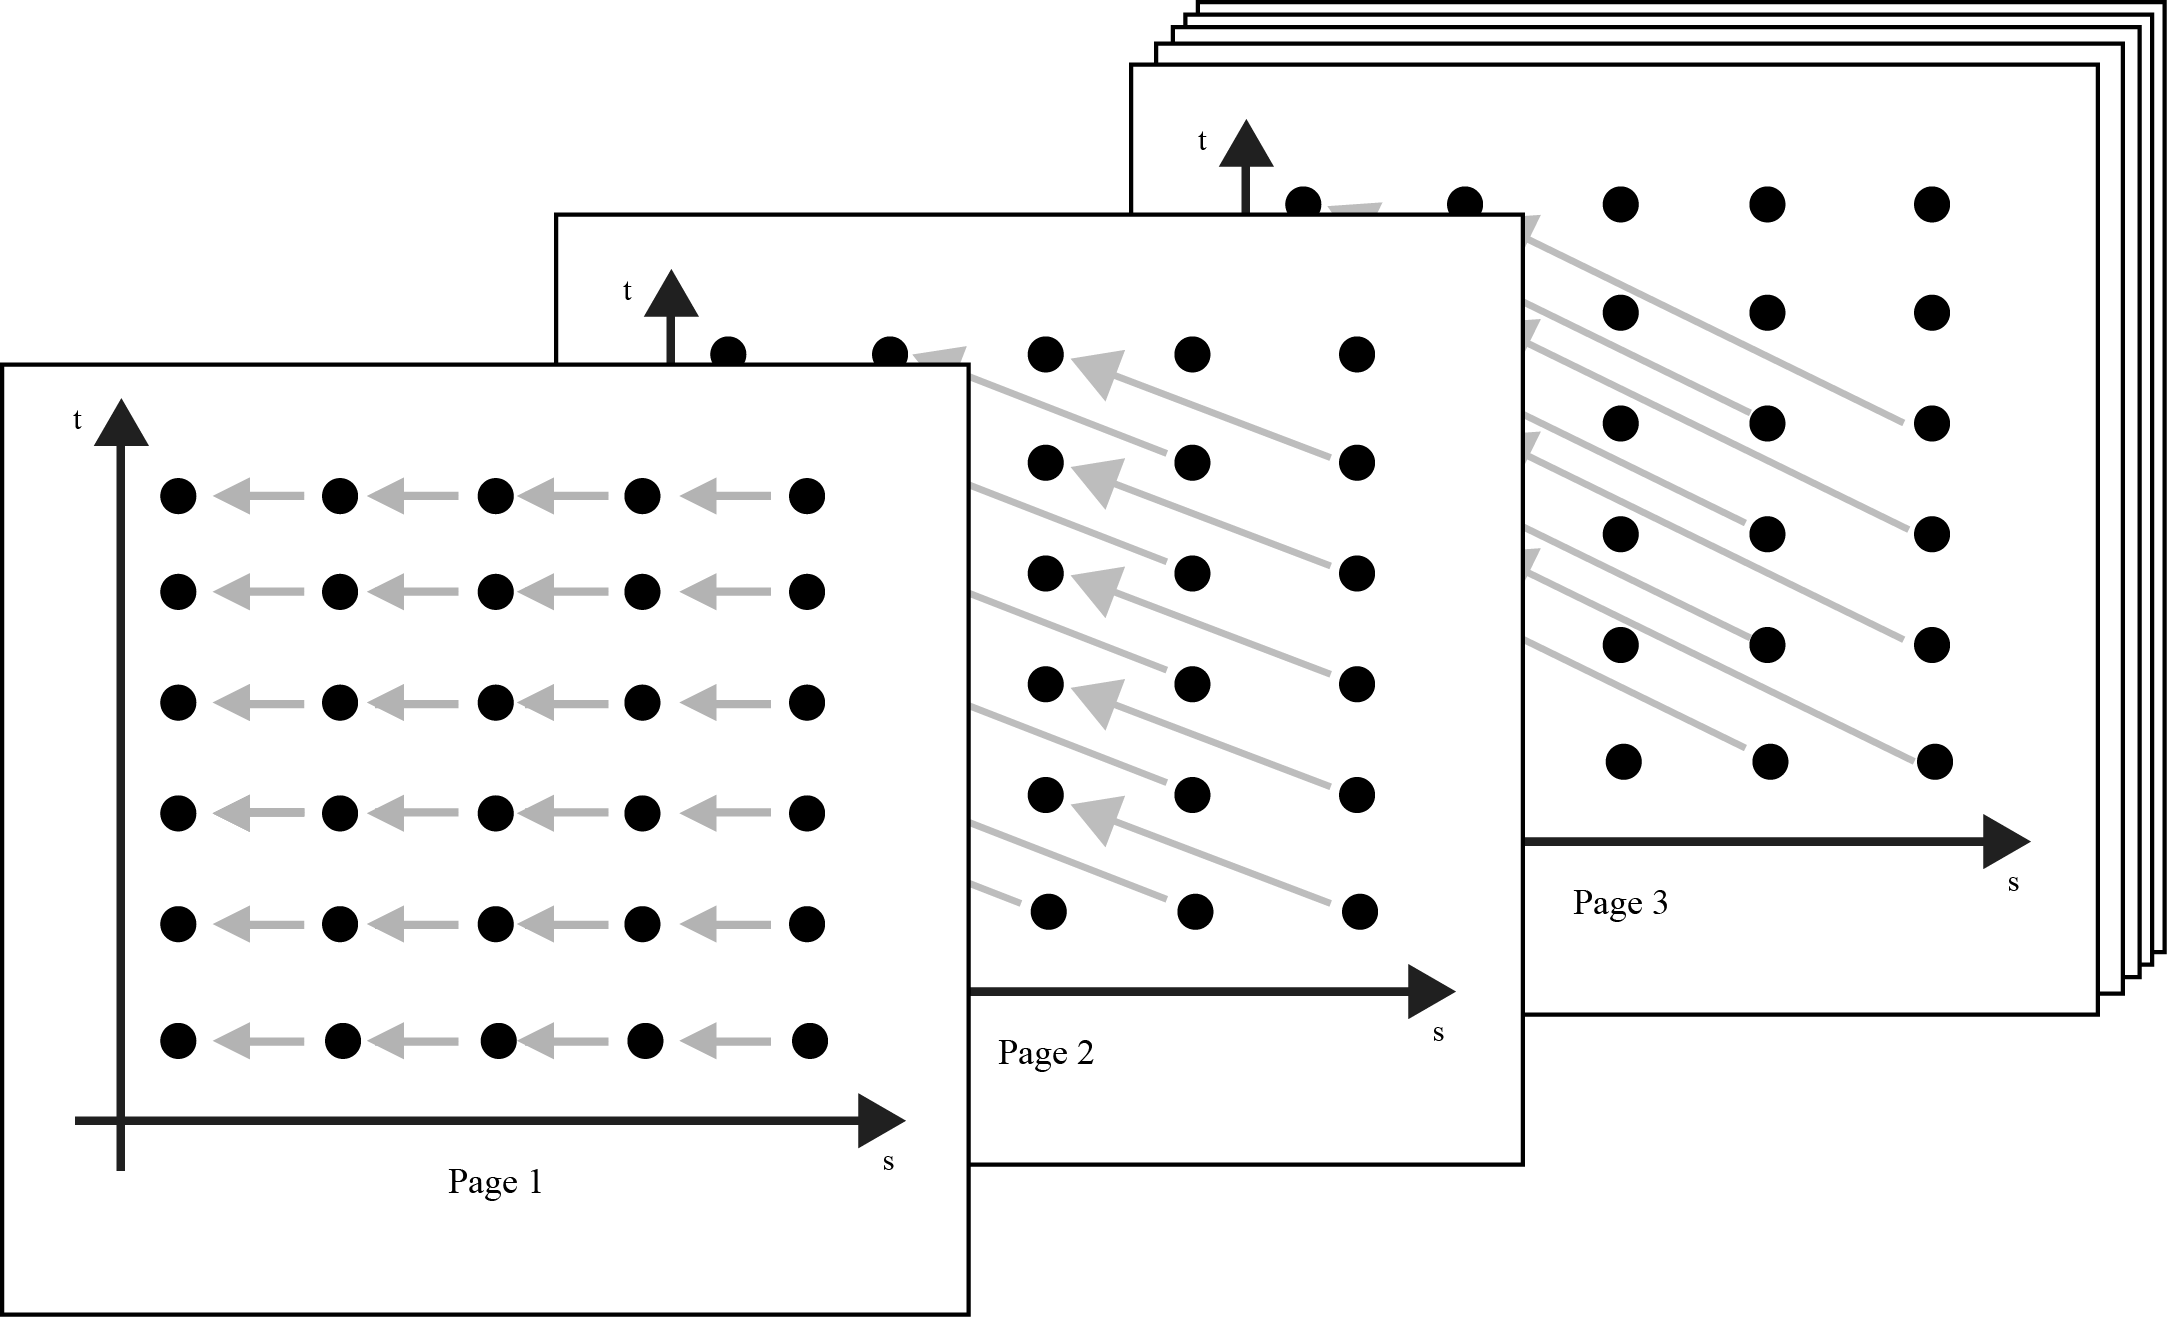
\includegraphics[width=\linewidth,height=0.45\textheight,keepaspectratio]{figures/cover.png}
  \end{center}
       \begin{minipage}{.35\linewidth}
    \begin{flushleft}
      \vspace{2em}
      {\fontsize{6pt}{2pt} \textit{Notes: These are notes live-tex'd
from a graduate course in 4-Manifolds taught by Philip Engel at the
University of Georgia in Spring 2021. As such, any errors or
inaccuracies are almost certainly my own. } } \\
    \end{flushleft}
    \end{minipage}
    \hfill
    \begin{minipage}{.65\linewidth}
    \end{minipage}
  }







\begin{document}

\date{}
\author{D. Zack Garza}
\maketitle
\begin{flushleft}
\textit{D. Zack Garza} \\
\textit{University of Georgia} \\
  \textit{\href{mailto: dzackgarza@gmail.com}{dzackgarza@gmail.com}} \\
{\tiny \textit{Last updated:} 2021-03-08 }
\end{flushleft}


\newpage

% Note: addsec only in KomaScript
\addsec{Table of Contents}
\tableofcontents
\newpage

\hypertarget{tuesday-january-12}{%
\section{Tuesday, January 12}\label{tuesday-january-12}}

\hypertarget{background}{%
\subsection{Background}\label{background}}

From Phil's email:

There are very few references in the notes, and I'll try to update them
to include more as we go. Personally, I found the following online
references particularly useful:

\begin{itemize}
\item
  Dietmar Salamon: Spin Geometry and Seiberg-Witten Invariants
  \autocite{Dietmar99}
\item
  Richard Mandelbaum: Four-dimensional Topology: An Introduction
  \autocite{Mandelbaum1980}

  \begin{itemize}
  \tightlist
  \item
    This book has a nice introduction to surgery aspects of
    four-manifolds, but as a warning: It was published right before
    Freedman's famous theorem. For instance, the existence of an exotic
    R\^{}4 was not known. This actually makes it quite useful, as a
    summary of what was known before, and provides the historical
    context in which Freedman's theorem was proven.
  \end{itemize}
\item
  Danny Calegari: Notes on 4-Manifolds \autocite{Calegari}
\item
  Yuli Rudyak: Piecewise Linear Structures on Topological Manifolds
  \autocite{Rudyak}
\item
  Akhil Mathew: The Dirac Operator \autocite{Matthew}
\item
  Tom Weston: An Introduction to Cobordism Theory \autocite{Weston}

  A wide variety of lecture notes on the Atiyah-Singer index theorem,
  which are available online.
\end{itemize}

\hypertarget{introduction}{%
\subsection{Introduction}\label{introduction}}

\begin{definition}[Topological Manifold]

Recall that a \textbf{topological manifold} (or \(C^0\) manifold) \(X\)
is a Hausdorff topological space \emph{locally homeomorphic} to
\({\mathbb{R}}^n\) with a countable topological base, so we have charts
\(\phi_u: U\to {\mathbb{R}}^n\) which are homeomorphisms from open sets
covering \(X\).

\end{definition}

\begin{example}[The circle]

\(S^1\) is covered by two charts homeomorphic to intervals:

\begin{figure}
\centering
\resizebox{\columnwidth}{!}{%
\begin{tikzpicture}
\node (node_one) at (0,0) { \fontsize{45pt}{1em} \import{/home/zack/SparkleShare/github.com/Notes/Class_Notes/2021/Spring/FourManifolds/sections/figures/}{2021-01-16_21-54.pdf_tex} };
\end{tikzpicture}
}
\end{figure}

\end{example}

\begin{remark}

Maps that are merely continuous are poorly behaved, so we may want to
impose extra structure. This can be done by imposing restrictions on the
transition functions, defined as
\begin{align*}
t_{uv} \coloneqq\varphi_V \to \varphi_U ^{-1} : \varphi_U(U \cap V) \to \varphi_V(U \cap V)
.\end{align*}

\end{remark}

\begin{definition}[Restricted Structures on Manifolds]

\envlist

\begin{itemize}
\item
  We say \(X\) is a \textbf{PL manifold} if and only if \(t_{UV}\) are
  piecewise-linear. Note that an invertible PL map has a PL inverse.
\item
  We say \(X\) is a \textbf{\(C^k\) manifold} if they are \(k\) times
  continuously differentiable, and \textbf{smooth} if infinitely
  differentiable.
\item
  We say \(X\) is \textbf{real-analytic} if they are locally given by
  convergent power series.
\item
  We say \(X\) is \textbf{complex-analytic} if under the identification
  \({\mathbb{R}}^n \cong {\mathbb{C}}^{n/2}\) if they are holomorphic,
  i.e.~the differential of \(t_{UV}\) is complex linear.
\item
  We say \(X\) is a \textbf{projective variety} if it is the vanishing
  locus of homogeneous polynomials on \({\mathbb{CP}}^N\).
\end{itemize}

\end{definition}

\begin{remark}

Is this a strictly increasing hierarchy? It's not clear e.g.~that every
\(C^k\) manifold is PL.

\end{remark}

\begin{question}

Consider \({\mathbb{R}}^n\) as a topological manifold: are any two
smooth structures on \({\mathbb{R}}^n\) diffeomorphic?

\end{question}

\begin{remark}

Fix a copy of \({\mathbb{R}}\) and form a single chart
\({\mathbb{R}}\xrightarrow{\operatorname{id}} {\mathbb{R}}\). There is
only a single transition function, the identity, which is smooth. But
consider
\begin{align*}
X &\to {\mathbb{R}}\\
t &\mapsto t^3
.\end{align*}
This is also a smooth structure on \(X\), since the transition function
is the identity. This yields a different smooth structure, since these
two charts don't like in the same maximal atlas. Otherwise there would
be a transition function of the form \(t_{VU}: t\mapsto t^{1/3}\), which
is not smooth at zero. However, the map
\begin{align*}
X &\to X \\
t &\mapsto t^3
.\end{align*}
defines a diffeomorphism between the two smooth structures.

\end{remark}

\begin{claim}

\({\mathbb{R}}\) admits a unique smooth structure.

\end{claim}

\begin{proof}[sketch]

Let \(\tilde {\mathbb{R}}\) be some exotic \({\mathbb{R}}\), i.e.~a
smooth manifold homeomorphic to \({\mathbb{R}}\). Cover this by
coordinate charts to the standard \({\mathbb{R}}\):

\begin{figure}
\centering
\resizebox{\columnwidth}{!}{%
\begin{tikzpicture}
\node (node_one) at (0,0) { \import{/home/zack/SparkleShare/github.com/Notes/Class_Notes/2021/Spring/FourManifolds/sections/figures}{2021-01-16_22-31.pdf_tex} };
\end{tikzpicture}
}
\end{figure}

\begin{fact}

There exists a cover which is \emph{locally finite} and supports a
\emph{partition of unity}: a collection of smooth functions
\(f_i: U_i \to {\mathbb{R}}\) with \(f_i \geq 0\) and
\({\operatorname{supp}}f \subseteq U_i\) such that \(\sum f_i = 1\)
(\emph{i.e., bump functions}). It is also a purely topological fact that
\(\tilde {\mathbb{R}}\) is orientable.

\end{fact}

So we have bump functions:

\begin{figure}
\centering
\resizebox{\columnwidth}{!}{%
\begin{tikzpicture}
\node (node_one) at (0,0) { \import{/home/zack/SparkleShare/github.com/Notes/Class_Notes/2021/Spring/FourManifolds/sections/figures}{2021-01-16_22-37.pdf_tex} };
\end{tikzpicture}
}
\end{figure}

Take a smooth vector field \(V_i\) on \(U_i\) everywhere aligning with
the orientation. Then \(\sum f_i V_i\) is a smooth nowhere vector field
on \(X\) that is nowhere zero in the direction of the orientation.
Taking the associated flow
\begin{align*}
{\mathbb{R}}&\to \tilde {\mathbb{R}}\\
t &\mapsto \varphi(t)
.\end{align*}
such that \(\varphi'(t) = V(\varphi(t))\). Then \(\varphi\) is a smooth
map that defines a diffeomorphism. This follows from the fact that the
vector field is everywhere positive.

\begin{slogan}

To understand smooth structures on \(X\), we should try to solve
differential equations on \(X\).

\end{slogan}

\end{proof}

\begin{remark}

Note that here we used the existence of a global frame, i.e.~a
trivialization of the tangent bundle, so this doesn't quite work for
e.g.~\(S^2\).

\end{remark}

\begin{question}

What is the difference between all of the above structures? Are there
obstructions to admitting any particular one?

\end{question}

\begin{answer}

\envlist

\begin{enumerate}
\def\labelenumi{\arabic{enumi}.}
\item
  (Munkres) Every \(C^1\) structure gives a unique \(C^k\) and
  \(C^ \infty\) structure.\footnote{Note that this doesn't start at
    \(C^0\), so topological manifolds are genuinely different! There
    exist topological manifolds with no smooth structure.}
\item
  (Grauert) Every \(C^ \infty\) structure gives a unique real-analytic
  structure.
\item
  Every PL manifold admits a smooth structure in \(\dim X \leq 7\), and
  it's unique in \(\dim X\leq 6\), and above these dimensions there
  exists PL manifolds with no smooth structure.
\item
  (Kirby--Siebenmann) Let \(X\) be a topological manifold of
  \(\dim X\geq 5\), then there exists a cohomology class
  \(\operatorname{ks}(X) \in H^4(X; {\mathbb{Z}}/2{\mathbb{Z}})\) which
  is 0 if and only if \(X\) admits a PL structure. Moreover, if
  \(\operatorname{ks}(X) = 0\), then (up to concordance) the set of PL
  structures is given by \(H^3(X; {\mathbb{Z}}/2{\mathbb{Z}})\).
\item
  (Moise) Every topological manifold in \(\dim X\leq 3\) admits a unique
  smooth structure.
\item
  (Smale et al.): In \(\dim X\geq 5\), the number of smooth structures
  on a topological manifold \(X\) is finite. In particular,
  \({\mathbb{R}}^n\) for \(n \neq 4\) has a unique smooth structure. So
  dimension 4 is interesting!
\item
  (Taubes) \({\mathbb{R}}^4\) admits uncountably many non-diffeomorphic
  smooth structures.
\item
  A compact oriented smooth surface \(\Sigma\), the space of
  complex-analytic structures is a complex orbifold \footnote{Locally
    admits a chart to \({\mathbb{C}}^n/ \Gamma\) for \(\Gamma\) a finite
    group.} of dimension \(3g-2\) where \(g\) is the genus of
  \(\Sigma\), up to biholomorphism (i.e.~\emph{moduli}).
\end{enumerate}

\end{answer}

\begin{remark}

Kervaire-Milnor: \(S^7\) admits 28 smooth structures, which form a
group.

\end{remark}

\hypertarget{friday-january-15}{%
\section{Friday, January 15}\label{friday-january-15}}

\begin{remark}

Let
\begin{align*}
V &\coloneqq\left\{{a^2 + b^2 + c^2 + d^3 + e^{6k-1} = 0}\right\} \subseteq {\mathbb{C}}^5 \\
S_\varepsilon&\coloneqq\left\{{ {\left\lvert {a} \right\rvert}^2 + {\left\lvert {b} \right\rvert}^2 + {\left\lvert {c} \right\rvert}^2 + {\left\lvert {d} \right\rvert}^2 + {\left\lvert {e} \right\rvert}^2}\right\}
.\end{align*}
Then \(V_k \cap S_\varepsilon\cong S^7\) is a homeomorphism, and taking
\(k=1,2,\cdots, 28\) yields the 28 smooth structures on \(S^7\). Note
that \(V_k\) is the cone over \(V_k \cap S_\varepsilon\).

\begin{figure}
\centering
\resizebox{\columnwidth}{!}{%
\begin{tikzpicture}
\node (node_one) at (0,0) { 
\fontsize{25pt}{1em} 
\import{/home/zack/SparkleShare/github.com/Notes/Class_Notes/2021/Spring/FourManifolds/sections/figures/}{2021-01-15_13-54.pdf_tex} };
\end{tikzpicture}
}
\end{figure}

\begin{quote}
? Admits a smooth structure, and
\(\mkern 1.5mu\overline{\mkern-1.5muV\mkern-1.5mu}\mkern 1.5mu_k \subseteq {\mathbb{CP}}^5\)
admits no smooth structure.
\end{quote}

\end{remark}

\begin{question}

Is every triangulable manifold PL, i.e.~homeomorphic to a simplicial
complex?

\end{question}

\begin{answer}

No! Given a simplicial complex, there is a notion of the
\textbf{combinatorial link} \(L_V\) of a vertex \(V\):

\begin{figure}
\centering
\resizebox{\columnwidth}{!}{%
\begin{tikzpicture}
\node (node_one) at (0,0) {
\import{/home/zack/SparkleShare/github.com/Notes/Class_Notes/2021/Spring/FourManifolds/sections/figures/}{2021-01-15_13-57.pdf_tex} };
\end{tikzpicture}
}
\end{figure}

It turns out that there exist simplicial manifolds such that the link is
not homeomorphic to a sphere, whereas every PL manifold admits a ``PL
triangulation'' where the links are spheres.

\end{answer}

\begin{remark}

What's special in dimension 4? Recall the \textbf{Kirby-Siebenmann}
invariant \(\operatorname{ks}(x) \in H^4(X; {\mathbb{Z}}_2)\) for \(X\)
a topological manifold where \(\operatorname{ks}(X) = 0 \iff X\) admits
a PL structure, with the caveat that \(\dim X \geq 5\). We can use this
to cook up an invariant of 4-manifolds.

\end{remark}

\begin{definition}[Kirby-Siebenmann Invariant of a 4-manifold]

Let \(X\) be a topological 4-manifold, then
\begin{align*}
\operatorname{ks}(X) \coloneqq\operatorname{ks}(X \times{\mathbb{R}})
.\end{align*}

\end{definition}

\begin{remark}

Recall that in \(\dim X\geq 7\), every PL manifold admits a smooth
structure, and we can note that
\begin{align*}
H^4(X; {\mathbb{Z}}_2) = H^4(X \times{\mathbb{R}}; {\mathbb{Z}}_2) = {\mathbb{Z}}_2,
.\end{align*}
since every oriented 4-manifold admits a fundamental class. Thus
\begin{align*}
\operatorname{ks}(X) = 
\begin{cases}
0 & X \times{\mathbb{R}}\text{ admits a PL and smooth structure} 
\\
1 & X \times{\mathbb{R}}\text{ admits no PL or smooth structures }.
\end{cases}
\end{align*}

\end{remark}

\begin{remark}

\(\operatorname{ks}(X) \neq 0\) implies that \(X\) has no smooth
structure, since \(X \times{\mathbb{R}}\) doesn't. Note that it was not
known if this invariant was nonzero for a while!

\end{remark}

\begin{remark}

Note that \(H^2(X; {\mathbb{Z}})\) admits a symmetric bilinear form
\(Q_X\) defined by
\begin{align*}
{\left\langle { \alpha},~{ \beta} \right\rangle} \mapsto \int_X \alpha\wedge \beta = \alpha \smile\beta([X]) \in {\mathbb{Z}}
.\end{align*}
where \([X]\) is the fundamental class.

\end{remark}

\hypertarget{main-theorems-for-the-course}{%
\section{Main Theorems for the
Course}\label{main-theorems-for-the-course}}

Proving the following theorems is the main goal of this course.

\begin{theorem}[Freedman]

If \(X, Y\) are compact oriented topological 4-manifolds, then
\(X\cong Y\) are homeomorphic if and only if
\(\operatorname{ks}(X) = \operatorname{ks}(Y)\) and \(Q_X \cong Q_Y\)
are isometric, i.e.~there exists an isometry
\begin{align*}
\varphi: H^2(X; {\mathbb{Z}}) \to H^2(Y; {\mathbb{Z}})
.\end{align*}
that preserves the two bilinear forms in the sense that
\({\left\langle {\varphi \alpha},~{ \varphi \beta} \right\rangle} = {\left\langle { \alpha},~{ \beta} \right\rangle}\).

Conversely, every \textbf{unimodular} bilinear form appears as
\(H^2(X; {\mathbb{Z}})\) for some \(X\), i.e.~the pairing induces a map
\begin{align*}
H^2(X; {\mathbb{Z}}) &\to H^2(X; {\mathbb{Z}})^\vee\\
\alpha \mapsto {\left\langle { \alpha },~{ {\,\cdot\,}} \right\rangle}
.\end{align*}
which is an isomorphism. This is essentially a classification of
simply-connected 4-manifolds.

\end{theorem}

\begin{remark}

Note that preservation of a bilinear form is a stand-in for ``being an
element of the orthogonal group'', where we only have a lattice instead
of a full vector space.

\end{remark}

\begin{remark}

There is a map
\(H^2(X; {\mathbb{Z}}) \xrightarrow{PD} H_2(X; {\mathbb{Z}})\) from
Poincaré , where we can think of elements in the latter as closed
surfaces \([\Sigma]\), and
\begin{align*}
{\left\langle { \Sigma_1 },~{ \Sigma_2 } \right\rangle} = \text{signed number of intersections points of } \Sigma_1 \pitchfork\Sigma_2
.\end{align*}
Note that Freedman's theorem is only about homeomorphism, and is not
true smoothly. This gives a way to show that two 4-manifolds are
homeomorphic, but this is hard to prove! So we'll black-box this, and
focus on ways to show that two \emph{smooth} 4-manifolds are \emph{not}
diffeomorphic, since we want homeomorphic but non-diffeomorphic
manifolds.

\end{remark}

\begin{definition}[Signature]

The \textbf{signature} of a topological 4- manifold is the signature of
\(Q_X\), where we note that \(Q_X\) is a symmetric nondegenerate
bilinear form on \(H^2(X; {\mathbb{R}})\) and for some \(a, b\)
\begin{align*}
(H^2(X; {\mathbb{R}}), Q_x) \xrightarrow{\text{isometric}} {\mathbb{R}}^{a, b}
.\end{align*}
where \(a\) is the number of \(+1\)s appearing in the matrix and \(b\)
is the number of \(-1\)s. This is \({\mathbb{R}}^{ab}\) where
\(e_i^2 = 1, i=1\cdots a\) and \(e_i^2 = -1, i=a+1, \cdots b\), and is
thus equipped with a specific bilinear form corresponding to the Gram
matrix of this basis.
\begin{align*}
\begin{bmatrix}
1 & 0 & 0 & 0 & 0
\\
0 & 1 & 0 & 0 & 0
\\
0 & 0 & \ddots & 0 & 0
\\
0 & 0 & 0 & -1 & 0
\\
0 & 0 & 0 & 0 & -1
\end{bmatrix}
= I_{a\times a} \oplus -I_{b \times b}
.\end{align*}
Then the signature is \(a-b\), the dimension of the positive-definite
space minus the dimension of the negative-definite space.

\end{definition}

\begin{theorem}[Rokhlin's Theorem]

Suppose
\({\left\langle { \alpha},~{\alpha} \right\rangle} \in 2{\mathbb{Z}}\)
and \(\alpha\in H^2(X; {\mathbb{Z}})\) and \(X\) a simply connected
\textbf{smooth} 4-manifold. Then 16 divides \(\operatorname{sig}(X)\).

\end{theorem}

\begin{remark}

Note that Freedman's theorem implies that there exists topological
4-manifolds with no smooth structure.

\end{remark}

\begin{theorem}[Donaldson]

Let \(X\) be a smooth simply-connected 4-manifold. If \(a=0\) or
\(b=0\), then \(Q_X\) is diagonalizable and there exists an orthonormal
basis of \(H^2(X; {\mathbb{Z}})\).

\end{theorem}

\begin{remark}

This comes from Gram-Schmidt, and restricts what types of intersection
forms can occur.

\end{remark}

\hypertarget{warm-up-mathbbr2-has-a-unique-smooth-structure}{%
\subsection{\texorpdfstring{Warm Up: \({\mathbb{R}}^2\) Has a Unique
Smooth
Structure}{Warm Up: \{\textbackslash mathbb\{R\}\}\^{}2 Has a Unique Smooth Structure}}\label{warm-up-mathbbr2-has-a-unique-smooth-structure}}

\begin{remark}

Last time we showed \({\mathbb{R}}^1\) had a unique smooth structure, so
now we'll do this for \({\mathbb{R}}^2\). The strategy of solving a
differential equation, we'll now sketch the proof.

\end{remark}

\begin{definition}[Riemannian Metrics]

A \textbf{Riemannian metric} \(g\in \operatorname{Sym}^2 T^*X\) for
\(X\) a smooth manifold is a metric on every \(T_p X\) given by
\begin{align*}
g_p: T_pX \times T_p X &\to {\mathbb{R}}\\
g(v, v) \geq 0, g(v,v) = 0 \iff v=0
.\end{align*}

\end{definition}

\begin{definition}[Almost complex structure]

An \textbf{almost complex structure} is a
\(J\in \mathop{\mathrm{End}}(TX)\) such that
\(J^2 = -\operatorname{id}\).

\end{definition}

\begin{remark}

Let \(e\in T_p X\) and \(e\neq 0\), then if \(X\) is a surface then
\(\left\{{e, Je}\right\}\) is a basis of \(T_p X\).

\begin{figure}
\centering
\resizebox{\columnwidth}{!}{%
\begin{tikzpicture}
\node (node_one) at (0,0) { 
\fontsize{25pt}{1em} 
\import{/home/zack/SparkleShare/github.com/Notes/Class_Notes/2021/Spring/FourManifolds/sections/figures/}{2021-01-15_14-33.pdf_tex} };
\end{tikzpicture}
}
\end{figure}

This is a basis because if \(Je\) and \(e\) are parallel, then ??? In
particular, \(J_p\) is determined by a point in
\({\mathbb{R}}^2\setminus\left\{{\text{the }x{\hbox{-}}\text{axis}}\right\}\)

\end{remark}

\hypertarget{sketch-of-proof}{%
\subsubsection{Sketch of Proof}\label{sketch-of-proof}}

Let \(\tilde {\mathbb{R}}^2\) be an exotic \({\mathbb{R}}^2\).

\hypertarget{step-1}{%
\paragraph{Step 1}\label{step-1}}

Choose a metric on \(\tilde {\mathbb{R}}^2\) \(g \coloneqq\sum f_I g_i\)
with \(g_i\) metrics on coordinate charts \(U_i\) and \(f_i\) a
partition of unity.

\hypertarget{step-2}{%
\paragraph{Step 2}\label{step-2}}

Find an almost complex structure on \(\tilde {\mathbb{R}}^2\). Choosing
an orientation of \(\tilde {\mathbb{R}}^2\), \(g\) defines a unique
almost complex structure
\(J_p e \coloneqq f\in T_p \tilde {\mathbb{R}}^2\) such that

\begin{itemize}
\tightlist
\item
  \(g(e, e) = g(f, f)\)
\item
  \(g(e, f) = 0\).
\item
  \(\left\{{e, f}\right\}\) is an oriented basis of
  \(T_p \tilde {\mathbb{R}}^2\)
\end{itemize}

This is because after choosing \(e\), there are two orthogonal vectors,
but only one choice yields an \emph{oriented} basis.

\begin{figure}
\centering
\resizebox{\columnwidth}{!}{%
\begin{tikzpicture}
\node (node_one) at (0,0) {
\fontsize{25pt}{1em} 
  \import{/home/zack/SparkleShare/github.com/Notes/Class_Notes/2021/Spring/FourManifolds/sections/figures/}{2021-01-15_14-39.pdf_tex}
  };
\end{tikzpicture}
}
\end{figure}

\hypertarget{step-3}{%
\paragraph{Step 3}\label{step-3}}

We then apply a theorem:

\begin{theorem}[?]

Any almost complex structure on a surface comes from a complex
structure, in the sense that there exist charts
\(\varphi_i: U_i \to {\mathbb{C}}\) such that \(J\) is multiplication by
\(i\).

\end{theorem}

So \(d \varphi(J \cdot e) = i \cdot d \varphi_i (e)\), and
\((\tilde {\mathbb{R}}^2, J)\) is a complex manifold. Since it's simply
connected, the Riemann Mapping Theorem shows that it's biholomorphic to
\({\mathbb{D}}\) or \({\mathbb{C}}\), both of which are diffeomorphic to
\({\mathbb{R}}^2\).

\begin{quote}
See the Newlander-Nirenberg theorem, a result in complex geometry.
\end{quote}

\hypertarget{lecture-3-wednesday-january-20}{%
\section{Lecture 3 (Wednesday, January
20)}\label{lecture-3-wednesday-january-20}}

Today: some background material on sheaves, bundles, connections.

\hypertarget{sheaves}{%
\subsection{Sheaves}\label{sheaves}}

\begin{definition}[Presheaves and Sheaves]

Recall that if \(X\) is a topological space, a \textbf{presheaf} of
abelian groups \(\mathcal{F}\) is an assignment \(U\to \mathcal{F}(U)\)
of an abelian group to every open set \(U \subseteq X\) together with a
restriction map \(\rho_{UV}: \mathcal{F}(U) \to \mathcal{F}(V)\) for any
inclusion \(V \subseteq U\) of open sets. This data has to satisfying
certain conditions:

\begin{enumerate}
\def\labelenumi{\alph{enumi}.}
\item
  \(\mathcal{F}(\emptyset) = 0\), the trivial abelian group.
\item
  \(\rho_{UU}: \mathcal{F}(U) \to \mathcal{F}(U) = \operatorname{id}_{\mathcal{F}(U) }\)
\item
  Compatibility if restriction is taken in steps:
  \(U \subseteq V \subseteq W \implies \rho_{VW} \circ \rho_{UV} = \rho_{UW}\).
\end{enumerate}

We say \(\mathcal{F}\) is a \textbf{sheaf} if additionally:

\begin{enumerate}
\def\labelenumi{\alph{enumi}.}
\setcounter{enumi}{3}
\tightlist
\item
  Given \(s_i \in \mathcal{F}(U_i)\) such that
  \(\rho_{U_i \cap U_j} (s_i) = \rho_{U_i \cap U_j} (s_j)\) implies that
  there exists a unique \(s\in \mathcal{F}(\bigcup_i U_i)\) such that
  \(\rho_{U_i}(s) = s_i\).
\end{enumerate}

\begin{figure}
\centering
\resizebox{\columnwidth}{!}{%
\begin{tikzpicture}
\node (node_one) at (0,0) { 
\fontsize{45pt}{1em} 
\import{/home/zack/SparkleShare/github.com/Notes/Class_Notes/2021/Spring/FourManifolds/sections/figures}{2021-01-20_13-59.pdf_tex} };
\end{tikzpicture}
}
\end{figure}

\end{definition}

\begin{example}[?]

Let \(X\) be a topological manifold, then
\(\mathcal{F}\coloneqq C^0({\,\cdot\,}, {\mathbb{R}})\) the set of
continuous functionals form a sheaf. We have a diagram

\begin{center}
\begin{tikzcd}
    U && {C^0(U; {\mathbb{R}})} \\
    \\
    V && {C^0(V; {\mathbb{R}})}
    \arrow[hook, from=3-1, to=1-1]
    \arrow["{\text{restrict cts. functions}}", dashed, hook, from=1-3, to=3-3]
    \arrow["{\mathcal{F}}", from=1-1, to=1-3]
    \arrow["{\mathcal{F}}"', from=3-1, to=3-3]
\end{tikzcd}
\end{center}

\begin{quote}
\href{https://q.uiver.app/?q=WzAsNCxbMCwwLCJVIl0sWzAsMiwiViJdLFsyLDAsIkNeMChVOyBcXFJSKSJdLFsyLDIsIkNeMChWOyBcXFJSKSJdLFsxLDAsIiIsMCx7InN0eWxlIjp7InRhaWwiOnsibmFtZSI6Imhvb2siLCJzaWRlIjoidG9wIn19fV0sWzIsMywiXFx0ZXh0e3Jlc3RyaWN0IGN0cy4gZnVuY3Rpb25zfSIsMCx7InN0eWxlIjp7InRhaWwiOnsibmFtZSI6Imhvb2siLCJzaWRlIjoidG9wIn0sImJvZHkiOnsibmFtZSI6ImRhc2hlZCJ9fX1dLFswLDIsIlxcbWF0aGNhbHtGfSJdLFsxLDMsIlxcbWF0aGNhbHtGfSIsMl1d}{Link
to diagram}
\end{quote}

Property (d) holds because given sections
\(s_i \in C^0(U_i; {\mathbb{R}})\) agreeing on overlaps, so
\({ \left.{{s_i}} \right|_{{U_i \cap U_j}} } = { \left.{{s_j}} \right|_{{U_i \cap U_j}} }\),
there exists a unique \(s\in C^0(\bigcup_i U_i; {\mathbb{R}})\) such
that \({ \left.{{s}} \right|_{{U_i}} } = s_i\) for all \(i\) --
continuous functions glue.

\end{example}

\begin{remark}

Recall that we discussed various structures on manifolds: PL,
continuous, smooth, complex-analytic, etc. We can characterize these by
their sheaves of functions, which we'll denote \({\mathcal{O}}\). For
example, \({\mathcal{O}}\coloneqq C^0({\,\cdot\,}; {\mathbb{R}})\) for
topological manifolds, and
\({\mathcal{O}}\coloneqq C^ \infty ({\,\cdot\,}; {\mathbb{R}})\) is the
sheaf for smooth manifolds. Note that this also works for PL functions,
since pullbacks of PL functions are again PL. For complex manifolds, we
set \({\mathcal{O}}\) to be the sheaf of holomorphic functions.

\end{remark}

\begin{example}[Locally Constant Sheaves]

Let \(A\in {\mathsf{Ab}}\) be an abelian group, then \(\underline{A}\)
is the sheaf defined by setting \(\underline{A}(U)\) to be the locally
constant functions \(U\to A\). E.g. let
\(X \in {\mathsf{Mfd}}_{{\mathsf{Top}}}\) be a topological manifold,
then \(\underline{{\mathbb{R}}}(U) = {\mathbb{R}}\) if \(U\) is
connected since locally constant \(\implies\) globally constant in this
case.

\end{example}

\begin{warnings}

Note that the presheaf of constant functions doesn't satisfy (d)! Take
\({\mathbb{R}}\) and a function with two different values on disjoint
intervals:

\begin{figure}
\centering
\resizebox{\columnwidth}{!}{%
\begin{tikzpicture}
\node (node_one) at (0,0) { 
\fontsize{41pt}{1em} 
\import{/home/zack/SparkleShare/github.com/Notes/Class_Notes/2021/Spring/FourManifolds/sections/figures}{2021-01-20_14-11.pdf_tex} };
\end{tikzpicture}
}
\end{figure}

Note that
\({ \left.{{s_1}} \right|_{{U_1 \cap U_2}} } = { \left.{{s_2}} \right|_{{U_1 \cap U_2}} }\)
since the intersection is empty, but there is no constant function that
restricts to the two different values.

\end{warnings}

\hypertarget{bundles}{%
\subsection{Bundles}\label{bundles}}

\begin{remark}

Let \(\pi: \mathcal{E}\to X\) be a \textbf{vector bundle}, so we have
local trivializations \(\pi ^{-1} (U) \xrightarrow{h_u} Y^d \times U\)
where we take either \(Y={\mathbb{R}}, {\mathbb{C}}\), such that
\(h_v \circ h_u ^{-1}\) preserves the fibers of \(\pi\) and acts
linearly on each fiber of \(Y\times(U \cap V)\). Define
\begin{align*}
t_{UV}: U \cap V \to \operatorname{GL}_d(Y)
\end{align*}
where we require that \(t_{UV}\) is continuous, smooth,
complex-analytic, etc depending on the context.

\begin{figure}
\centering
\resizebox{\columnwidth}{!}{%
\begin{tikzpicture}
\node (node_one) at (0,0) { 
\fontsize{47pt}{1em} 
\import{/home/zack/SparkleShare/github.com/Notes/Class_Notes/2021/Spring/FourManifolds/sections/figures}{2021-01-20_14-17.pdf_tex} };
\end{tikzpicture}
}
\end{figure}

\end{remark}

\begin{example}[Bundles over $S^1$]

There are two \({\mathbb{R}}^1\) bundles over \(S^1\):

\begin{figure}
\centering
\resizebox{\columnwidth}{!}{%
\begin{tikzpicture}
\node (node_one) at (0,0) { 
\fontsize{32pt}{1em} 
\import{/home/zack/SparkleShare/github.com/Notes/Class_Notes/2021/Spring/FourManifolds/sections/figures}{2021-01-20_14-20.pdf_tex} };
\end{tikzpicture}
}
\end{figure}

Note that the Mobius bundle is not trivial, but can be locally
trivialized.

\end{example}

\begin{remark}

We abuse notation: \(\mathcal{E}\) is also a sheaf, and we write
\(\mathcal{E}(U)\) to be the set of sections \(s: U\to \mathcal{E}\)
where \(s\) is continuous, smooth, holomorphic, etc where
\(\pi \circ s = \operatorname{id}_U\). I.e. a bundle is a sheaf in the
sense that its sections \emph{form} a sheaf.

\end{remark}

\begin{example}[?]

The trivial line bundle gives the sheaf \({\mathcal{O}}\) : maps
\(U \xrightarrow{s} U\times Y\) for \(Y={\mathbb{R}}, {\mathbb{C}}\)
such that \(\pi \circ s = \operatorname{id}\) are the same as maps
\(U\to Y\).

\end{example}

\begin{definition}[$\OO\dash$modules]

An \textbf{\({\mathcal{O}}{\hbox{-}}\)module} is a sheaf \(\mathcal{F}\)
such that \(\mathcal{F}(U)\) has an action of \(\mathcal{O}(U)\)
compatible with restriction.

\end{definition}

\begin{example}[?]

If \(\mathcal{E}\) is a vector bundle, then \(\mathcal{E}(U)\) has a
natural action of \({\mathcal{O}}(U)\) given by
\(f\curvearrowright s \coloneqq fs\), i.e.~just multiplying functions.

\end{example}

\begin{example}[Non-example]

The locally constant sheaf \(\underline{{\mathbb{R}}}\) is not an
\({\mathcal{O}}{\hbox{-}}\)module: there isn't natural action since the
sections of \({\mathcal{O}}\) are generally non-constant functions, and
multiplying a constant function by a non-constant function doesn't
generally give back a constant function.

\end{example}

We'd like a notion of maps between sheaves:

\begin{definition}[Morphisms of Sheaves]

A \textbf{morphism} of sheaves \(\mathcal{F} \to \mathcal{G}\) is a
group morphism \(\varphi(U): \mathcal{F}(U) \to \mathcal{G}(U)\) for all
opens \(U \subseteq X\) such that the diagram involving restrictions
commutes:

\begin{center}
\begin{tikzcd}
\mathcal{F}(U) 
\ar[r, "\phi(U)"] 
\ar[d, "\rho_{UV}"]
&
\mathcal{G}(U) 
\ar[d, "\rho_{UV}"]
\\
\mathcal{F}(V) 
\ar[r, "\phi(V)"] 
&
\mathcal{F}(V) 
\end{tikzcd}
\end{center}

\end{definition}

\begin{example}[An $\OO\dash$module that is not a vector bundle.]

Let \(X = {\mathbb{R}}\) and define the \textbf{skyscraper sheaf} at
\(p \in {\mathbb{R}}\) as
\begin{align*}
{\mathbb{R}}_p(U) \coloneqq
\begin{cases}
{\mathbb{R}}& p\in U 
\\
0 & p\not\in U.
\end{cases}
.\end{align*}

The \({\mathcal{O}}(U){\hbox{-}}\)module structure is given by
\begin{align*}
{\mathcal{O}}(U) \times{\mathcal{O}}(U) &\to {\mathbb{R}}_p(U) \\
(f, s) &\mapsto f(p) s
.\end{align*}
This is not a vector bundle since \({\mathbb{R}}_p(U)\) is not an
infinite dimensional vector space, whereas the space of sections of a
vector bundle is generally infinite dimensional (?). Alternatively,
there are arbitrarily small punctured open neighborhoods of \(p\) for
which the sheaf makes trivial assignments.

\end{example}

\begin{example}[of morphisms]

Let \(X = {\mathbb{R}}\in {\mathsf{Mfd}}_{\operatorname{Sm}}\) viewed as
a smooth manifold, then multiplication by \(x\) induces a morphism of
structure sheaves:
\begin{align*}
(x \cdot): {\mathcal{O}}&\to {\mathcal{O}}\\
s & \mapsto x\cdot s
\end{align*}
for any \(x\in {\mathcal{O}}(U)\), noting that
\(x\cdot s\in {\mathcal{O}}(U)\) again.

\begin{exercise}[?]

Check that \(\ker \varphi\) is naturally a sheaf and
\(\ker(\varphi)(U) = \ker (\varphi(U)): \mathcal{F}(U) \to \mathcal{G}(U)\)

\end{exercise}

Here the kernel is trivial, i.e.~on any open \(U\) we have
\((x\cdot):{\mathcal{O}}(U) \hookrightarrow{\mathcal{O}}(U)\) is
injective. Taking the cokernel \(\operatorname{coker}(x\cdot)\) as a
presheaf, this assigns to \(U\) the quotient presheaf
\({\mathcal{O}}(U) / x{\mathcal{O}}(U)\), which turns out to be equal to
\({\mathbb{R}}_0\). So \({\mathcal{O}}\to {\mathbb{R}}_0\) by
restricting to the value at \(0\), and there is an exact sequence
\begin{align*}
0 \to {\mathcal{O}}\xrightarrow{(x\cdot)} {\mathcal{O}}\to {\mathbb{R}}_0 \to 0
.\end{align*}

This is one reason sheaves are better than vector bundles: the category
is closed under taking quotients, whereas quotients of vector bundles
may not be vector bundles.

\end{example}

\hypertarget{lecture-4-friday-january-22}{%
\section{Lecture 4 (Friday, January
22)}\label{lecture-4-friday-january-22}}

\hypertarget{the-exponential-exact-sequence}{%
\subsection{The Exponential Exact
Sequence}\label{the-exponential-exact-sequence}}

Let \(X = {\mathbb{C}}\) and consider \({\mathcal{O}}\) the sheaf of
holomorphic functions and \({\mathcal{O}}^{\times}\) the sheaf of
\emph{nonvanishing} holomorphic functions. The former is a vector bundle
and the latter is a sheaf of abelian groups. There is a map
\(\exp: {\mathcal{O}}\to {\mathcal{O}}^{\times}\), the
\textbf{exponential map}, which is the data
\(\exp(U): {\mathcal{O}}(U) \to {\mathcal{O}}^{\times}(U)\) on every
open \(U\) given by \(f\mapsto e^f\). There is a kernel sheaf
\(2\pi i \underline{{\mathbb{Z}}}\), and we get an exact sequence
\begin{align*}
0 \to 2\pi i \underline{{\mathbb{Z}}} \to {\mathcal{O}}\xrightarrow{\exp} {\mathcal{O}}^{\times}\to \operatorname{coker}(\exp) \to 0
.\end{align*}

\begin{question}

What is the cokernel sheaf here?

\end{question}

Let \(U\) be a contractible open set, then we can identify
\({\mathcal{O}}^{\times}(U) / \exp({\mathcal{O}}^{\times}(U)) = 1\).

\begin{figure}
\centering
\resizebox{\columnwidth}{!}{%
\begin{tikzpicture}
\node (node_one) at (0,0) { 
\fontsize{44pt}{1em} 
\import{/home/zack/SparkleShare/github.com/Notes/Class_Notes/2021/Spring/FourManifolds/sections/figures}{2021-01-22_13-58.pdf_tex} 
};
\end{tikzpicture}
}
\end{figure}

Any \(f\in {\mathcal{O}}^{\times}(U)\) has a logarithm, say by taking a
branch cut, since \(\pi_1(U) =0 \implies \log f\) has an analytic
continuation. Consider the annulus \(U\) and the function
\(z\in {\mathcal{O}}^{\times}(U)\), then
\(z\not\in \exp({\mathcal{O}}(U))\) -- if \(z=e^f\) then \(f=\log(z)\),
but \(\log(z)\) has monodromy on \(U\):

\begin{figure}
\centering
\resizebox{\columnwidth}{!}{%
\begin{tikzpicture}
\node (node_one) at (0,0) { 
\fontsize{44pt}{1em} 
\import{/home/zack/SparkleShare/github.com/Notes/Class_Notes/2021/Spring/FourManifolds/sections/figures}{2021-01-22_14-02.pdf_tex} 
};
\end{tikzpicture}
}
\end{figure}

Thus on any sufficiently small open set,
\(\operatorname{coker}(\exp) = 1\). This is only a presheaf: there
exists an open cover of the annulus for which
\({ \left.{{z}} \right|_{{U_i}} }\), and so the naive cokernel doesn't
define a sheaf. This is because we have a locally trivial section which
glues to \(z\), which is nontrivial.

\begin{exercise}[?]

Redefine the cokernel so that it is a sheaf. Hint: look at
sheafification, which has the defining property
\({\operatorname{Hom}}_{{\mathsf{Presh}}}(\mathcal{G}, \mathcal{F}^{\mathsf{Presh}}) ={\operatorname{Hom}}_{{\mathsf{Sh}}}( \mathcal{G}, \mathcal{F}^{{\mathsf{Sh}}})\)
for any sheaf \(\mathcal{G}\).

\end{exercise}

\begin{definition}[Global Sections Sheaf]

The \textbf{global sections} sheaf of \(\mathcal{F}\) on \(X\) is given
by \(H^0( X; \mathcal{F}) = \mathcal{F}(X)\).

\end{definition}

\begin{example}[?]

\envlist

\begin{itemize}
\tightlist
\item
  \(C^ \infty (X) = H^0(X, C^ \infty )\) are the smooth functions on
  \(X\)
\item
  \(VF(X) = H^0(X; T)\) are the smooth vector fields on \(X\) for \(T\)
  the tangent bundle
\item
  If \(X\) is a complex manifold then
  \({\mathcal{O}}(X) = H^0(X; {\mathcal{O}})\) are the globally
  holomorphic functions on \(X\).
\item
  \(H^0(X; {\mathbb{Z}}) = \underline{{\mathbb{Z}}}(X)\) are ??
\end{itemize}

\end{example}

\begin{remark}

Given vector bundles \(V, W\), we have constructions
\(V \oplus W, V \otimes W, V^\vee, {\operatorname{Hom}}(V, W) = V^\vee\otimes W, \operatorname{Sym}^n V, \bigwedge^p V\),
and so on. Some of these work directly for sheaves:

\begin{itemize}
\tightlist
\item
  \(\mathcal{F} \oplus \mathcal{G}(U) \coloneqq\mathcal{F}(U) \oplus \mathcal{G}(U)\)
\item
  For tensors, duals, and homs
  \(\mathscr{H}\kern-2pt\operatorname{om}(V, W)\) we only get
  presheaves, so we need to sheafify.
\end{itemize}

\end{remark}

\begin{warnings}

\({\operatorname{Hom}}(V, W)\) will denote the \emph{global}
homomorphisms \(\mathscr{H}\kern-2pt\operatorname{om}(V, W)(X)\), which
is a sheaf.

\end{warnings}

\begin{example}[?]

Let \(X^n \in {\mathsf{Mfd}}_{{\operatorname{sm}}}\) and let
\(\Omega^p\) be the sheaf of smooth \(p{\hbox{-}}\)forms, i.e
\(\bigwedge^p T^\vee\), i.e.~\(\Omega^p(U)\) are the smooth \(p\) forms
on \(U\), which are locally of the form
\(\sum f_{i_1, \cdots, i_p} (x_1, \cdots, x_n) dx_{i_1} \wedge dx_{i_2} \wedge \cdots dx_{i_p}\)
where the \(f_{i_1, \cdots, i_p}\) are smooth functions.

\begin{example}[Sub-example]

Take \(X= S^1\), writing this as \({\mathbb{R}}/{\mathbb{Z}}\), we have
\(\Omega^1(X) \ni dx\). There are two coordinate charts which differ by
a translation on their overlaps, and \(dx(x + c) =dx\) for \(c\) a
constant:

\begin{figure}
\centering
\resizebox{\columnwidth}{!}{%
\begin{tikzpicture}
\node (node_one) at (0,0) { 
\fontsize{44pt}{1em} 
\import{/home/zack/SparkleShare/github.com/Notes/Class_Notes/2021/Spring/FourManifolds/sections/figures}{2021-01-22_14-22.pdf_tex} 
};
\end{tikzpicture}
}
\end{figure}

\end{example}

\begin{exercise}[?]

Check that on a torus, \(dx_i\) is a well-defined 1-form.

\end{exercise}

\end{example}

\begin{remark}

Note that there is a map \(d: \Omega^p \to \Omega^{p+1}\) where
\(\omega\mapsto d \omega\).

\end{remark}

\begin{warnings}

\(d\) is \textbf{not} a map of \({\mathcal{O}}{\hbox{-}}\)modules:
\(d(f\cdot \omega) = f\cdot \omega + {\color{red} df \wedge \omega}\),
where the latter is a correction term. In particular, it is not a map of
vector bundles, but is a map of sheaves of abelian groups since
\(d ( \omega_1 + \omega_2) = d( \omega_1 ) + d ( \omega_2)\), making
\(d\) a sheaf morphism.

\end{warnings}

Let \(X \in {\mathsf{Mfd}}_{\mathbb{C}}\), we'll use the fact that
\(TX\) is complex-linear and thus a \({\mathbb{C}}{\hbox{-}}\)vector
bundle.

\begin{figure}
\centering
\resizebox{\columnwidth}{!}{%
\begin{tikzpicture}
\node (node_one) at (0,0) { 
\fontsize{44pt}{1em} 
\import{/home/zack/SparkleShare/github.com/Notes/Class_Notes/2021/Spring/FourManifolds/sections/figures}{2021-01-22_14-27.pdf_tex} 
};
\end{tikzpicture}
}
\end{figure}

\begin{remark}[Subtlety 1]

Note that \(\Omega^p\) for complex manifolds is \(\bigwedge^p T^\vee\),
and so if we want to view \(X \in {\mathsf{Mfd}}_{\mathbb{R}}\) we'll
write \(X_{{\mathbb{R}}}\). \(TX_{\mathbb{R}}\) is then a real vector
bundle of rank \(2n\).

\end{remark}

\begin{remark}[Subtlety 2]

\(\Omega^p\) will denote \emph{holomorphic} \(p{\hbox{-}}\)forms,
i.e.~local expressions \(\sum f_I(z_1, \cdots, z_n) \bigwedge dz_I\).
For example, \(e^zdz\in \Omega^1({\mathbb{C}})\) but
\(z\mkern 1.5mu\overline{\mkern-1.5muz\mkern-1.5mu}\mkern 1.5mu dz\) is
not, where \(dz = dx + idy\). We'll use a different notation when we
allow the \(f_I\) to just be smooth: \(A^{p, 0}\), the sheaf of
\((p, 0){\hbox{-}}\)forms. Then
\(z\mkern 1.5mu\overline{\mkern-1.5muz\mkern-1.5mu}\mkern 1.5mu dz\in A^{1, 0}\).

\end{remark}

\begin{remark}

Note that
\(T^\vee X_{\mathbb{R}}\otimes _{\mathbb{C}}= A^{1, 0} \oplus A^{0, 1}\)
since there is a unique decomposition
\(\omega = fdz + gd\mkern 1.5mu\overline{\mkern-1.5muz\mkern-1.5mu}\mkern 1.5mu\)
where \(f,g\) are smooth. Then
\(\Omega^d X_{\mathbb{R}}\otimes_{\mathbb{R}}{\mathbb{C}}= \bigoplus _{p+q=d} A^{p, q}\).
Note that \(\Omega_{\setminus}^p \neq A^{p, q}\) and these are really
quite different: the former are more like holomorphic bundles, and the
latter smooth. Moreover \(\dim \Omega^p(X) < \infty\), whereas
\(\Omega_{\setminus}^1\) is infinite-dimensional.

\end{remark}

\hypertarget{principal-ghbox-bundles-and-connections-monday-january-25}{%
\section{\texorpdfstring{Principal \(G{\hbox{-}}\)Bundles and
Connections (Monday, January
25)}{Principal G\{\textbackslash hbox\{-\}\}Bundles and Connections (Monday, January 25)}}\label{principal-ghbox-bundles-and-connections-monday-january-25}}

\begin{definition}[Principal Bundles]

Let \(G\) be a (possibly disconnected) Lie group. Then a
\textbf{principal \(G{\hbox{-}}\)bundle} \(\pi:P\to X\) is a space
admitting local trivializations \(h_u: \pi ^{-1} (U) \to G \times U\)
such that the transition functions are given by left multiplication by a
continuous function \(t_{UV}: U \cap V \to G\).

\begin{figure}
\centering
\resizebox{\columnwidth}{!}{%
\begin{tikzpicture}
\fontsize{40pt}{1em} 
\node (node_one) at (0,0) { \import{/home/zack/SparkleShare/github.com/Notes/Class_Notes/2021/Spring/FourManifolds/sections/figures}{2021-01-25_13-55.pdf_tex} };
\end{tikzpicture}
}
\end{figure}

\end{definition}

\begin{remark}

Setup: we'll consider \(TX\) for
\(X\in {\mathsf{Mfd}}_{\operatorname{Sm}}\), and let \(g\) be a metric
on the tangent bundle given by
\begin{align*}
g_p: T_pX^{\otimes 2} \to {\mathbb{R}}
,\end{align*}
a symmetric bilinear form with \(g_p(u, v) \geq 0\) with equality if and
only if \(v=0\).

\end{remark}

\begin{definition}[The Frame Bundle]

Define
\({\operatorname{Frame}}_p(X) \coloneqq\left\{{\text{bases of } T_p X}\right\}\),
and
\({\operatorname{Frame}}X \coloneqq\bigcup_{p\in X} {\operatorname{Frame}}_p X\).

\end{definition}

\begin{remark}

More generally, \({\operatorname{Frame}}\mathcal{E}\) can be defined for
any vector bundle \(\mathcal{E}\), so
\({\operatorname{Frame}}X \coloneqq{\operatorname{Frame}}TX\). Note that
\({\operatorname{Frame}}X\) is a principal
\(\operatorname{GL}_n({\mathbb{R}}){\hbox{-}}\)bundle where
\(n\coloneqq\operatorname{rank}(\mathcal{E})\). This follows from the
fact that the transition functions are fiberwise in
\(\operatorname{GL}_n({\mathbb{R}})\), so the transition functions are
given by left-multiplication by matrices.

\end{remark}

\begin{remark}[Important]

A principal \(G{\hbox{-}}\)bundle admits a \(G{\hbox{-}}\)action where
\(G\) acts by \emph{right} multiplication:
\begin{align*}
P \times G \to P \\
( (g, x), h) \mapsto (gh, x)
.\end{align*}
This is necessary for compatibility on overlaps. \textbf{Key point}: the
actions of left and right multiplication commute.

\end{remark}

\begin{definition}[Orthogonal Frame Bundle]

The \textbf{orthogonal frame bundle} of a vector bundle \(\mathcal{E}\)
equipped with a metric \(g\) is defined as
\({\operatorname{OFrame}}_p \mathcal{E}\coloneqq\left\{{\text{orthonormal bases of } \mathcal{E}_p}\right\}\),
also written \(O_r({\mathbb{R}})\) where
\(r \coloneqq\operatorname{rank}( \mathcal{E})\).

\end{definition}

\begin{remark}

The fibers \(P_x \to \left\{{x}\right\}\) of a principal
\(G{\hbox{-}}\)bundle are naturally \textbf{torsors} over \(G\), i.e.~a
set with a free transitive \(G{\hbox{-}}\)action.

\end{remark}

\begin{definition}[?]

Let \(\mathcal{E}\to X\) be a complex vector bundle. Then a
\textbf{hermitian metric} is a hermitian form on every fiber, i.e.~
\begin{align*}
h_p: \mathcal{E}_p \times\overline{\mathcal{E}_p } \to {\mathbb{C}}
.\end{align*}
where
\(h_p(v, \mkern 1.5mu\overline{\mkern-1.5muv\mkern-1.5mu}\mkern 1.5mu ) \geq 0\)
with equality if and only if \(v=0\). Here we define
\(\overline{\mathcal{E}_p}\) as the fiber of the complex vector bundle
\(\overline{\mathcal{E}}\) whose transition functions are given by the
complex conjugates of those from \(\mathcal{E}\).

\end{definition}

\begin{remark}

Note that \(\mathcal{E}, \overline{\mathcal{E}}\) are genuinely
different as complex bundles. There is a \emph{conjugate-linear} map
given by conjugation,
i.e.~\(L(cv) = \mkern 1.5mu\overline{\mkern-1.5muc\mkern-1.5mu}\mkern 1.5mu L(v)\),
where the canonical example is
\begin{align*}
{\mathbb{C}}^n &\to {\mathbb{C}}^n \\
(z_1, \cdots, z_n) &\mapsto (\mkern 1.5mu\overline{\mkern-1.5muz_1\mkern-1.5mu}\mkern 1.5mu, \cdots, \mkern 1.5mu\overline{\mkern-1.5muz_n\mkern-1.5mu}\mkern 1.5mu)
.\end{align*}

\end{remark}

\begin{definition}[Unitary Frame Bundle]

We define the \textbf{unitary frame bundle}
\({\operatorname{UFrame}}(\mathcal{E}) \coloneqq\bigcup_p {\operatorname{UFrame}}(\mathcal{E})_p\),
where at each point this is given by the set of orthogonal frames of
\(\mathcal{E}_p\) given by \((e_1, \cdots, e_n)\) where
\(h(e_i , \mkern 1.5mu\overline{\mkern-1.5mue_j\mkern-1.5mu}\mkern 1.5mu ) = \delta_{ij}\).

\end{definition}

\begin{remark}

This is a principal \(G{\hbox{-}}\)bundle for \(G = U_r({\mathbb{C}})\),
the invertible matrices \(A_{/{\mathbb{C}}}\) satisfy
\(A \overline{A}^t = \operatorname{id}\).

\end{remark}

\begin{example}[of more principal bundles]

For \(G={\mathbb{Z}}/2{\mathbb{Z}}\) and \(X= S^1\), the Möbius band is
a principal \(G{\hbox{-}}\)bundle:

\begin{figure}
\centering
\resizebox{\columnwidth}{!}{%
\begin{tikzpicture}
\fontsize{43pt}{1em} 
\node (node_one) at (0,0) { \import{/home/zack/SparkleShare/github.com/Notes/Class_Notes/2021/Spring/FourManifolds/sections/figures}{2021-01-25_14-25.pdf_tex} };
\end{tikzpicture}
}
\end{figure}

\end{example}

\begin{example}[more principal bundles]

For \(G={\mathbb{Z}}/2{\mathbb{Z}}\), for any (possibly non-oriented)
manifold \(X\) there is an \textbf{orientation principal bundle} \(P\)
which is locally a set of orientations on \(U\), i.e.~
\begin{align*}
P\coloneqq\left\{{(x, O) {~\mathrel{\Big|}~}x\in X,\, O \text{ is an orientation of }T_p X}\right\}
.\end{align*}
Note that \(P\) is an oriented manifold, \(P\to X\) is a local
isomorphism, and has a canonical orientation. (?) This can also be
written as
\(P = {\operatorname{Frame}}X / \operatorname{GL}_n^+({\mathbb{R}})\),
since an orientation can be specified by a choice of \(n\) linearly
independent vectors where we identify any two sets that differ by a
matrix of positive determinant.

\end{example}

\begin{definition}[Associated Bundles]

Let \(P\to X\) be a principal \(G{\hbox{-}}\)bundle and let
\(G\to \operatorname{GL}(V)\) be a continuous representation. The
\textbf{associated bundle} is defined as
\begin{align*}
P\times_G V = \left\{{(p, v){~\mathrel{\Big|}~}p\in P,\, v\in V}\right\} / \sim && \text{where } (p, v) \sim (pg, g ^{-1} v)
,\end{align*}
which is well-defined since there is a right action on the first
component and a left action on the second.

\end{definition}

\begin{example}[?]

Note that \({\operatorname{Frame}}(\mathcal{E})\) is a
\(\operatorname{GL}_r({\mathbb{R}}){\hbox{-}}\)bundle and the map
\(\operatorname{GL}_r({\mathbb{R}}) \xrightarrow{\operatorname{id}} \operatorname{GL}({\mathbb{R}}^r)\)
is a representation. At every fiber, we have
\(G \times_G V = (p, v)/\sim\) where there is a unique representative of
this equivalence class given by \((e, pv)\). So
\(P\times_G V_p \to \left\{{p}\right\} \cong V_x\).

\begin{exercise}[?]

Show that
\({\operatorname{Frame}}( \mathcal{E}) \times_{\operatorname{GL}_r({\mathbb{R}})} {\mathbb{R}}^r \cong \mathcal{E}\).
This follows from the fact that the transition functions of
\(P \times_G V\) are given by left multiplication of
\(t_{UV}: U \cap V \to G\), and so by the equivalence relation,
\(\operatorname{im}t_{UV} \in \operatorname{GL}(V)\).

\end{exercise}

\end{example}

\begin{remark}

Suppose that \(M^3\) is an oriented Riemannian 3-manifold. Them
\(TM\to {\operatorname{Frame}}(M)\) which is a principal
\({\operatorname{SO}}(3){\hbox{-}}\)bundle. The universal cover is the
double cover \({\operatorname{SU}}(2) \to {\operatorname{SO}}(3)\), so
can the transition functions be lifted? This shows up for spin
structures, and we can get a \({\mathbb{C}}^2\) bundle out of this.

\end{remark}

\hypertarget{wednesday-january-27}{%
\section{Wednesday, January 27}\label{wednesday-january-27}}

\hypertarget{bundles-and-connections}{%
\subsection{Bundles and Connections}\label{bundles-and-connections}}

\begin{definition}[Connections]

Let \(\mathcal{E}\to X\) be a vector bundle, then a \textbf{connection}
on \(\mathcal{E}\) is a map of sheaves of abelian groups
\begin{align*}
\nabla: \mathcal{E}\to \mathcal{E}\otimes\Omega^1_X  
\end{align*}
satisfying the \emph{Leibniz rule}:
\begin{align*} 
\nabla (fs) = f \nabla s + s\otimes ds 
\end{align*}
for all opens \(U\) with \(f\in {\mathcal{O}}(U)\) and
\(s\in \mathcal{E}(U)\). Note that this works in the category of complex
manifolds, in which case \(\nabla\) is referred to as a
\textbf{holomorphic connection}.

\end{definition}

\begin{remark}

A connection \(\nabla\) induces a map
\begin{align*}
\tilde{\nabla}: \mathcal{E}\otimes\Omega^p &\to \mathcal{E}\otimes\Omega^{p+1} \\
s \otimes \omega &\mapsto \nabla s \wedge w + s\otimes d \omega
.\end{align*}
where \(\wedge: \Omega^p \otimes\Omega^1 \to \Omega^{p+1}\). The
standard example is
\begin{align*}
d: {\mathcal{O}}&\to \Omega^1 \\
f &\mapsto df
.\end{align*}
where the induced map is the usual de Rham differential.

\end{remark}

\begin{exercise}[?]

Prove that the \emph{curvature} of \(\nabla\), i.e.~the map
\begin{align*}
F_{\nabla} \coloneqq\nabla \circ \nabla: \mathcal{E}\to \mathcal{E}\otimes\Omega^2  
\end{align*}
is \({\mathcal{O}}{\hbox{-}}\)linear, so
\(F_{\nabla}(fs) = f\nabla \circ \nabla(s)\). Use the fact that
\(\nabla s \in \mathcal{E}\otimes\Omega^1\) and \(\omega \in \Omega^p\)
and so
\(\nabla s \otimes \omega \in \mathcal{E} \Omega^1 \otimes \Omega^p\)
and thus reassociating the tensor product yields
\(\nabla s \wedge \omega \in \mathcal{E}\otimes\Omega^{p+1}\).

\end{exercise}

\begin{remark}

Why is this called a connection?

\begin{figure}
\centering
\resizebox{\columnwidth}{!}{%
\begin{tikzpicture}
\fontsize{25pt}{1em} 
\node (node_one) at (0,0) { \import{/home/zack/SparkleShare/github.com/Notes/Class_Notes/2021/Spring/FourManifolds/sections/figures}{2021-01-27_14-05.pdf_tex} };
\end{tikzpicture}
}
\end{figure}

This gives us a way to transport \(v\in \mathcal{E}_p\) over a path
\(\gamma\) in the base, and \(\nabla\) provides a differential equation
(a flow equation) to solve that lifts this path. Solving this is
referred to as \textbf{parallel transport}. This works by pairing
\(\gamma'(t) \in T_{ \gamma(t) } X\) with \(\Omega^1\), yielding
\(\nabla s = ( \gamma'(t)) = s( \gamma(t))\) which are sections of
\(\gamma\).

Note that taking a different path yields an endpoint in the same fiber
but potentially at a different point, and \(F_\nabla = 0\) if and only
if the parallel transport from \(p\) to \(q\) depends only on the
homotopy class of \(\gamma\).

\begin{quote}
Note: this works for any bundle, so can become confusing in Riemannian
geometry when all of the bundles taken are tangent bundles!
\end{quote}

\end{remark}

\begin{example}[A classic example]

The Levi-Cevita connection \(\nabla^{LC}\) on \(TX\), which depends on a
metric \(g\). Taking \(X=S^2\) and \(g\) is the round metric, there is
nonzero curvature:

\begin{figure}
\centering
\resizebox{\columnwidth}{!}{%
\begin{tikzpicture}
\fontsize{45pt}{1em} 
\node (node_one) at (0,0) { \import{/home/zack/SparkleShare/github.com/Notes/Class_Notes/2021/Spring/FourManifolds/sections/figures}{2021-01-27_14-15.pdf_tex} };
\end{tikzpicture}
}
\end{figure}

In general, every such transport will be rotation by some vector, and
the angle is given by the area of the enclosed region.

\end{example}

\begin{definition}[Flat Connection and Flat Sections]

A connection is \textbf{flat} if \(F_\nabla = 0\). A section
\(s \in \mathcal{E}(U)\) is \textbf{flat} if it is given by
\begin{align*}
L(U) \coloneqq\left\{{ s\in \mathcal{E}(U) {~\mathrel{\Big|}~}\nabla s = 0}\right\}
.\end{align*}

\end{definition}

\begin{exercise}[?]

Show that if \(\nabla\) is flat then \(L\) is a \emph{local system}: a
sheaf that assigns to any sufficiently small open set a vector space of
fixed dimension. An example is the constant sheaf
\(\underline{{\mathbb{C}}^d}\). Furthermore
\({\operatorname{rank}}(L) = {\operatorname{rank}}(\mathcal{E})\).

\end{exercise}

\begin{remark}

Given a local system, we can construct a vector bundle whose transition
functions are the same as those of the local system, e.g.~for vector
bundles this is a fixed matrix, and in general these will be constant
transition functions. Equivalently, we can take
\(L\otimes_{\mathbb{R}}{\mathcal{O}}\), and \(L\otimes 1\) form flat
sections of a connection.

\end{remark}

\hypertarget{sheaf-cohomology}{%
\subsection{Sheaf Cohomology}\label{sheaf-cohomology}}

\begin{definition}[?]

Let \(\mathcal{F}\) be a sheaf of abelian groups on a topological space
\(X\), and let
\(\mathfrak{U} \coloneqq\left\{{U_i}\right\} \rightrightarrows X\) be an
open cover of \(X\). Let
\(U_{i_1, \cdots, i_p} \coloneqq U_{i_1} \cap U_{i_2} \cap\cdots \cap U_{i_p}\).
Then the \textbf{Čech Complex} is defined as
\begin{align*}
C_{\mathfrak{U}}^p(X, \mathcal{F}) \coloneqq\prod_{i_1 < \cdots < i_p} \mathcal{F}(U_{i_1, \cdots, i_p})   
\end{align*}
with a differential
\begin{align*}
{{\partial}}^p: C_{\mathfrak{U}}^p(X, \mathcal{F}) &\to C_{\mathfrak{U}}^{p+1}(X \mathcal{F}) \\
\sigma &\mapsto ({{\partial}}\sigma)_{i_0, \cdots, i_p} \coloneqq\prod_j (-1)^j { \left.{{\sigma_{i_0, \cdots, \widehat{i_j}, \cdots, i_p}}} \right|_{{U_{i_0, \cdots, i_p}}} }
\end{align*}
where we've defined this just on one given term in the product, i.e.~a
\(p{\hbox{-}}\)fold intersection.

\end{definition}

\begin{exercise}[?]

Check that \({{\partial}}^2 = 0\).

\end{exercise}

\begin{remark}

The Čech cohomology \(H^p_{\mathfrak{U}}(X, \mathcal{F})\) with respect
to the cover \(\mathfrak{U}\) is defined as
\(\ker {{\partial}}^p/\operatorname{im}{{\partial}}^{p-1}\). It is a
difficult theorem, but we write \(H^p(X, \mathcal{F})\) for the Čech
cohomology for any sufficiently refined open cover when \(X\) is assumed
paracompact.

\end{remark}

\begin{example}[?]

Consider \(S^1\) and the constant sheaf \(\underline{{\mathbb{Z}}}\):

\begin{figure}
\centering
\resizebox{\columnwidth}{!}{%
\begin{tikzpicture}
\fontsize{42pt}{1em} 
\node (node_one) at (0,0) { \import{/home/zack/SparkleShare/github.com/Notes/Class_Notes/2021/Spring/FourManifolds/sections/figures}{2021-01-27_14-40.pdf_tex} };
\end{tikzpicture}
}
\end{figure}

ere we have
\begin{align*}
C^0(S^1, \underline{{\mathbb{Z}}}) = \underline{{\mathbb{Z}}}(U_1) \oplus \underline{{\mathbb{Z}}}(U_2) = \underline{{\mathbb{Z}}} \oplus \underline{{\mathbb{Z}}}
,\end{align*}
and
\begin{align*}
C^1(S^1, {\mathbb{Z}}) = \bigoplus_{\substack{ \text{double} \\ \text{intersections}} } \underline{{\mathbb{Z}}}(U_{ij})  \underline{{\mathbb{Z}}}(U_{12}) = \underline{{\mathbb{Z}}}(U_1 \cap U_{2}) = \underline{{\mathbb{Z}}} \oplus \underline{{\mathbb{Z}}}
.\end{align*}
We then get
\begin{align*}
C^0(S^1, \underline{{\mathbb{Z}}}) &\xrightarrow{{{\partial}}} C^1(S^1, \underline{{\mathbb{Z}}}) \\
{\mathbb{Z}}\oplus {\mathbb{Z}}&\to {\mathbb{Z}}\oplus {\mathbb{Z}}\\
(a, b) &\mapsto (a-b, a-b)
,\end{align*}

Which yields
\(H^*(S^1, \underline{{\mathbb{Z}}}) = [{\mathbb{Z}}, {\mathbb{Z}}, 0, \cdots]\).

\end{example}

\hypertarget{sheaf-cohomology-friday-january-29}{%
\section{Sheaf Cohomology (Friday, January
29)}\label{sheaf-cohomology-friday-january-29}}

Last time: we defined the Čech complex
\(C_{\mathfrak{U} }^p(X, \mathcal{F} ) \coloneqq\prod_{i_1, \cdots, i_p} \mathcal{F} (U_{i_1} \cap\cdots \cap U_{i_p})\)
for \(\mathfrak{U}\coloneqq\left\{{U_i}\right\}\) is an open cover of
\(X\) and \(F\) is a sheaf of abelian groups.

\begin{fact}

If \(\mathfrak{U}\) is a sufficiently fine cover then
\(H^p_{\mathfrak{U}}(X, \mathcal{F})\) is independent of
\(\mathfrak{U}\), and we call this \(H^p(X; \mathcal{F})\).

\end{fact}

\begin{remark}

Recall that we computed
\(H^p(S^1, \underline{{\mathbb{Z}}} = [{\mathbb{Z}}, {\mathbb{Z}}, 0, \cdots]\).

\end{remark}

\begin{theorem}[?]

Let \(X\) be a paracompact and locally contractible topological space.
Then
\(H^p(X, \underline{{\mathbb{Z}}}) \cong H^p_{{\operatorname{Sing}}}(X, \underline{{\mathbb{Z}}})\).
This will also hold more generally with \(\underline{{\mathbb{Z}}}\)
replaced by \(\underline{A}\) for any \(A\in {\mathsf{Ab}}\).

\end{theorem}

\begin{definition}[Acyclic Sheaves]

We say \(\mathcal{F}\) is \emph{acyclic} on \(X\) if
\(H^{> 0 }(X; \mathcal{F}) = 0\).

\end{definition}

\begin{remark}

How to visualize when \(H^1(X; \mathcal{F}) = 0\):

\begin{figure}
\centering
\resizebox{\columnwidth}{!}{%
\begin{tikzpicture}
\fontsize{45pt}{1em} 
\node (node_one) at (0,0) { \import{/home/zack/SparkleShare/github.com/Notes/Class_Notes/2021/Spring/FourManifolds/sections/figures}{2021-01-29_14-01.pdf_tex} };
\end{tikzpicture}
}
\end{figure}

On the intersections, we have
\(\operatorname{im}{{\partial}}^0 = \left\{{ (s_{i} - s_{j})_{ij} {~\mathrel{\Big|}~}s_i \in \mathcal{F}(U_i)}\right\}\),
which are \emph{cocycles}. We have \(C^1(X; \mathcal{F})\) are
collections of sections of \(\mathcal{F}\) on every double overlap. We
can check that
\(\ker {{\partial}}^1 = \left\{{ (s_{ij}) {~\mathrel{\Big|}~}s_{ij} - s_{ik} + s_{jk} = 0}\right\}\),
which is the cocycle condition. From the exercise from last class,
\({{\partial}}^2 = 0\).

\end{remark}

\begin{theorem}[(Important!)]

Let \(X\) be a paracompact Hausdorff space and let
\begin{align*}
0 \to \mathcal{F}_1 \xrightarrow{\varphi} \mathcal{F}_2 \to \mathcal{F}_3 \to 0   
\end{align*}
be a SES of sheaves of abelian groups,
i.e.~\(\mathcal{F}_3 = \operatorname{coker}(\varphi)\) and \(\varphi\)
is injective. Then there is a LES in cohomology:

\begin{center}
\begin{tikzcd}
    0 && {H^0(X; \mathcal{F}_1)} && {H^0(X; \mathcal{F}_2)} && {H^0(X; \mathcal{F}_3)} \\
    \\
    && {H^1(X; \mathcal{F}_1)} && {H^1(X; \mathcal{F}_2)} && {H^1(X; \mathcal{F}_3)} \\
    \\
    && \cdots
    \arrow[from=1-7, to=3-3]
    \arrow[from=1-1, to=1-3]
    \arrow[from=1-3, to=1-5]
    \arrow[from=1-5, to=1-7]
    \arrow[from=3-3, to=3-5]
    \arrow[from=3-5, to=3-7]
    \arrow[from=3-7, to=5-3]
\end{tikzcd}
\end{center}

\end{theorem}

\begin{example}[?]

For \(X\) a manifold, we can define a map and its cokernel sheaf:

\begin{align*}
0 \to \underline{{\mathbb{Z}}} \xrightarrow{\cdot 2} \underline{{\mathbb{Z}}} \to \underline{{\mathbb{Z}}/2{\mathbb{Z}}} \to 0
.\end{align*}
Using that cohomology of constant sheaves reduces to singular
cohomology, we obtain a LES in homology:

\begin{center}
\begin{tikzcd}
    0 && {H^0(X; {\mathbb{Z}})} && {H^0(X; {\mathbb{Z}})} && {H^0(X; {\mathbb{Z}}/2{\mathbb{Z}})} \\
    \\
    && {H^1(X; {\mathbb{Z}})} && {H^1(X; {\mathbb{Z}})} && {H^1(X; {\mathbb{Z}}/2{\mathbb{Z}})} \\
    \\
    && \cdots
    \arrow[from=1-7, to=3-3]
    \arrow[from=1-1, to=1-3]
    \arrow[from=1-3, to=1-5]
    \arrow[from=1-5, to=1-7]
    \arrow[from=3-3, to=3-5]
    \arrow[from=3-5, to=3-7]
    \arrow[from=3-7, to=5-3]
\end{tikzcd}
\end{center}

\end{example}

\begin{corollary}[of theorem]

Suppose
\(0 \to \mathcal{F}\to I_0 \xrightarrow{d_0} I_1 \xrightarrow{d_1} I_2 \xrightarrow{d_2} \cdots\)
is an exact sequence of sheaves, so on any sufficiently small set
kernels equal images., and suppose \(I_n\) is acyclic for all
\(n\geq 0\). This is referred to as an \textbf{acyclic resolution}. Then
the homology can be computed at
\(H^p(X; \mathcal{F}) = \ker (I_p(X) \to I_{p+1}(X)) / \operatorname{im}(I_{p-1}(X) \to I_p(X) )\).

\begin{quote}
Note that locally having kernels equal images is different than
satisfying this globally!
\end{quote}

\end{corollary}

\begin{proof}[of corollary]

This is a formal consequence of the existence of the LES. We can split
the LES into a collection of SESs of sheaves:

\begin{align*}
0 \to \mathcal{F}\to I_0 \xrightarrow{d_0} \operatorname{im}(d_0) \to 0 && \operatorname{im}(d_0) = \ker(d_1) \\ 
0 \to \ker(d_1) \hookrightarrow I_1 \to I_1/\ker (d_1) = \operatorname{im}(d_1) && \operatorname{im}(d_1) = \ker(d_2) \\ 
.\end{align*}
Note that these are all exact sheaves, and thus only true on small sets.
So take the associated LESs. For the SES involving \(I_0\), we obtain:

\begin{center}
\begin{tikzcd}
    {} \\
    \\
    {} &&&& \cdots \\
    \\
    {H^{p-1}(\mathcal{F})} && {H^{p-1}(\mathcal{I_0}) = 0} && {H^{p-1}(\mathcal{\operatorname{im}(d_0)})} \\
    \\
    {H^p(\mathcal{F})} && {\cdots = 0}
    \arrow[from=5-1, to=5-3]
    \arrow[from=5-3, to=5-5]
    \arrow["\cong", from=5-5, to=7-1]
    \arrow[from=7-1, to=7-3]
    \arrow[from=3-5, to=5-1]
\end{tikzcd}
\end{center}

The middle entries vanish since \(I_*\) was assumed acyclic, and so we
obtain
\(H^p(\mathcal{F}) \cong H^{p-1}(\operatorname{im}d_0) \cong H^{p-1}(\ker d_1)\).
Now taking the LES associated to \(I_1\), we get
\(H^{p-1}(\ker d_1) \cong H^{p-2}(\operatorname{im}d_1)\). Continuing
this inductively, these are all isomorphic to
\(H^p(\mathcal{F}) \cong H^0(\ker d_p)/ d_{p-1}(H^0(I_{p-1}))\) after
the \(p\)th step.

\end{proof}

\begin{corollary}[of the previous corollary]

Suppose \(\mathfrak{U}\rightrightarrows X\), then if \(\mathcal{F}\) is
acyclic on each \(U_{i_1, \cdots, i_p}\), then \(\mathfrak{U}\) is
sufficiently fine to compute Čech cohomology, and
\(H^p_{\mathfrak{U}}(X; \mathcal{F}) \cong H^p(X; \mathcal{F})\).

\end{corollary}

\begin{proof}[?]

See notes.

\end{proof}

\begin{corollary}[of corollary]

Let \(X \in {\mathsf{Mfd}}_\setminus\), then
\(H^p(X, \underline{{\mathbb{R}}}) = H^p_{\mathrm{dR}}(X;\ RR)\).

\end{corollary}

\begin{proof}[?]

Idea: construct an acyclic resolution of the sheaf
\(\underline{{\mathbb{R}}}\) on \(M\). The following exact sequence
works:

\begin{align*}
0 \to \underline{{\mathbb{R}}} \to {\mathcal{O}}\xrightarrow{d} \Omega^1 \xrightarrow{d} \Omega^2 \to \cdots
.\end{align*}
So we start with locally constant functions, then smooth functions, then
smooth 1-forms, and so on. This is an exact sequence of sheaves, but
importantly, not exact on the total space. To check this, it suffices to
show that \(\ker d^p = \operatorname{im}d^{p-1}\) on any contractible
coordinate chart. In other words, we want to show that if \(d \omega=0\)
for \(\omega\in \Omega^p({\mathbb{R}}^n)\) then \(\omega= d \alpha\) for
some \(\alpha\in \Omega^{p-1}({\mathbb{R}}^n)\). This is true by
integration! Using the previous corollary,
\(H^p(X; \underline{{\mathbb{R}}}) = \ker(\Omega^p(X) \xrightarrow{d} \Omega^{p+1}(X) ) / \operatorname{im}(\Omega^{p-1}(X) \xrightarrow{d} \Omega^p(X))\).

\end{proof}

\begin{quote}
Check Hartshorne to see how injective resolutions line up with derived
functors!
\end{quote}

\hypertarget{monday-february-01}{%
\section{Monday, February 01}\label{monday-february-01}}

\begin{remark}

Last time \(\underline{{\mathbb{R}}}\) on a manifold \(M\) has a
resolution by vector bundles:
\begin{align*}
0 \to \underline{{\mathbb{R}}} \hookrightarrow\Omega^1 \xrightarrow{d} \Omega^2 \xrightarrow{d} \cdots
.\end{align*}
This is an exact sequence of sheaves of any smooth manifold, since
locally \(d \omega = 0 \implies \omega = d \alpha\) (by the
\emph{Poincaré \(d {\hbox{-}}\)lemma}). We also want to know that
\(\Omega^k\) is an acyclic sheaf on a smooth manifold.

\end{remark}

\begin{exercise}[?]

Let \(X\in Top\) and
\(\mathcal{F}\in {\mathsf{Sh}}({\mathsf{Ab}})_{/X}\). We say
\(\mathcal{F}\) is \textbf{flasque} if and only if for all
\(U \supseteq V\) the map
\(\mathcal{F}(U) \xrightarrow{\rho_{UV}} \mathcal{F}(V)\) is surjective.
Show that \(\mathcal{F}\) is acyclic, i.e.~\(H^i(X; \mathcal{F}) = 0\).
This can also be generalized with a POU.

\end{exercise}

\begin{example}[?]

The function
\(1/x\in {\mathcal{O}}({\mathbb{R}}\setminus\left\{{0}\right\})\), but
doesn't extend to a continuous map on \({\mathbb{R}}\). So the
restriction map is not surjective.

\end{example}

\begin{remark}

Any vector bundle on a smooth manifold is acyclic. Using the fact that
\(\Omega^k\) is acyclic and the above resolution of
\(\underline{{\mathbb{R}}}\), we can write
\(H^k(X; {\mathbb{R}}) = \ker(d_k) / \operatorname{im}d_{k-1} \coloneqq H^k_{dR}(X; {\mathbb{R}})\).

\end{remark}

\begin{remark}

Now letting \(X \in {\mathsf{Mfd}}_{\mathbb{C}}\), recalling that
\(\Omega^p\) was the sheaf of holomorphic \(p {\hbox{-}}\)forms. Locally
these are of the form
\(\sum_{{\left\lvert {I} \right\rvert} = p} f_I(\mathbf{z}) dz^I\) where
\(f_I(\mathbf{z})\) is holomorphic. There is a resolution
\begin{align*}
0 \xrightarrow{} \Omega^p \xrightarrow{} A^{p, 0}
,\end{align*}
where in \(A^{p, 0}\) we allowed also \(f_I\) are \emph{smooth}. These
are the same as bundles, but we view sections differently. The first
allows only holomorphic sections, whereas the latter allows smooth
sections. What can you apply to a smooth \((p, 0)\) form to check if
it's holomorphic?

\end{remark}

\begin{example}[?]

For \(p=0\), we have
\begin{align*}
0 \to {\mathcal{O}}\to A^{0, 0}
.\end{align*}
where we have the sheaf of holomorphic functions mapping to the sheaf of
smooth functions. We essentially want a version of checking the
Cauchy-Riemann equations.

\end{example}

\begin{definition}[?]

Let \(\omega\in A^{p, q}(X)\) where
\begin{align*}
d \omega = \sum {\frac{\partial f_I}{\partial z_j}\,} dz^j \wedge dz^I \wedge d\mkern 1.5mu\overline{\mkern-1.5muz\mkern-1.5mu}\mkern 1.5mu^J + \sum_j {\frac{\partial f_I}{\partial \mkern 1.5mu\overline{\mkern-1.5muz\mkern-1.5mu}\mkern 1.5mu_j}\,} d\mkern 1.5mu\overline{\mkern-1.5muz\mkern-1.5mu}\mkern 1.5mu^j \wedge dz^I d\mkern 1.5mu\overline{\mkern-1.5muz\mkern-1.5mu}\mkern 1.5mu^J\coloneqq{\partial}+ \mkern 1.5mu\overline{\mkern-1.5mu{\partial}\mkern-1.5mu}\mkern 1.5mu 
\end{align*}
with
\({\left\lvert {I} \right\rvert} = p, {\left\lvert {J} \right\rvert} = q\).

\end{definition}

\begin{example}[?]

The function
\(f(z) = z\mkern 1.5mu\overline{\mkern-1.5muz\mkern-1.5mu}\mkern 1.5mu \in A^{0, 0}({\mathbb{C}})\)
is smooth, and
\(df = \mkern 1.5mu\overline{\mkern-1.5muz\mkern-1.5mu}\mkern 1.5mu dz + z d\mkern 1.5mu\overline{\mkern-1.5muz\mkern-1.5mu}\mkern 1.5mu\).
This can be checked by writing \(z^j = x^j + iy^j\) and
\(\mkern 1.5mu\overline{\mkern-1.5muz\mkern-1.5mu}\mkern 1.5mu^j = x^j - iy_j\),
and
\({\frac{\partial }{\partial \mkern 1.5mu\overline{\mkern-1.5muz\mkern-1.5mu}\mkern 1.5mu}\,} g = 0\)
if and only if \(g\) is holomorphic. Here we get
\({\partial}\omega \in A^{p+1, q}(X)\) and
\(\mkern 1.5mu\overline{\mkern-1.5mu{\partial}\mkern-1.5mu}\mkern 1.5mu \in A^{p, q+1}(X)\),
and we can write
\(d(z \mkern 1.5mu\overline{\mkern-1.5muz\mkern-1.5mu}\mkern 1.5mu) = {\partial}(z\mkern 1.5mu\overline{\mkern-1.5muz\mkern-1.5mu}\mkern 1.5mu) + \mkern 1.5mu\overline{\mkern-1.5mu{\partial}\mkern-1.5mu}\mkern 1.5mu(z\mkern 1.5mu\overline{\mkern-1.5muz\mkern-1.5mu}\mkern 1.5mu)\).

\end{example}

\begin{definition}[Cauchy-Riemann Equations]

Recall the Cauchy-Riemann equations: \(\omega\) is a holomorphic
\((p, 0) {\hbox{-}}\)form on \({\mathbb{C}}^n\) if and only if
\(\mkern 1.5mu\overline{\mkern-1.5mu{\partial}\mkern-1.5mu}\mkern 1.5mu\omega = 0\).

\end{definition}

\begin{remark}

Thus to extend the previous resolution, we should take
\begin{align*}
0 \to \Omega^p \hookrightarrow A^{p, 0} \xrightarrow{\mkern 1.5mu\overline{\mkern-1.5mu{\partial}\mkern-1.5mu}\mkern 1.5mu} A^{p, 1} \xrightarrow{\mkern 1.5mu\overline{\mkern-1.5mu{\partial}\mkern-1.5mu}\mkern 1.5mu} A^{p, 2} \to \cdots
.\end{align*}
The fact that this is exact is called the \emph{Poincaré
\(\mkern 1.5mu\overline{\mkern-1.5mu{\partial}\mkern-1.5mu}\mkern 1.5mu{\hbox{-}}\)lemma}.

\end{remark}

\begin{remark}

There are no bump functions in the holomorphic world, and since
\(\Omega^p\) is a holomorphic bundle, it may not be acyclic. However,
the \(A^{p, q}\) \emph{are} acyclic (since they are smooth vector
bundles and thus admit POUs), and we obtain
\begin{align*}
H^q(X; \Omega^p) = \ker( \mkern 1.5mu\overline{\mkern-1.5mu{\partial}\mkern-1.5mu}\mkern 1.5mu_q) / \operatorname{im}(\mkern 1.5mu\overline{\mkern-1.5mu{\partial}\mkern-1.5mu}\mkern 1.5mu_{q-1})
.\end{align*}
Note the similarity to \(H_{\mathrm{dR}}\), using
\(\mkern 1.5mu\overline{\mkern-1.5mu{\partial}\mkern-1.5mu}\mkern 1.5mu\)
instead of \(d\). This is called \textbf{Dolbeault cohomology}, and
yields invariants of complex manifolds: the \textbf{Hodge numbers}
\(h^{p, q}(X) \coloneqq\dim_{\mathbb{C}}H^q(X; \Omega^p)\). These are
analogies:

\begin{longtable}[]{@{}ll@{}}
\toprule
Smooth & Complex \\ \addlinespace
\midrule
\endhead
\(\underline{{\mathbb{R}}}\) & \(\Omega^p\) \\ \addlinespace
\(\Omega^k\) & \(A^{p, q}\) \\ \addlinespace
Betti numbers \(\beta_k\) & Hodge numbers \(h^{p, q}\) \\ \addlinespace
\bottomrule
\end{longtable}

Note the slight overloading of terminology here!

\end{remark}

\begin{theorem}[Properties of Singular Cohomology]

Let \(X\in {\mathsf{Top}}\), then
\(H_{{\operatorname{Sing}}}^i(X; {\mathbb{Z}})\) satisfies the following
properties:

\begin{itemize}
\item
  Functoriality: given
  \(f\in {\operatorname{Hom}}_{\mathsf{Top}}(X, Y)\), there is a
  pullback \(f^*: H^i(Y; {\mathbb{Z}}) \to H^i(X; {\mathbb{Z}})\).
\item
  The cap product: a pairing
  \begin{align*}
  H^i(X; {\mathbb{Z}}) \otimes_{\mathbb{Z}}H_j(X; {\mathbb{Z}}) &\to H_{j-i}(X; {\mathbb{Z}}) \\
  \varphi\otimes\sigma &\mapsto \varphi\qty{{ \left.{{\sigma}} \right|_{{\Delta_{0, \cdots, j}}} }} { \left.{{ \sigma}} \right|_{{\Delta_{i, \cdots, j}}} }
  .\end{align*}
  This makes \(H_*\) a module over \(H^*\).
\item
  There is a ring structure induced by the cup product:
  \begin{align*}
  H^i(X; {\mathbb{R}}) \times H^j(X; {\mathbb{R}})\to H^{i+j}(X; {\mathbb{R}}) && \alpha\cup \beta &= (-1)^{ij} \beta \cup \alpha
  .\end{align*}
\item
  Poincaré Duality: If \(X\) is an oriented manifold, there exists a
  fundamental class
  \([X] \in H_{n}(X; {\mathbb{Z}}) \cong {\mathbb{Z}}\) and
  \(({\,\cdot\,})\cap X: H^i \to H_{n-i}\) is an isomorphism.
\end{itemize}

\end{theorem}

\begin{remark}

Let \(M \subset X\) be a submanifold where \(X\) is a smooth oriented
\(n{\hbox{-}}\)manifold. Then \(M \hookrightarrow X\) induces a
pushforward
\(H_n(M; {\mathbb{Z}}) \xrightarrow{\iota_*} H_n(X; {\mathbb{Z}})\)
where \(\sigma \mapsto \iota \circ \sigma\). Using Poincaré duality,
we'll identify
\(H_{\dim M}(X; {\mathbb{Z}}) \to H^{\operatorname{codim}M}(X; {\mathbb{Z}})\)
and identify \([M] = PD( \iota_*( [M]))\). In this case, if
\(M\pitchfork N\) then \([M] \cap [N] = [M \cap N]\), i.e.~the cap
product is given by intersecting submanifolds.

\end{remark}

\begin{warnings}

This can't always be done! There are counterexamples where homology
classes can't be represented by submanifolds.

\end{warnings}

\hypertarget{wednesday-february-03}{%
\section{Wednesday, February 03}\label{wednesday-february-03}}

Consider an oriented surface, and take two oriented submanifolds

\begin{figure}
\centering
\resizebox{\columnwidth}{!}{%
\begin{tikzpicture}
\fontsize{39pt}{1em} 
\node (node_one) at (0,0) { \import{/home/zack/SparkleShare/github.com/Notes/Class_Notes/2021/Spring/FourManifolds/sections/figures}{2021-02-03_13-54.pdf_tex} };
\end{tikzpicture}
}
\end{figure}

We can then take the fundamental classes of the submanifolds, say
\([\alpha], [\beta] \in H^1(X; {\mathbb{Z}}) \xrightarrow{PD} H^1(X, {\mathbb{Z}})\).
Here \(T_p \alpha \oplus T_p \beta = T_p X\), since the intersections
are transverse. Since \(\alpha, \beta\) are oriented, let
\(\left\{{ e }\right\}\) be a basis of \(T_p \alpha\) (up to
\({\mathbb{R}}^+\)) and similarly \(\left\{{ f }\right\}\) a basis of
\(T_p \beta\). We can then ask if \(\left\{{ e, f }\right\}\)
constitutes an \emph{oriented} basis of \(T_pX\). If so, we write
\(\alpha \cdot_p \beta \coloneqq+1\) and otherwise
\(\alpha \cdot_p \beta = - 1\). We thus have
\begin{align*}
[ \alpha] \smile[ \beta] \in H^2(X; {\mathbb{Z}}) \xrightarrow{PD} H_0(X; {\mathbb{Z}}) = {\mathbb{Z}}
\end{align*}
since \(X\) is connected. We can thus define the \textbf{intersection
form} \(\alpha\cdot \beta\coloneqq[ \alpha] \smile[ \beta]\). In general
if \(A, B\) are oriented transverse submanifolds of \(M\) which are
themselves oriented, we'll have \([A] \smile[B] = [A \cap B]\). We need
to be careful: how do we orient the intersection? This is given by
comparing the orientations on \(A\) and \(B\) as before.

\begin{example}[?]

If \(\dim M = \dim A + \dim B\), then any \(p\in A \cap B\) is oriented
by comparing \(\left\{{ \mathrm{or}_A, \mathrm{or}_B}\right\}\) to
\(\mathrm{or}_M\).

\begin{figure}
\centering
\resizebox{\columnwidth}{!}{%
\begin{tikzpicture}
\fontsize{45pt}{1em} 
\node (node_one) at (0,0) { \import{/home/zack/SparkleShare/github.com/Notes/Class_Notes/2021/Spring/FourManifolds/sections/figures}{2021-02-03_14-03.pdf_tex} };
\end{tikzpicture}
}
\end{figure}

Here it suffices to check that \(\left\{{ e, f_1, f_2 }\right\}\) is an
oriented basis of \(T_p M\).

\end{example}

\begin{example}[?]

In this case, \([\alpha] \smile[\beta] = 0\) and so
\(\alpha\cdot \beta = 0\):

\begin{figure}
\centering
\resizebox{\columnwidth}{!}{%
\begin{tikzpicture}
\fontsize{44pt}{1em} 
\node (node_one) at (0,0) { \import{/home/zack/SparkleShare/github.com/Notes/Class_Notes/2021/Spring/FourManifolds/sections/figures}{2021-02-03_14-06.pdf_tex} };
\end{tikzpicture}
}
\end{figure}

\end{example}

\begin{remark}

Note that cohomology with \({\mathbb{Z}}\) coefficients can be defined
for any topological space, and Poincaré duality still holds.

\end{remark}

\begin{remark}

We'll be considering \(M = M^4\), smooth 4-manifolds. How to visualize:
take a 3-manifold and cross it with time!

\begin{figure}
\centering
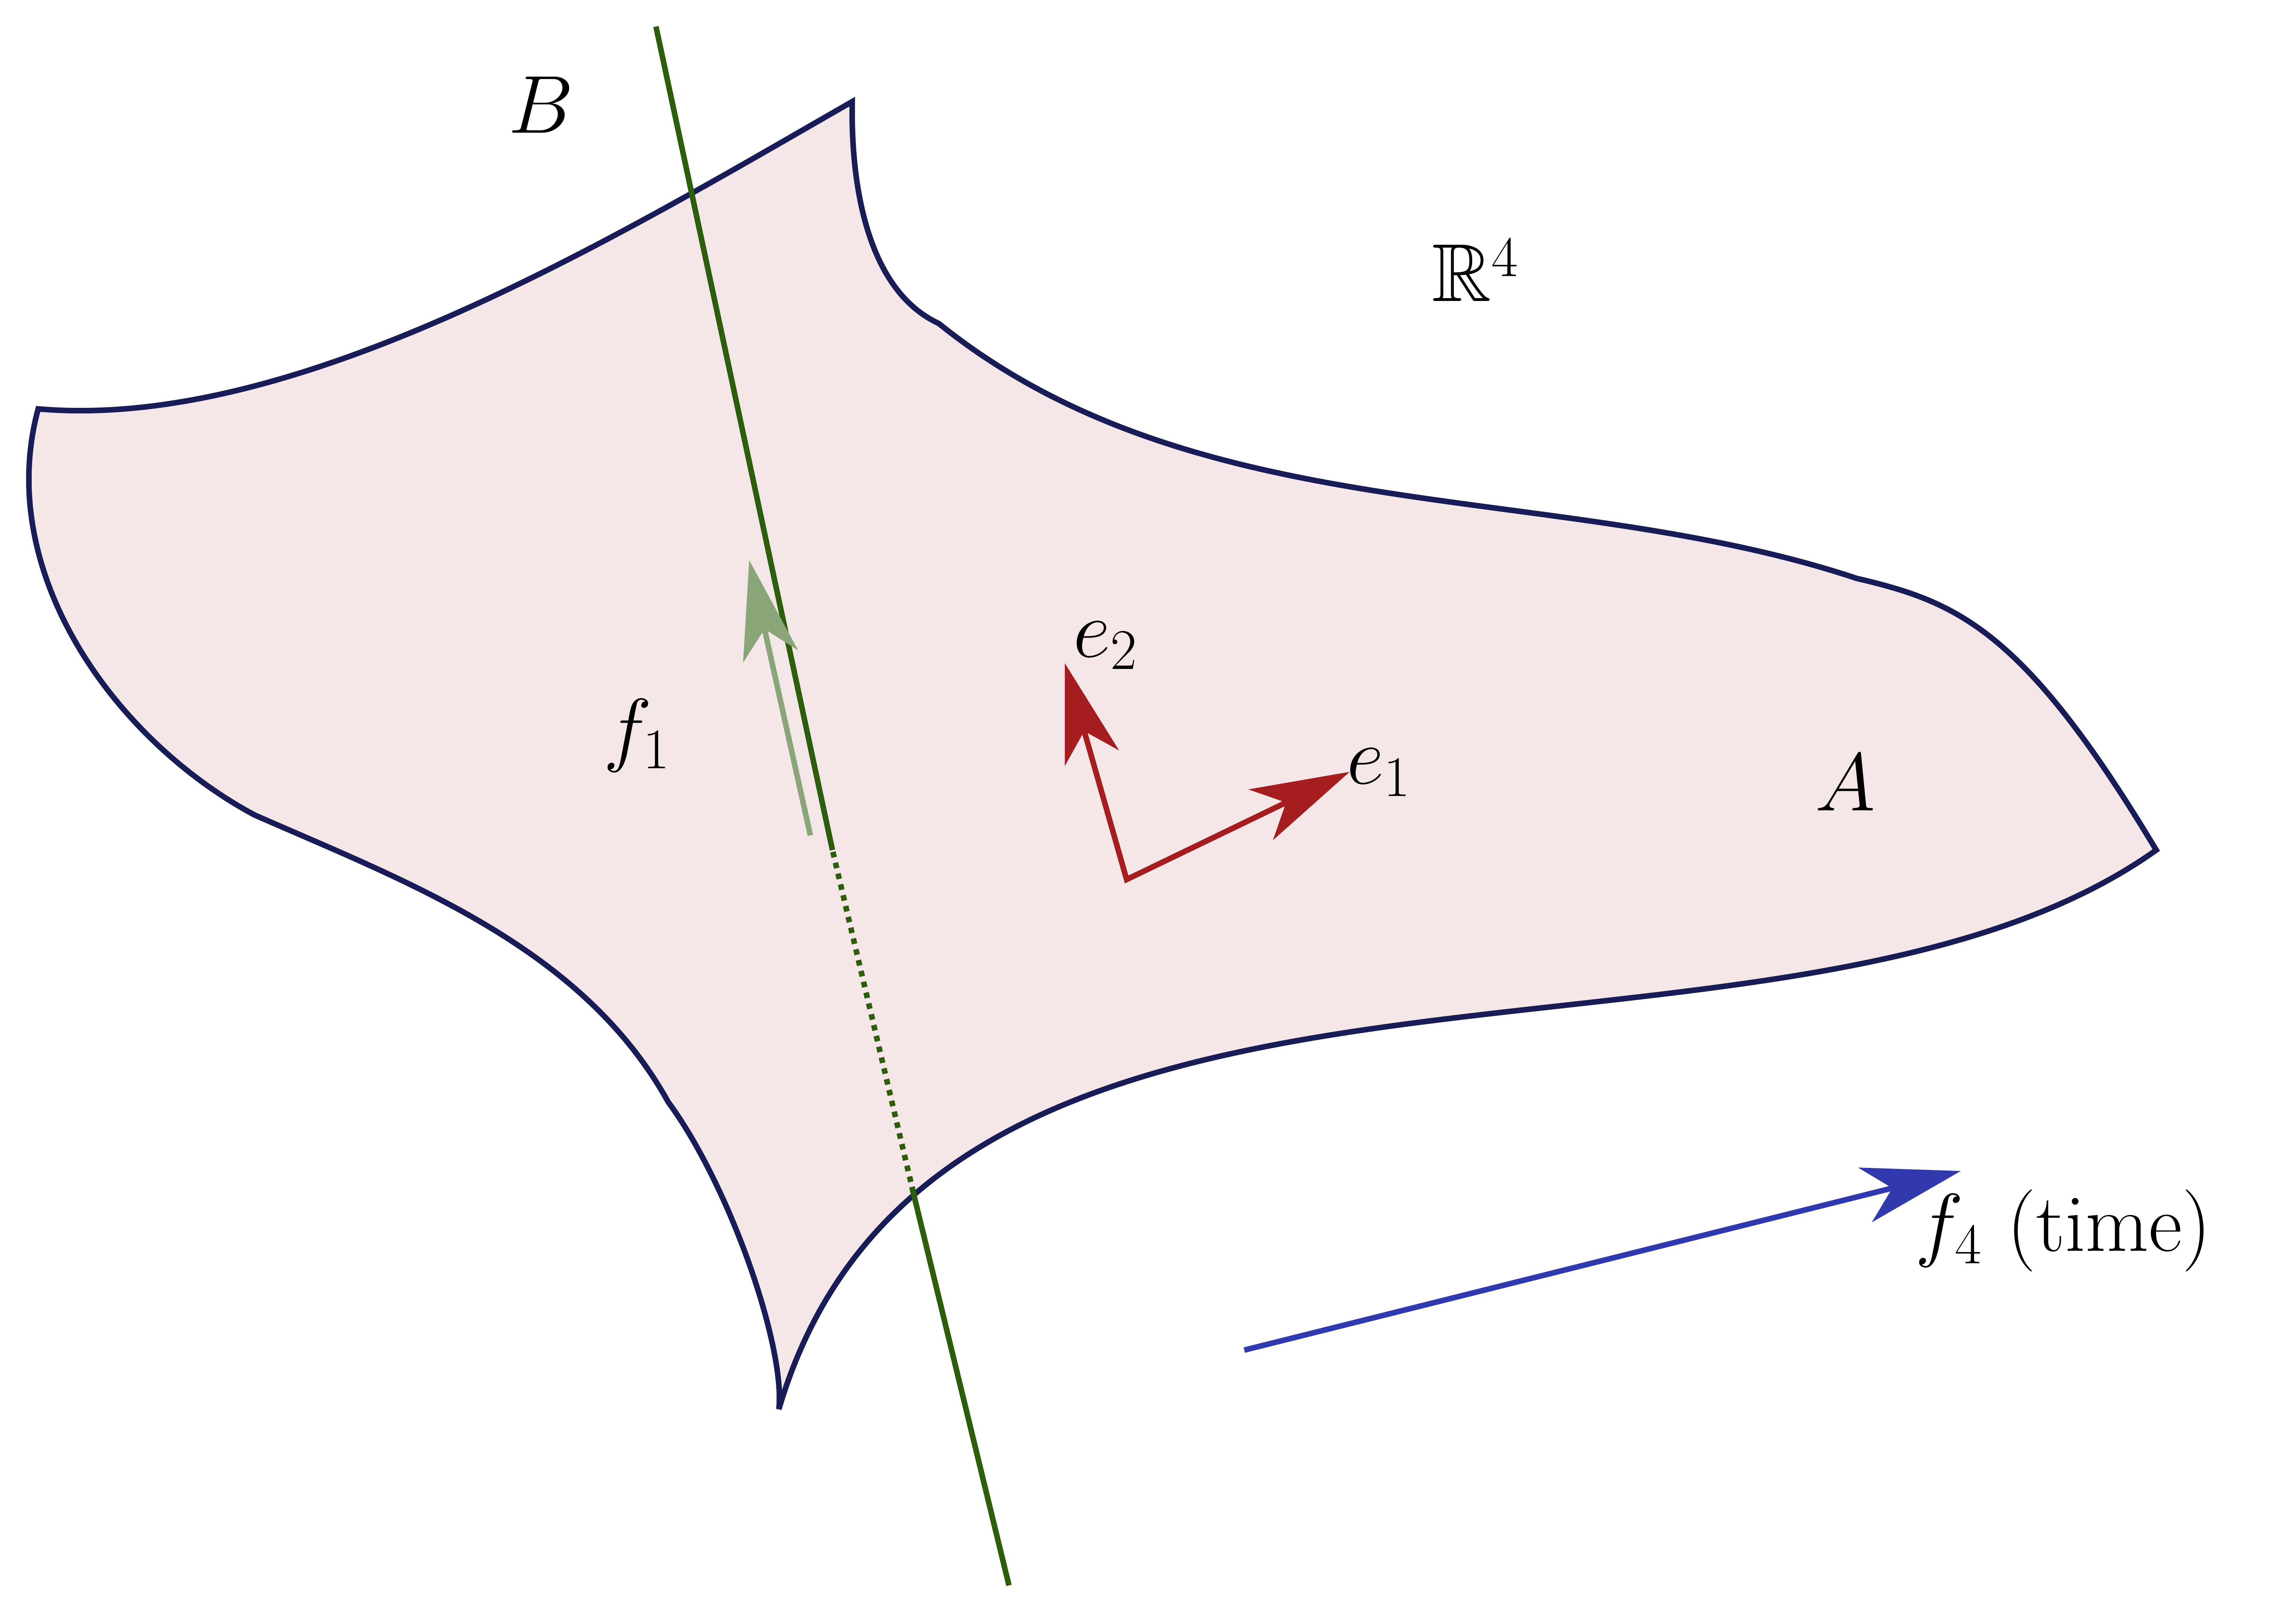
\includegraphics{figures/time_manifold_glitch_workaround.png}
\caption{Picking one basis element in the time direction}
\end{figure}

Here \(?\) is oriented in the ``forward time'' direction, and this is a
surface at time \(t=0\). Where \(A\cdot B = +1\), since
\(\left\{{ e_1, e_2, f_1, f_2 }\right\} = \left\{{ e_x, e_y, e_z, e_t }\right\}\)
is a oriented basis for \({\mathbb{R}}^4\). For \(?^2\), switching the
order of \(\alpha, \beta\) no longer yields an oriented basis, but in
this case it is \(?\) and \(A\cdot B = B \cdot A\). This is because
\begin{align*}
A \coloneqq
\begin{bmatrix}
0 &  1
\\
1 & 0 
\end{bmatrix}
\implies \det(A)
=-1 &&
\det 
\begin{bmatrix}
A &  
\\
 & A 
\end{bmatrix}
 = 1
.\end{align*}

\end{remark}

\begin{remark}

Let \(M^{2n}\) be an oriented manifold, then the cup product yields a
bilinear map
\(H^n(M; {\mathbb{Z}}) \otimes H^n(M; {\mathbb{Z}}) \to {\mathbb{Z}}\)
which is symmetric when \(n\) is odd and antisymmetric (or symplectic)
when \(n\) is even. This is a \textbf{perfect} (or \textbf{unimodular})
pairing (potentially after modding out by torsion) which realizes an
isomorphism:
\begin{align*}
\qty{ H^n(M; {\mathbb{Z}})/{\operatorname{tors}}}^\vee&\xrightarrow{\sim} H^n(M; {\mathbb{Z}})/{\operatorname{tors}}\\
\alpha \smile{\,\cdot\,}&\mapsfrom \alpha
,\end{align*}
where the LHS are linear functionals on cohomology.

\end{remark}

\begin{remark}

Recall the universal coefficients theorem:
\begin{align*}
H^i(X; {\mathbb{Z}})/{\operatorname{tors}}\cong \qty{ H_i(X; {\mathbb{Z}})/{\operatorname{tors}}}^\vee
.\end{align*}
The general theorem shows that
\(H^i(X; {\mathbb{Z}})_{\operatorname{tors}}= H_{i-1}(X; {\mathbb{Z}})_{\operatorname{tors}}\).

\end{remark}

\begin{remark}

Note that if \(M\) is an oriented 4-manifold, then

\begin{center}
\begin{tikzcd}
    && {\operatorname{tors}}& {\text{torsionfree}} &&&&& {\operatorname{tors}}& {\text{torsionfree}} \\
    {H^0} && 0 & {\mathbb{Z}}&&& {H_0} && 0 & {\mathbb{Z}}\\
    {H^1} && 0 & \textcolor{rgb,255:red,214;green,92;blue,92}{{\mathbb{Z}}^{\beta_1}} &&& {H_1} && A & \textcolor{rgb,255:red,214;green,92;blue,214}{{\mathbb{Z}}^{\beta_1}} \\
    {H^2} && A & \textcolor{rgb,255:red,92;green,92;blue,214}{{\mathbb{Z}}^{\beta_2}} & {} & {{}} & {H_2} && A & \textcolor{rgb,255:red,92;green,92;blue,214}{{\mathbb{Z}}^{\beta_2}} \\
    {H^3} && A & \textcolor{rgb,255:red,214;green,92;blue,214}{{\mathbb{Z}}^{\beta_1}} &&& {H_3} && 0 & \textcolor{rgb,255:red,214;green,92;blue,92}{{\mathbb{Z}}^{\beta_1}} \\
    {H^4} && 0 & {\mathbb{Z}}&&& {H_4} && 0 & {\mathbb{Z}}
    \arrow["PD", from=4-5, to=4-6]
\end{tikzcd}
\end{center}

In particular, if \(M\) is simply connected, then
\(H_1(M) = {\mathsf{Ab}}(\pi_1(M)) = 0\), which forces \(A = 0\) and
\(\beta_1 = 0\).

\end{remark}

\begin{definition}[Lattice]

A \textbf{lattice} is a finite-dimensional free
\({\mathbb{Z}}{\hbox{-}}\)module \(L\) together with a symmetric
bilinear form
\begin{align*}
\cdot: L^{\otimes 2} &\to {\mathbb{Z}}\\
\ell \otimes m &\mapsto \ell \cdot m
.\end{align*}
The lattice \((L, \cdot)\) is \textbf{unimodular} if and only if the
following map is an isomorphism:
\begin{align*}
L &\to L^\vee\\
\ell &\mapsto \ell \cdot ({\,\cdot\,})
.\end{align*}

\end{definition}

\begin{remark}

How to determine if a lattice is unimodular: take a basis
\(\left\{{ e_1, \cdots, e_n }\right\}\) of \(L\) and form the \emph{Gram
matrix}
\(M_{ij} \coloneqq( e_i \cdot e_j) \in \operatorname{Mat}(n\times n, {\mathbb{Z}})^{\operatorname{Sym}}\).
Then \((L, \cdot)\) is unimodular if and only if \(\det(M) = \pm 1\) if
and only if \(M ^{-1}\) is integral. In this case, the rows of
\(M ^{-1}\) will form a basis of the dual basis.

\end{remark}

\begin{definition}[?]

The \textbf{index} of a lattice is
\({\left\lvert { \det M} \right\rvert}\).

\end{definition}

\begin{exercise}[?]

Prove that
\({\left\lvert {\det M} \right\rvert} = {\left\lvert { L^\vee/ L } \right\rvert}\).

\end{exercise}

\begin{remark}

In general, for \(M^{4k}\), the \(H^{2k}/{\operatorname{tors}}\) is
unimodular. For \(M^{4k+2}\), the \(H^{2k+1}/{\operatorname{tors}}\) is
a unimodular \emph{symplectic} lattice, which is obtained by replacing
the word ``symmetric'' with ``antisymmetric'' everywhere above.

\end{remark}

\begin{example}[?]

For the torus, since the dimension is \(2 \pmod 4\), you get the
skew-symmetric matrix
\begin{align*}
\begin{bmatrix}
0  & 1
\\
-1 & 0
\end{bmatrix}
.\end{align*}

\todo[inline]{Check!}

\end{example}

\begin{definition}[?]

A lattice is \textbf{nondegenerate} if \(\det M \neq 0\).

\end{definition}

\begin{definition}[?]

The tensor product \(L \otimes_{\mathbb{Z}}{\mathbb{R}}\) is a vector
space with an \({\mathbb{R}}{\hbox{-}}\)valued symmetric bilinear form.
This allows extending the lattice from \({\mathbb{Z}}^n\) to
\({\mathbb{R}}^n\).

\end{definition}

\begin{remark}

If \((L, \cdot)\) is nondegenerate, then Gram-Schmidt will yield an
orthonormal basis \(\left\{{ v_i }\right\}\). The number of positive
norm vectors is an invariant, so we obtain \({\mathbb{R}}^{p, q}\) where
\(p\) is the number of \(+1\)s in the Gram matrix and \(q\) is the
number of \(-1\)s. The \textbf{signature} of \((L, {\,\cdot\,})\) is
\((p, q)\), or by abuse of notation \(p-q\). This is an invariant of the
4-manifold, as is the lattice itself
\(H^2(X; {\mathbb{Z}})/{\operatorname{tors}}\) equipped with the
intersection form.

\end{remark}

\begin{remark}

There is a perfect pairing called the \textbf{linking pairing}:

\begin{align*}
H^i(X; {\mathbb{Q}}/{\mathbb{Z}}) \otimes H^{n-i-1}(X; {\mathbb{Q}}/{\mathbb{Z}}) \to {\mathbb{Q}}/{\mathbb{Z}}
.\end{align*}

\begin{figure}
\centering
\resizebox{\columnwidth}{!}{%
\begin{tikzpicture}
\fontsize{44pt}{1em} 
\node (node_one) at (0,0) { \import{/home/zack/SparkleShare/github.com/Notes/Class_Notes/2021/Spring/FourManifolds/sections/figures}{2021-02-03_14-43.pdf_tex} };
\end{tikzpicture}
}
\end{figure}

\end{remark}

\begin{remark}

\(A \cdot B \coloneqq\sum_{p\in A \cap B} \operatorname{sgn}_p(A, B)\),
where \(A \pitchfork B\) and this turns out to be equal to the cup
product. This works for topological manifolds -- but there are no
tangent spaces there, so taking oriented bases doesn't work so well! You
can also view
\begin{align*}
[A] \smile[\omega] = \int_A \omega
.\end{align*}

\end{remark}

\hypertarget{friday-february-05}{%
\section{Friday, February 05}\label{friday-february-05}}

\begin{remark}

Recall that a lattice is \textbf{unimodular} if the map
\(L\to L^\vee\coloneqq{\operatorname{Hom}}(L, {\mathbb{Z}})\) is an
isomorphism, where \(\ell \mapsto \ell \cdot ({\,\cdot\,})\). To check
this, it suffices to check if the Gram matrix \(M\) of a basis
\(\left\{{e_i}\right\}\) satisfies
\({\left\lvert { \det M } \right\rvert} = 1\).

\end{remark}

\begin{example}[Determinant 1 Integer Matrices]

The matrices \([1]\) and \([-1]\) correspond to the lattice
\({\mathbb{Z}}e\) where either \(e^2 \coloneqq e\cdot e = 1\) or
\(e^2 = -1\). If \(M_1, M_2\) both have absolute determinant \(1\), then
so does
\begin{align*}
\begin{bmatrix}
M_1 & 0 
\\
0 & M_2
\end{bmatrix}
.\end{align*}

So if \(L_1, L_2\) are unimodular, then taking an orthogonal sum
\(L_1 \oplus L_2\) also yields a unimodular lattice. So this yields
diagonal matrices with \(p\) copies of \(+1\) and \(q\) copies of
\(-1\). This is referred to as \(rm{1}_{p, q}\), and is an \emph{odd}
unimodular lattice of signature \((p, q)\) (after passing to
\({\mathbb{R}}\)). Here \emph{odd} means that there exists a \(v\in L\)
such that \(v^2\) is odd.

\end{example}

\begin{example}[Even unimodular lattices]

An even lattice must have no vectors of odd norm, so all of the diagonal
elements are in \(2{\mathbb{Z}}\). This is because
\((\sum n_i e_i)^2 = \sum_i n_i^2 e_i^2 + \sum_{i<j} 2 n_i, n_j e_i \cdot e_j\).
Note that the matrix must be symmetric, and one example that works is
\begin{align*}
\begin{bmatrix}
0 & 1 
\\
1 & 0
\end{bmatrix}
.\end{align*}
We'll refer to this lattice as \(H\), sometimes referred to as the
\emph{hyperbolic cell} or \emph{hyperbolic plane}.

\end{example}

\begin{example}[A harder even unimodular lattice]

This is built from the \(E_8\) Dynkin diagram:

\begin{center}
\begin{tikzcd}
    &&&& {\bullet_{e_8}} \\
    {\bullet_{e_7}} & {\bullet_{e_6}} & {\bullet_{e_5}} & {\bullet_{e_4}} & {\bullet_{e_3}} & {\bullet_{e_2}} & {\bullet_{e_1}}
    \arrow[no head, from=2-1, to=2-2]
    \arrow[no head, from=2-2, to=2-3]
    \arrow[no head, from=2-3, to=2-4]
    \arrow[no head, from=2-4, to=2-5]
    \arrow[no head, from=2-5, to=1-5]
    \arrow[no head, from=2-5, to=2-6]
    \arrow[no head, from=2-6, to=2-7]
\end{tikzcd}
\end{center}

The rule here is
\begin{align*}
e_i \cdot e_j = 
\begin{cases}
-2  & i =  j
\\
1 & e_i \to e_j \\
0 & \text{if not connected}.
\end{cases}
\end{align*}
So for example, \(e_2 \cdot e_6 = 0, e_1 \cdot e_3 = 1, e_2^2 = -2\).
You can check that \(\det(e_i \cdot e_j) = 1\), and this is referred to
as the \(E_8\) lattice. This is of signature \((0, 8)\), and it's
negative definite if and only if \(v^2 < 0\) for all \(v\neq 0\). One
can also negate the intersection form to define \(-E_8\). Note that any
simply-laced Dynkin diagram yields some lattice. For example, \(E_{10}\)
is unimodular of signature \((1, 9)\), and it turns out that
\(E_{10} \cong E_8 \oplus H\).

\end{example}

\begin{definition}[?]

Take
\begin{align*} 
\mathbf{II}_{a, a+8b} \coloneqq\bigoplus_{i=1}^a H \oplus \bigoplus_{j=1}^b E_8 
,\end{align*}
which is an even unimodular lattice since the diagonal entries are all
\(-2\), and using the fact that the signature is additive, is of
signature \((a, a+8b)\). Similarly,
\begin{align*} 
\mathbf{II}_{a+8b, a} \coloneqq\bigoplus_{i=1}^a H \oplus \bigoplus_{j=1}^b (-E_8) 
,\end{align*}
which is again even and unimodular.

\end{definition}

\begin{remark}

Thus

\begin{itemize}
\tightlist
\item
  \(\mathbf{I}_{p, q}\) is odd, unimodular, of signature \((p, q)\).
\item
  \(\mathbf{II}_{p, q}\) is even, unimodular, of signature \((p, q)\)
  only for \(p \equiv q \pmod 8\).
\end{itemize}

\end{remark}

\begin{theorem}[Serre]

Every unimodular lattice which is not positive or negative definite is
isomorphic to either \(\mathbf{I}_{p, q}\) or \(\mathbf{II}_{p, q}\)
with \(8\mathrel{\Big|}p-q\).

\end{theorem}

\begin{remark}

So there are obstructions to the existence of even unimodular lattices.
Other than that, the number of (say) positive definite even unimodular
lattices is

\begin{longtable}[]{@{}ll@{}}
\toprule
Dimension & Number of Lattices \\ \addlinespace
\midrule
\endhead
8 & 1: \(E_8\) \\ \addlinespace
16 & 2: \(E_8^{\oplus 2}, D_{16}^+\) \\ \addlinespace
24 & 24: The Neimeir lattices (e.g.~the Leech lattice) \\ \addlinespace
32 & \textgreater{}\(8\times 10^{16}\)!!!! \\ \addlinespace
\bottomrule
\end{longtable}

Note that the signature of a definite lattice must be divisible by 8.

\end{remark}

\begin{remark}

There is an isometry: \(f: E_8 \to E_8\) where \(f\in O(E_8)\), the
linear maps preserving the intersection form (i.e.~the Weyl group
\(W(E_8)\), given by \(v\mapsto v + (v, e_i) e_i\). The Leech lattice
also shows up in the sphere packing problems for dimensions
\(2,4,8,24\). See Hale's theorem / Kepler conjecture for dimension 3!
This uses an identification of \(L\) as a subset of \({\mathbb{R}}^n\),
namely \(L \otimes_{\mathbb{Z}}{\mathbb{R}}\cong {\mathbb{R}}^{24}\) for
example, and the map \(L \hookrightarrow({\mathbb{R}}^{24}, \cdot)\) is
an isometric embedding into \({\mathbb{R}}^n\) with the standard form.
Connection to classification of Lie groups: root lattices.

\end{remark}

\begin{remark}

If \(M^4\) is a compact oriented 4-manifold and if the intersection form
on \(H^2(M; {\mathbb{Z}})\) is indefinite, then the only invariants we
can extract from that associated lattice are

\begin{itemize}
\tightlist
\item
  Whether it's even or odd, and
\item
  Its signature
\end{itemize}

If the lattice is even, then the signature satisfies
\(8\mathrel{\Big|}p-q\). So Poincaré duality forces unimodularity, and
then there are further number-theoretic restrictions. E.g. this
prohibits \(\beta_2 =7\), since then the signature couldn't possibly be
8 if the intersection form is even.

\end{remark}

\hypertarget{characteristic-classes}{%
\subsection{Characteristic Classes}\label{characteristic-classes}}

\begin{definition}[?]

Let \(G\) be a topological group, then a \textbf{classifying space}
\(EG\) is a contractible topological space admitting a free continuous
\(G{\hbox{-}}\)action with a ``nice'' quotient.

\end{definition}

\begin{remark}

Thus there is a map \(EG \to BG \coloneqq EG/G\) which has the structure
of a principal \(G{\hbox{-}}\)bundle.

\begin{figure}
\centering
\resizebox{\columnwidth}{!}{%
\begin{tikzpicture}
\fontsize{40pt}{1em} 
\node (node_one) at (0,0) { \import{/home/zack/SparkleShare/github.com/Notes/Class_Notes/2021/Spring/FourManifolds/sections/figures}{2021-02-05_14-37.pdf_tex} };
\end{tikzpicture}
}
\end{figure}

Here we use a point \(p\) depending on \(U\) in an orbit to identify
orbits \(g\cdot p\) with \(g\), and we want to take transverse slices to
get local trivializations of \(U\in BG\). It suffices to know where
\(\pi ^{-1} (U) \cong U \times G\), and it suffices to consider
\(U \times\left\{{e}\right\}\). Moreover, \(EG\to BG\) is a universal
principal \(G{\hbox{-}}\)bundle in the sense that if \(P\to X\) is a
universal \(G{\hbox{-}}\)bundle, there is an \(f:X\to BG\).

\begin{center}
\begin{tikzcd}
    P && EG \\
    \\
    X && BG
    \arrow[from=1-1, to=3-1]
    \arrow["f", from=3-1, to=3-3]
    \arrow[from=1-3, to=3-3]
    \arrow[dashed, from=1-1, to=1-3]
\end{tikzcd}
\end{center}

\begin{quote}
\href{https://q.uiver.app/?q=WzAsNCxbMCwyLCJYIl0sWzIsMCwiRUciXSxbMiwyLCJCRyJdLFswLDAsIlAiXSxbMywwXSxbMCwyLCJmIl0sWzEsMl0sWzMsMSwiIiwyLHsic3R5bGUiOnsiYm9keSI6eyJuYW1lIjoiZGFzaGVkIn19fV1d}{Link
to Diagram}
\end{quote}

Here bundles will be classified by homotopy classes of \(f\), so
\begin{align*}
\left\{{\text{Principal $G{\hbox{-}}$bundles} {}_{/ X} }\right\} \rightleftharpoons[X, BG]
.\end{align*}

\end{remark}

\begin{warnings}

This only works for paracompact Hausdorff spaces! The line
\({\mathbb{R}}\) with the doubled origin is a counterexample, consider
complex line bundles.

\end{warnings}

\todo[inline]{Revisit this last section, had to clarify a few things for myself!}

\hypertarget{monday-february-08}{%
\section{Monday, February 08}\label{monday-february-08}}

Last time: \(BG\) and \(EG\). See Milnor and Stasheff.

\begin{example}[?]

Let
\(G \coloneqq\operatorname{GL}_n({\mathbb{R}}) = {\mathbb{R}}^{\times}\),
then we can take
\begin{align*}
EG = {\mathbb{R}}^{\infty } \coloneqq\left\{{ (a_1, a_2, \cdots ) {~\mathrel{\Big|}~}a_i \in {\mathbb{R}}, a_{i\gg 0} = 0, a_i \text{ not all zero } }\right\}
.\end{align*}
Then \({\mathbb{R}}^{\times}\) acts on \(EG\) by scaling, and we can
take the quotient
\({\mathbb{R}}^{\infty } \setminus\left\{{0}\right\}/ {\mathbb{R}}^{\times}\),
where \(\mathbf{a} \sim \lambda \mathbf{a}\) for all
\(\lambda \in {\mathbb{R}}^{\times}\). This yields
\({\mathbb{RP}}^{\infty }\) as the quotient. You can check that \(E_G\)
is contractible: it suffices to show that
\(S^{\infty } \coloneqq\left\{{ \sum {\left\lvert {a_i} \right\rvert} = 1 }\right\}\)
is contractible. This works by decreasing the last nonzero coordinate
and increasing the first coordinate correspondingly. Moreover, local
lifts exist, so we can identify
\({\mathbb{RP}}^{\infty } \cong B{\mathbb{R}}^{\times}= BG\). Similarly
\(BC^{\times}\cong {\mathbb{CP}}^{\infty }\) with
\(E{\mathbb{C}}^{\times}\coloneqq{\mathbb{C}}^{\infty } \setminus\left\{{0}\right\}\).

\end{example}

\begin{example}[?]

Consider \(G = \operatorname{GL}_n({\mathbb{R}})\). It turns out that
\(BG = {\operatorname{Gr}}(d, {\mathbb{R}}^{\infty })\), which is the
set of linear subspaces of \({\mathbb{R}}^{\infty }\) of dimension
\(d\). This is spanned by \(d\) vectors \(\left\{{e_ i}\right\}\) in
some large enough \({\mathbb{R}}^N \subseteq {\mathbb{R}}^{\infty }\),
since we can take \(N\) to be the largest nonvanishing coordinate and
include all of the vectors into \({\mathbb{R}}^{\infty }\) by setting
\(a_{> N} = 0\). For any
\(L \in {\operatorname{Gr}}_d({\mathbb{R}}^{\infty })\), since
\({\mathbb{R}}^d\) has a standard basis, there is a natural
\(\operatorname{GL}_d\) torsor: the set of ordered bases of linear
subspaces. So define
\begin{align*}
EG \coloneqq\left\{{ \text{bases of linear subspaces } L \in {\operatorname{Gr}}_d({\mathbb{R}}^{\infty }) }\right\}
,\end{align*}
then any \(A\in \operatorname{GL}_d({\mathbb{R}})\) acts on \(EG\) by
sending
\((L, \left\{{e_i}\right\}) \mapsto (L, \left\{{ Le_i}\right\} )\). We
can identify \(EG\) as \(d{\hbox{-}}\)tuples of linearly independent
elements of \({\mathbb{R}}^{\infty }\), and there is a map
\begin{align*}
EG &\to BG \\
\left\{{e_i}\right\} &\mapsto {\operatorname{span}}_{\mathbb{R}}\left\{{e_i}\right\}
.\end{align*}
Thus there is a universal vector bundle over \(BGL_d\):

\begin{center}
\begin{tikzcd}
\mathcal{E}_L \coloneqq L 
  \ar[r] 
& 
\mathcal{E} 
  \ar[d] 
\\
& 
BGL_d
\end{tikzcd}
\end{center}

So \(\mathcal{E} \subseteq BGL_d \times{\mathbb{R}}^{\infty }\), where
we can define
\(\mathcal{E} \coloneqq\left\{{(L, p) {~\mathrel{\Big|}~}p\in L}\right\}\).
In this case, \(EG = {\operatorname{Frame}}( \mathcal{E})\) is the frame
bundle of this universal bundle. The same setup applies for
\(G \coloneqq\operatorname{GL}_d({\mathbb{C}})\), except we take
\({\operatorname{Gr}}_d({\mathbb{C}}^{\infty })\).

\end{example}

\begin{example}[?]

Consider \(G = O_d\), the set of orthogonal transformations of
\({\mathbb{R}}^d\) with the standard bilinear form, and \(U_d\) the set
of unitary such transformations. To be explicit:
\begin{align*}
U_d \coloneqq\left\{{ A \in \operatorname{Mat}(d \times d, {\mathbb{C}}) {~\mathrel{\Big|}~}{\left\langle {Av},~{Av} \right\rangle} = {\left\langle {v},~{v} \right\rangle} }\right\}
,\end{align*}
where
\begin{align*}
{\left\langle { {\left[ {v_1, \cdots, v_n} \right]}},~{{\left[ {v_1, \cdots, v_n } \right]} } \right\rangle} = \sum {\left\lvert {v_i} \right\rvert}^2
.\end{align*}
Alternatively, \(A^t A = I\) for \(O_d\) and
\({\overline{{A^t}}} A = I\) for \(U_d\). In this case,
\(BO_d = {\operatorname{Gr}}_d( {\mathbb{R}}^{\infty } )\) and
\(BU_d = {\operatorname{Gr}}_d( {\mathbb{C}}^{ \infty })\), but we'll
make the fibers smaller: set the fiber over \(L\) to be
\begin{align*}
(EO_d)_L \coloneqq\left\{{ \text{orthogonal frames of } L }\right\}
\end{align*}
and similarly \((EU_d)_L\) the unitary frames of \(L\). That there are
related comes from the fact that \(\operatorname{GL}_d\) retracts onto
\(O_d\) using the Gram-Schmidt procedure.

\end{example}

\begin{remark}

Recall that there is a bijective correspondence
\begin{align*}
\left\{{\substack{
  \text{Principal $G{\hbox{-}}$ bundles}
  \\ \text{on } X
}}\right\}
&\rightleftharpoons
  [X, BG]
\end{align*}
and there is also a correspondence
\begin{align*}
\left\{{\substack{
  \text{Principal $\operatorname{GL}_d{\hbox{-}}$bundles }\\
  \text{on } X
}}\right\}
&\rightleftharpoons
\left\{{\substack{
  \text{Principal ${\mathcal{O}}_d{\hbox{-}}$bundles } \\
  \text{on } X
}}\right\}
\end{align*}
Using the associated bundle construction, on the LHS we obtain vector
bundles \(\mathcal{E}\to X\) of rank \(d\), and on the RHS we have
bundles with a metric. In local trivializations
\(U \times{\mathbb{R}}^d \to {\mathbb{R}}^d\), the metric is the
standard one on \({\mathbb{R}}^d\). This is referred to as a
\textbf{reduction of structure group}, i.e.~a principal
\(\operatorname{GL}_d\) bundle admits possibly different trivializations
for which the transition functions lie in the subgroup \(O_d\).

\end{remark}

\begin{example}[?]

Given any trivial principal \(G{\hbox{-}}\)bundle, it has a reduction of
structure group to the trivial group. But the fact that the bundle is
trivial may not be obvious.

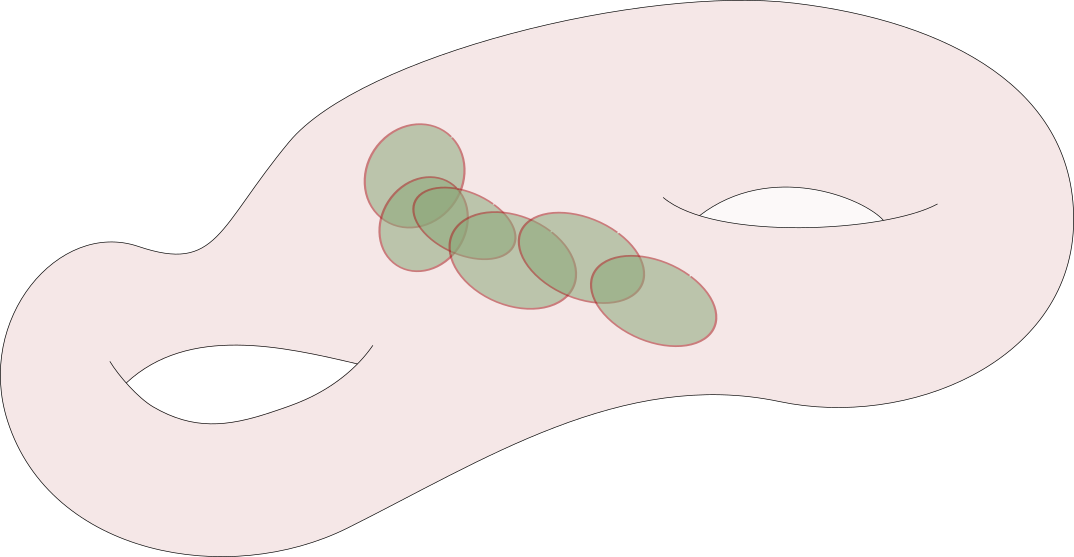
\includegraphics{figures/forbidden_donut.png}

\end{example}

\begin{remark}

We want to compute \(H^*(BU_d; {\mathbb{Z}})\). Why is this important?
Given any complex vector bundle \(\mathcal{E}\to X\) there is an
associated principal \(U_d\) bundle by choosing a metric, so we get a
homotopy class \([X, BU_d]\). Given any \(f\in [X, BU_d]\) and any
\(\alpha\in H^k(BU_d; {\mathbb{Z}})\), we can take the pullback
\(f^* \alpha \in H^k(X; {\mathbb{Z}})\), which are \textbf{Chern
classes}.

\end{remark}

\begin{exercise}[?]

Show that \(H^*(BU_d; {\mathbb{Z}})\) stabilizes as \(d\to \infty\) to
an infinitely generated polynomial ring
\({\mathbb{Z}}[c_1, c_2, \cdots]\) with each \(c_i\) in cohomological
degree \(2i\), so \(c_i \in H^{2i}(BU_d, {\mathbb{Z}})\).

\end{exercise}

\begin{definition}[?]

There is a map \(BU_{d-1} \to BU_d\), which we can identify as
\begin{align*}
{\operatorname{Gr}}_{d-1}(C^{\infty }) &\to {\operatorname{Gr}}_d({\mathbb{C}}^{\infty }) \\
\left\{{v_1, \cdots, v_{d-1}}\right\} &\mapsto {\operatorname{span}}\left\{{ (1, 0, 0, \cdots), sv_1, \cdots, sv_{d-1} }\right\}
.\end{align*}
This is defined by sending a basis where
\(s: {\mathbb{C}}^{\infty } \to {\mathbb{C}}^{\infty}\) is the map that
shifts every coordinate to the right by one.

\todo[inline]{
  Question: does ${\operatorname{Gr}}_d({\mathbb{C}}^{\infty})$ deformation retract onto the image of this map?
}

This will yield a fiber sequence
\begin{align*}
S^{2d-1} \to BU_{d-1} \to BU_d
\end{align*}
and using connectedness of the sphere and the LES in homotopy this will
identify
\begin{align*}
H^*(BU_d) = H^*(BU_{d-1})[c_d] && \text{where } c_d \in H^{2d}(BU_d)
.\end{align*}
The \textbf{Chern class} of a vector bundle \(\mathcal{E}\) , denoted
\(c_k( \mathcal{E} )\), will be defined as the pullback \(f^* c_k\).

\end{definition}

\hypertarget{wednesday-february-10}{%
\section{Wednesday, February 10}\label{wednesday-february-10}}

\begin{theorem}[?]

As \(n\to \infty\), we have
\begin{align*}
H^*(BO_n, {\mathbb{Z}}/2{\mathbb{Z}}) = {\mathbb{Z}}/2{\mathbb{Z}}[w_1, w_2, \cdots]
&& w_i \in H^i
.\end{align*}

\end{theorem}

\begin{definition}[?]

Given any principal \(O_n{\hbox{-}}\)bundle \(P\to X\), there is an
induced map \(X \xrightarrow{f} BO_n\), so we can pull back the above
generators to define the \textbf{Stiefel-Whitney classes} \(f^* w_i\).

\end{definition}

\begin{remark}

If \(P \coloneqq{\operatorname{OFrame}}TX\), then \(f^* w_1\) measures
whether \(X\) has an orientation, i.e.~\(f^* w_1 = 0 \iff X\) can be
oriented. We also have \(f^* w_i(P) = w_i( \mathcal{E} )\) where
\(P = {\operatorname{OFrame}}( \mathcal{E} )\). In general, we'll just
write \(w_i\) for Stiefel-Whitney classes and \(c_i\) for Chern classes.

\end{remark}

\begin{definition}[Pontryagin Classes]

The \textbf{Pontryagin classes} of a real vector bundle \(\mathcal{E}\)
are defined as
\begin{align*}
p_i( \mathcal{E} ) = (-1)^i c_{2i}( \mathcal{E} \otimes_{\mathbb{R}}{\mathbb{C}})
.\end{align*}
Note that the complexified bundle above is a complex vector bundle with
the same transition functions as \(\mathcal{E}\), but has a reduction of
structure group from \(\operatorname{GL}_n({\mathbb{C}})\) to
\(\operatorname{GL}_n({\mathbb{R}})\).

\end{definition}

\begin{observation}

\({\mathbb{RP}}^{\infty }\) and \({\mathbb{CP}}^{\infty }\) are examples
of \(K(\pi, n)\) spaces, which are the unique-up-to-homotopy spaces
defined by
\begin{align*}
\pi_k K (\pi, n) = 
\begin{cases}
\pi &  k=n
\\
0 & \text{else}.
\end{cases}
\end{align*}

\end{observation}

\begin{theorem}[Brown Representability]

\begin{align*}
H^n(X; \pi) \cong [X, K( \pi, n) ]
.\end{align*}

\end{theorem}

\begin{example}[?]

\begin{align*}
[X, {\mathbb{RP}}^{\infty } ] &\cong H^1(X; {\mathbb{Z}}/2{\mathbb{Z}}) \\
[X, {\mathbb{CP}}^{\infty } ] &\cong H^2(X; {\mathbb{Z}})
.\end{align*}

\end{example}

\begin{proposition}[?]

There is a correspondence
\begin{align*}
\left\{{\substack{
  \text{Complex line bundles}
}}\right\}
\rightleftharpoons
[X, {\mathbb{CP}}^{\infty }] = [X, BC^{\times}]
\rightleftharpoons
H^2(X; {\mathbb{Z}})
\end{align*}
Importantly, note that for \(X \in {\mathsf{Mfd}}_{\mathbb{C}}\),
\(H^2(X; {\mathbb{Z}})\) measures \emph{smooth} complex line bundles and
not holomorphic bundles.

\end{proposition}

\begin{proof}[?]

We'll take an alternate direct proof. Consider the exponential exact
sequence on \(X\):
\begin{align*}
0 \to \underline{Z} \to {\mathcal{O}}\xrightarrow{\exp} {\mathcal{O}}^{\times}
.\end{align*}
Note that \(\underline{{\mathbb{Z}}}\) consists of locally constant
\({\mathbb{Z}}{\hbox{-}}\)valued functions, \({\mathcal{O}}\) consists
of smooth functions, and \({\mathcal{O}}^{\times}\) are ???.

\todo[inline]{Can't read screenshot! :(}

This yields a LES in homology:

\begin{center}
\begin{tikzcd}
    {H^0(X; \underline{{\mathbb{Z}}})} && {H^0(X; {\mathcal{O}})} && {H^0(X; {\mathcal{O}}^{\times})} \\
    \\
    {H^1(X; \underline{{\mathbb{Z}}})} && \textcolor{rgb,255:red,214;green,92;blue,92}{H^1(X; {\mathcal{O}})} && {H^1(X; {\mathcal{O}}^{\times})} \\
    \\
    {H^2(X; \underline{{\mathbb{Z}}})} && \textcolor{rgb,255:red,214;green,92;blue,92}{H^2(X; {\mathcal{O}})} && {H^2(X; {\mathcal{O}}^{\times})}
    \arrow[from=1-1, to=1-3]
    \arrow[from=1-3, to=1-5]
    \arrow[from=1-5, to=3-1, out=0, in=180]
    \arrow[from=3-1, to=3-3]
    \arrow[from=3-3, to=3-5]
    \arrow[from=3-5, to=5-1, out=0, in=180]
    \arrow[from=5-1, to=5-3]
    \arrow[from=5-3, to=5-5]
\end{tikzcd}
\end{center}

\begin{quote}
\href{https://q.uiver.app/?q=WzAsOSxbMCwwLCJIXjAoWDsgXFxjb25zdGFudHtcXFpafSkiXSxbMCwyLCJIXjEoWDsgXFxjb25zdGFudHtcXFpafSkiXSxbMCw0LCJIXjIoWDsgXFxjb25zdGFudHtcXFpafSkiXSxbMiwwLCJIXjAoWDsgXFxPTykiXSxbMiwyLCJIXjEoWDsgXFxPTykiLFswLDYwLDYwLDFdXSxbMiw0LCJIXjIoWDsgXFxPTykiLFswLDYwLDYwLDFdXSxbNCwwLCJIXjAoWDsgXFxPT1xcdW5pdHMpIl0sWzQsMiwiSF4xKFg7IFxcT09cXHVuaXRzKSJdLFs0LDQsIkheMihYOyBcXE9PXFx1bml0cykiXSxbMCwzXSxbMyw2XSxbNiwxXSxbMSw0XSxbNCw3XSxbNywyXSxbMiw1XSxbNSw4XV0=}{Link
to Diagram}
\end{quote}

Since \({\mathcal{O}}\) admits a partition of unity,
\(H^{>0}(X; {\mathcal{O}}) = 0\) and all of the red terms vanish. For
complex line bundles \(L\),
\(H^1(X, {\mathcal{O}}^{\times}) \cong H^2(X; {\mathbb{Z}})\). Taking a
local trivialization
\({ \left.{{L}} \right|_{{U}} } \cong U \times{\mathbb{C}}\), we obtain
transition functions
\begin{align*}
t_{UV} \in C^{\infty }(U \cap V, \operatorname{GL}_1({\mathbb{C}}) )
\end{align*}
where we can identify
\(\operatorname{GL}_1({\mathbb{C}}) \cong {\mathbb{C}}^{\times}\). We
then have
\begin{align*}
(t_{U_{ij}}) \in \prod_{i < j} {\mathcal{O}}^{\times}(U_i \cap U_j) = C^1(X; {\mathcal{O}}^{\times})
.\end{align*}
Moreover,
\begin{align*}
\qty{ 
t_{U_{ij}}
t_{U_{ik}} ^{-1}
t_{U_{jk}}
}_{i,j,k} 
= {{\partial}}( t_{U_{ij} } ) _{i, j} = 0
,\end{align*}
since transitions functions satisfy the cocycle condition. So in fact
\((t_{U_{ij}}) \in Z^1(X; {\mathcal{O}}^{\times}) = \ker {{\partial}}^1\),
and we can take its equivalence class
\([ ( t_{U_{ij} } ) ] \in H^1(X; {\mathcal{O}}^{\times}) = \ker {{\partial}}^1 / \operatorname{im}{{\partial}}^0\).
Changing trivializations by some
\(s_i \in \prod_i {\mathcal{O}}^{\times}(U_i)\) yields a composition
which is a different trivialization of the same bundle:

\begin{center}
\begin{tikzcd}
    {{ \left.{{L}} \right|_{{U_i}} }} && {U_i \times{\mathbb{C}}} &&& {U_i \times{\mathbb{C}}}
    \arrow["{h_i}", from=1-1, to=1-3]
    \arrow["{\cdot s_i}", from=1-3, to=1-6]
    \arrow[curve={height=30pt}, from=1-1, to=1-6]
\end{tikzcd}
\end{center}

\begin{quote}
\href{https://q.uiver.app/?q=WzAsMyxbMCwwLCJcXHJve0x9e1VfaX0iXSxbMiwwLCJVX2kgXFxjcm9zcyBcXENDIl0sWzUsMCwiVV9pIFxcY3Jvc3MgXFxDQyJdLFswLDEsImhfaSJdLFsxLDIsIlxcY2RvdCBzX2kiXSxbMCwyLCIiLDIseyJjdXJ2ZSI6NX1dXQ==}{Link
to Diagram}
\end{quote}

So the \((t_{ U_{ij}}\) change \emph{exactly} by an
\({{\partial}}^0( s_i)\). Thus the following map is well-defined:
\begin{align*}
L \mapsto [ (t_{U_{ij}} ) ] \in H^1(X; {\mathcal{O}}^{\times})
.\end{align*}

There is another construction of the map
\begin{align*}
\left\{{L}\right\} &\to H^2(X; {\mathbb{Z}}) \\
L &\mapsto c_1(L)
.\end{align*}
Take a smooth section of \(L\) and \(s\in H^0(X; L)\) that intersects an
\({\mathcal{O}}{\hbox{-}}\)section of \(L\) transversely. Then
\begin{align*}
V(s) \coloneqq\left\{{ x\in X {~\mathrel{\Big|}~}s(x) = 0 }\right\}
\end{align*}
is a submanifold of real codimension 2 in \(X\), and
\(c_1(L) = [ V(s) ] \in H^2(X; {\mathbb{Z}})\).

\end{proof}

\begin{theorem}[Splitting Principle for Complex Vector Bundles]

\envlist

\begin{enumerate}
\def\labelenumi{\arabic{enumi}.}
\item
  Suppose that \(\mathcal{E} = \bigoplus_{i=1}^r L_i\) and let
  \(c(\mathcal{E}) \coloneqq\sum c_i(\mathcal{E}\). Then
  \begin{align*}
    c(\mathcal{E}) = \prod_{i=1}^r \qty{ 1 + c_i (L_i) }
    .\end{align*}
\item
  Given any vector bundle \(\mathcal{E} \to X\), there exists some \(Y\)
  and a map \(Y\to X\) such that
  \(f^*: H^k(X; {\mathbb{Z}}) \hookrightarrow H^k(Y; {\mathbb{Z}})\) is
  injective and \(f^* \mathcal{E} = \bigoplus_{i=1}^r L_i\).
\end{enumerate}

\end{theorem}

\begin{slogan}

To verify any identities on characteristic classes, it suffices to prove
them in the case where \(\mathcal{E}\) splits into a direct sum of line
bundles.

\end{slogan}

\begin{example}[?]

\begin{align*}
c( \mathcal{E} \oplus \mathcal{F}) = c( \mathcal{E} ) c( \mathcal{F} )
.\end{align*}
To prove this, apply the splitting principle. Choose \(Y, Y'\) splitting
\(\mathcal{E}, \mathcal{E}'\) respectively, this produces a space \(Z\)
and a map \(f:Z\to X\) where both split. We can write
\begin{align*}
f^* \mathcal{E} &= \bigoplus L_i 
&& c(f^* \mathcal{E} ) = \prod \qty{ 1 + c_1(L_i) } \\
f^* \mathcal{F} &= \bigoplus M_j 
&& c(f^* \mathcal{E} ) = \prod \qty{ 1 + c_1(M_j) }
.\end{align*}

We thus have
\begin{align*}
c( f^* \mathcal{E} \oplus f^* \mathcal{F} ) 
&= \prod \qty{1 + c_1(L_i) } \qty{1 + c_1(M_j)} \\
&= c(f^* \mathcal{E} ) c(f^* \mathcal{F} )
,\end{align*}
and
\(f^* (c( \mathcal{E} \oplus \mathcal{F} ) = f^* (c (\mathcal{E}) c( \mathcal{F}))\).
Since \(f^*\) is injective, this yields the desired identity.

\end{example}

\begin{example}[?]

We can compute \(c(\operatorname{Sym}^2 \mathcal{E})\), and really any
tensorial combination involving \(\mathcal{E}\), and it will always
yield some formula in the \(c_i( \mathcal{E} )\).

\end{example}

\hypertarget{friday-february-12}{%
\section{Friday, February 12}\label{friday-february-12}}

\begin{remark}

Last time: the splitting principle. Suppose we have
\(\mathcal{E} = L_1 \oplus \cdots \oplus L_r\) and let
\(x_i \coloneqq c_i(L_i)\). Then \(c_k(\mathcal{E})\) is the degree
\(2k\) part of \(\prod_{i=1}^r (1 + x_i )\) where each \(x_i\) is in
degree \(2\). This is equal to \(e_k(x_1, \cdots, x_r)\) where \(e_k\)
is the \(k\)th elementary symmetric polynomial.

\end{remark}

\begin{example}[?]

For example,

\begin{itemize}
\item
  \(e_1 = x_1 + \cdots x_r\).
\item
  \(e_2 = x_1 x_2 + x_1 x_3 + \cdots = \sum_{i < j} x_i x_j\)
\item
  \(e_3 = \sum_{i<j<k} x_i x_j x_k\), etc.
\end{itemize}

\end{example}

\begin{remark}

The theorem is that any symmetric polynomial is a polynomial in the
\(e_i\). For example, \(p_2 = \sum x_i^2\) can be written as
\(e_1^2 - 2e_2\). Similarly,
\(p_3 = \sum x_i^3 = e_1^3 - 3e_1 e_2 -3e_3\) Note that the coefficients
of these polynomials are important for representations of \(S_n\), see
\emph{Schur polynomials}.

\end{remark}

\begin{remark}

Due to the splitting principle, we can pretend that \(x_i = c_i(L_i)\)
exists even when \(\mathcal{E}\) doesn't split. If
\(\mathcal{E} \to X\), the individual symbols \(x_i\) don't exist, but
we can write '
\begin{align*}
x_1^3 + \cdots + x_r^3 = e_1^3 - 3e_1 e_2 - 3e_3 \coloneqq c_1(\mathcal{E})^3 + 3c_1(\mathcal{E}) c_2(\mathcal{E}) + \cdots
,\end{align*}
which is a well-defined element of \(H^6(X; {\mathbb{Z}})\). So this
polynomial defines a characteristic class of \(\mathcal{E}\), and this
can be done for any symmetric polynomial. We can change basis in the
space of symmetric polynomials to now define different characteristic
classes.

\end{remark}

\begin{definition}[Chern Character]

The \textbf{Chern character} is defined as
\begin{align*}
\operatorname{ch}(\mathcal{E}) 
&\coloneqq\sum_{i=1}^r e^{x_i}\in H^*(X; {\mathbb{Q}}) \\
&\coloneqq\sum_{i=1}^r \sum_{k=0}^{\infty } {x_i^k \over k!} \\
&= \sum_{k=0}^{\infty } {p_k(x_1, \cdots, x_r) \over k!} \\
&= \operatorname{rank}(\mathcal{E}) + c_1(\mathcal{E}) + { c_1(\mathcal{E}) - c_2(\mathcal{E}) \over 2!} + { c_1(\mathcal{E})^3 - 3c_1(\mathcal{E}) c_2(\mathcal{E}) - 3 c_3(\mathcal{E}) \over 3!} + \cdots \\
& \qquad \in H^0 + H^2 + H^4 + H^6 \\
&=\operatorname{ch}_0(\mathcal{E}) + \operatorname{ch}_1(\mathcal{E}) + \operatorname{ch}_2( \mathcal{E} ) + \cdots, \\
&   \quad \operatorname{ch}_i(\mathcal{E}) \in H^{2i}(X; {\mathbb{Q}}) 
.\end{align*}

\end{definition}

\begin{definition}[Todd Class]

The \textbf{total Todd class}
\begin{align*}
\mathrm{td}(\mathcal{E})
\coloneqq
\prod_{i=1}^r { x_i \over 1 - e^{-x_i} }
.\end{align*}

Note that
\begin{align*}
{x_i \over 1 - e^{-x_i} } = 1 + {x_i \over 2} + {x_i^2 \over 12} + {x_i^4 \over 720} + \cdots = 1 + {x_i \over 2} + \sum_{i=1}^{\infty } { (-1)^{i-1} B_i \over (2i)! } x^{2i}
.\end{align*}
where L'Hopital shows that the derivative at \(x_i = 0\) exists, so it's
analytic at zero and the expansion makes sense, and the \(B_i\) are
Bernoulli numbers.

\end{definition}

\begin{remark}[Very important and useful!!]

\(\operatorname{ch}(\mathcal{E} \oplus \mathcal{F}) = \operatorname{ch}(\mathcal{E}) + \operatorname{ch}(\mathcal{F})\)
and
\(\operatorname{ch}( \mathcal{E} \otimes\mathcal{F} ) = \sum_{i,j} e^{x_i + y_j} = \operatorname{ch}( \mathcal{E} ) \operatorname{ch}(\mathcal{F} )\)
using the fact that \(c_1(L_1 \otimes L_2) = c_1(L_1) c_1(L_2)\). So
\(\operatorname{ch}\) is a ``ring morphism'' in the sense that it
preserves multiplication \(\otimes\) and addition \(\oplus\), making the
Chern character even better than the total Chern class.

\end{remark}

\begin{definition}[Todd Class]

Let \(X \in {\mathsf{Mfd}}_{\mathbb{C}}\), then define the \textbf{Todd
class} of \(X\) as
\(\mathrm{td}_{\mathbb{C}}(X) \coloneqq\mathrm{td}(TX)\) where \(TX\) is
viewed as a complex vector bundle. If
\(X\in {\mathsf{Mfd}}_{\mathbb{R}}\), define
\(\mathrm{td}_{\mathbb{R}}= \mathrm{td}(TX \otimes_{\mathbb{R}}{\mathbb{C}})\).

\end{definition}

\hypertarget{section-5-riemann-roch-and-generalizations}{%
\subsection{Section 5: Riemann-Roch and
Generalizations}\label{section-5-riemann-roch-and-generalizations}}

\begin{remark}

Let \(X\in {\mathsf{Top}}\) and let \(\operatorname{\mathcal{F}}\) be a
sheaf of vector spaces. Suppose
\(h^i(X; \operatorname{\mathcal{F}}) \coloneqq\dim H^i(X; \operatorname{\mathcal{F}}) < \infty\)
for all \(i\) and is equal to 0 for \(i \gg 0\).

\end{remark}

\begin{definition}[Euler Characteristic of a Sheaf]

The \textbf{Euler characteristic} of \(\operatorname{\mathcal{F}}\) is
defined as
\begin{align*}
\chi(X; \operatorname{\mathcal{F}}) \coloneqq\chi(\operatorname{\mathcal{F}}) \coloneqq\sum_{i=0}^{\infty } (-1)^i h_i(X; \operatorname{\mathcal{F}} )
.\end{align*}

\end{definition}

\begin{warnings}

This is not always well-defined!

\end{warnings}

\begin{example}[?]

Let \(X\in {\mathsf{Mfd}}_{\text{cpt}}\) and take
\(\operatorname{\mathcal{F}} \coloneqq\underline{{\mathbb{R}}}\), we
then have
\begin{align*}
\chi(X; \underline{{\mathbb{R}}}) = h^0(X; {\mathbb{R}}) - h^1(X; {\mathbb{R}}) + \cdots = b_0 - b_1 + b_2 - \cdots \coloneqq\chi_{{\mathsf{Top}}}(X)
.\end{align*}

\end{example}

\begin{example}[?]

Let \(X = {\mathbb{C}}\) and take
\(\operatorname{\mathcal{F}} \coloneqq{\mathcal{O}}\coloneqq{\mathcal{O}}^{\text{holo}}\)
the sheaf of holomorphic functions. We then have
\(h^{> 0}(X; {\mathcal{O}}) = 0\), but \(H^0(X; {\mathcal{O}})\) is the
space of all holomorphic functions on \({\mathbb{C}}\), making
\(\dim_{\mathbb{C}}h^0(X; {\mathcal{O}})\) infinite.

\end{example}

\begin{example}[?]

Take \(X = {\mathbb{P}}^1\) with \({\mathcal{O}}\) as above,
\(h^0({\mathbb{P}}^1; {\mathcal{O}}) = 1\) since \({\mathbb{P}}^1\) is
compact and the maximum modulus principle applies, so the only global
holomorphic functions are constant. We can write
\({\mathbb{P}}^1 = {\mathbb{C}}_1 \cup{\mathbb{C}}_2\) as a cover and
\(h^i({\mathbb{C}}, {\mathcal{O}}) = 0\), so this is an acyclic cover
and we can use it to compute \(h^1({\mathbb{P}}^1; {\mathcal{O}})\)
using Čech cohomology. We have

\begin{itemize}
\item
  \(C^0({\mathbb{P}}^1; {\mathcal{O}}) = {\mathcal{O}}({\mathbb{C}}_1) \oplus {\mathcal{O}}({\mathbb{C}}_2)\)
\item
  \(C^1({\mathbb{P}}^1; {\mathcal{O}}) = {\mathcal{O}}({\mathbb{C}}_1 \cap{\mathbb{C}}_2) = {\mathcal{O}}({\mathbb{C}}^{\times})\).
\item
  The boundary map is given by
  \begin{align*}
  {\partial}_0: C^0 &\to C^1 \\
  ( f(z), g(z) ) &\mapsto g(1/z) - f(z)
  \end{align*}
  and there are no triple intersections.
\end{itemize}

Is every holomorphic function on \({\mathbb{C}}^{\times}\) of the form
\(g(1/z) - f(z)\) with \(f,g\) holomorphic on \({\mathbb{C}}\). The
answer is yes, by Laurent expansion, and thus \(h^1 = 0\). We can thus
compute \(\chi({\mathbb{P}}^1; {\mathcal{O}}) = 1-0 = 1\).

\end{example}

\hypertarget{monday-february-15}{%
\section{Monday, February 15}\label{monday-february-15}}

\begin{remark}

Last time: we saw that \(\chi({\mathbb{P}}^1, {\mathcal{O}}) = 1\), and
we'd like to generalize to holomorphic line bundles on a Riemann
surface. This will be the main ingredient for Riemann-Roch.

\end{remark}

\begin{theorem}[?]

Let \(X \in {\mathsf{Mfd}}_{\mathbb{C}}\) be compact and let
\(\mathcal{F}\) be a holomorphic vector bundle on \(X\) \footnote{Or
  more generally a finitely-generated \({\mathcal{O}}{\hbox{-}}\)module,
  i.e.~a coherent sheaf.} Then \(\chi\) is well-defined and
\begin{align*} h^{> \dim_{\mathbb{C}}X}(X; \mathcal{F} ) = 0.\end{align*}

\end{theorem}

\begin{remark}

The locally constant sheaf \(\underline{{\mathbb{C}}}\) is not an
\({\mathcal{O}}{\hbox{-}}\)module,
i.e.~\(\underline{{\mathbb{C}}}(U) \not\in {{{\mathcal{O}}(U)}{\hbox{-}}\mathsf{Mod}}\).
In fact, \(h^{2i}(X, \underline{{\mathbb{C}}}) = {\mathbb{C}}\) for all
\(i\).

\end{remark}

\begin{proof}[?]

We'll can resolve \(\mathcal{F}\) as a sheaf by first mapping to its
smooth sections and continuing in the following way:
\begin{align*}
0 \to \mathcal{F} \to C^{\infty } \mathcal{F} \xrightarrow{\mkern 1.5mu\overline{\mkern-1.5mu{\partial}\mkern-1.5mu}\mkern 1.5mu} F \otimes A^{0, 1} \to \cdots
,\end{align*}
where
\(\mkern 1.5mu\overline{\mkern-1.5mu{\partial}\mkern-1.5mu}\mkern 1.5muf = \sum_i {\frac{\partial f}{\partial {\overline{{z}}}_i}\,} \, d{\overline{{z}}}_i\).
Suppose we have a holomorphic trivialization of
\({ \left.{{\mathcal{F} }} \right|_{{U}} } \cong {\mathcal{O}}_{U}^{\oplus r}\)
and we have sections
\((s_1, \cdots, s_r) \in C^{\infty } \mathcal{F}(U)\), which are smooth
functions on \(U\). In local coordinates we have
\begin{align*}
\mkern 1.5mu\overline{\mkern-1.5mu{\partial}\mkern-1.5mu}\mkern 1.5mus \coloneqq(\mkern 1.5mu\overline{\mkern-1.5mu{\partial}\mkern-1.5mu}\mkern 1.5mus_1, \cdots, \mkern 1.5mu\overline{\mkern-1.5mu{\partial}\mkern-1.5mu}\mkern 1.5mus_r)
,\end{align*}
but is this well-defined globally? Given a different trivialization over
\(V \subseteq X\), the \(s_i\) are related by transition functions, so
the new sections are \(t_{UV}(s_1, \cdots, s_r)\) where
\(t_{UV}: U \cap V \to \operatorname{GL}_r({\mathbb{C}})\). Since
\(t_{UV}\) are holomorphic, we have
\begin{align*}
\mkern 1.5mu\overline{\mkern-1.5mu{\partial}\mkern-1.5mu}\mkern 1.5mu( t_{UV} (s_1, \cdots, s_r)) = t_{UV} \mkern 1.5mu\overline{\mkern-1.5mu{\partial}\mkern-1.5mu}\mkern 1.5mu(s_1, \cdots, s_r)
.\end{align*}
This makes
\(\mkern 1.5mu\overline{\mkern-1.5mu{\partial}\mkern-1.5mu}\mkern 1.5mu: C^{\infty } \mathcal{F} \to F\otimes A^{0, 1}\)
a well-defined (but not \({\mathcal{O}}{\hbox{-}}\)linear) map. We can
thus continue this resolution using the Leibniz rule:

\begin{align*}
0 \to \mathcal{F} \to C^{\infty } \mathcal{F} \xrightarrow{\mkern 1.5mu\overline{\mkern-1.5mu{\partial}\mkern-1.5mu}\mkern 1.5mu} F \otimes A^{0, 1} \xrightarrow{\mkern 1.5mu\overline{\mkern-1.5mu{\partial}\mkern-1.5mu}\mkern 1.5mu} \cdots F \otimes A^{0, 2} \xrightarrow{\mkern 1.5mu\overline{\mkern-1.5mu{\partial}\mkern-1.5mu}\mkern 1.5mu} \cdots
,\end{align*}
which is an exact sequence of sheaves since
\((A^{0, {\,\cdot\,}}, \mkern 1.5mu\overline{\mkern-1.5mu{\partial}\mkern-1.5mu}\mkern 1.5mu)\)
is exact.

\todo[inline]{Why? Split into line bundles?}

We can identify
\(C^{\infty }\operatorname{\mathcal{F}} = \operatorname{\mathcal{F}} \otimes A^{0, 0}\),
and \(\operatorname{\mathcal{F}} \otimes A^{0, q}\) is a smooth vector
bundle on \(X\). Using partitions of unity, we have that
\(\operatorname{\mathcal{F}} \otimes A^{0, q}\) is acyclic, so its
higher cohomology vanishes, and
\begin{align*}
H^i(X; \operatorname{\mathcal{F}} ) \cong 
\frac
{ \ker ( \mkern 1.5mu\overline{\mkern-1.5mu{\partial}\mkern-1.5mu}\mkern 1.5mu: \operatorname{\mathcal{F}}\otimes A^{0, i} \to \operatorname{\mathcal{F}} \otimes A^{0, i+1} }
{ \operatorname{im}( \mkern 1.5mu\overline{\mkern-1.5mu{\partial}\mkern-1.5mu}\mkern 1.5mu: \operatorname{\mathcal{F}}\otimes A^{0, i-1} \to \operatorname{\mathcal{F}} \otimes A^{0, i} }
.\end{align*}
However, we know that \(A^{0, p} = 0\) for all
\(p> n \coloneqq\dim_{\mathbb{C}}X\), since any wedge of \(p>n\) forms
necessarily vanishes since there are only \(n\) complex coordinates.

\end{proof}

\begin{warnings}

This only applies to holomorphic vector bundles or
\({\mathcal{O}}{\hbox{-}}\)modules!

\end{warnings}

\hypertarget{riemann-roch}{%
\subsection{Riemann-Roch}\label{riemann-roch}}

\begin{theorem}[Riemann-Roch]

Let \(C\) be a compact connected Riemann surface,
i.e.~\(X\in {\mathsf{Mfd}}_{\mathbb{C}}\) with
\(\dim_{\mathbb{C}}(X) = 1\), and let \(\mathcal{L}\to C\) be a
holomorphic line bundle. Then
\begin{align*}
\chi(C, \mathcal{L}) = \deg(L) + (1-g) && \text{where } \int_C c_1(\mathcal{L})
\end{align*}
and \(g\) is the genus of \(C\).

\end{theorem}

\begin{proof}[?]

We'll introduce the notion of a ``point bundle'', which are particularly
nice line bundles, denoted \({\mathcal{O}}(p)\) for
\(p\in {\mathbb{C}}\).

\begin{figure}
\centering
\resizebox{\columnwidth}{!}{%
\begin{tikzpicture}
\fontsize{34pt}{1em} 
\node (node_one) at (0,0) { \import{/home/zack/SparkleShare/github.com/Notes/Class_Notes/2021/Spring/FourManifolds/sections/figures}{2021-02-15_14-16.pdf_tex} };
\end{tikzpicture}
}
\end{figure}

Taking \({\mathbb{D}}\) to be a disc of radius \(1/2\) and \(V\) to be
its complement, we have
\(t_{uv}(z) = z^{-1}\in {\mathcal{O}}^*(U \cap V)\). We can take a
holomorphic section \(s_p \in H^0( C, {\mathcal{O}}(p) )\), where
\({ \left.{{s_p}} \right|_{{U}} } = z\) and
\({ \left.{{s_p}} \right|_{{V}} } = 1\). Then
\(t_{uv}( { \left.{{s_p}} \right|_{{U}} } ) = { \left.{{s_p}} \right|_{{V}} }\)
on the overlaps. We have a function which precisely vanishes to first
order at \(p\). Recall that \(c_1( {\mathcal{O}}(p) )\) is represented
by \([ V(s) ] = [p]\), and moreover
\(\int_C c_1 ( {\mathcal{O}}(p) ) = 1\). We now want to generalize this
to a \textbf{divisor}: a formal \({\mathbb{Z}}{\hbox{-}}\)linear
combination of points.

\begin{example}[?]

Take \(p, q,r\in C\), then a divisor can be defined as something like
\(D \coloneqq 2[p] - [q] + 3[r]\).

\end{example}

Define
\({\mathcal{O}}(D) \coloneqq\bigotimes_{i} {\mathcal{O}}(p_i)^{\otimes n_i}\)
for any \(D = \sum n_i [p_i]\). Here tensoring by negatives means taking
duals,
i.e.~\({\mathcal{O}}( -[p] ) \coloneqq{\mathcal{O}}^{\otimes_{-1}} \coloneqq{\mathcal{O}}(p)^\vee\),
the line bundle with inverted transition functions. \({\mathcal{O}}(D)\)
has a meromorphic section given by
\begin{align*}
s_D \coloneqq\prod s_{p_i}^{n_i} \in \operatorname{Mero}(C, {\mathcal{O}}(D) )
\end{align*}
where we take the sections coming from point bundles. We can compute
\begin{align*}
\int_C c_1 ( {\mathcal{O}}(D) ) = \sum n_i \coloneqq\deg(D)
.\end{align*}
.

\begin{example}[?]

\begin{align*}
\deg( 2[p] -[q] + 3[r]) = 4
.\end{align*}

\end{example}

\begin{remark}

Assume our line bundle \(L\) is \({\mathcal{O}}(D)\), we'll prove
Riemann-Roch in this case by induction on
\(\sum {\left\lvert {n_i} \right\rvert}\). The base case is
\({\mathcal{O}}\), which corresponds to taking an empty divisor. Then
either

\begin{itemize}
\tightlist
\item
  Take \(D = D_0 + [p]\) with
  \(\deg(D_0) < \sum {\left\lvert {n_i} \right\rvert}\) (for which we
  need some positive coefficient), or
\item
  Take \(D_0 = D + [p]\).
\end{itemize}

\end{remark}

\begin{claim}

There is an exact sequence
\begin{align*}
0 \to {\mathcal{O}}(D_0) &\to {\mathcal{O}}(D) \to {\mathbb{C}}_p \to 0\\
s\in {\mathcal{O}}(D_0)(U) &\mapsto s \cdot s_p \in {\mathcal{O}}( D_0 + [p] ) (U)
,\end{align*}
where the last term is the skyscraper sheaf at \(p\).

\end{claim}

\begin{proof}[?]

The given map is \({\mathcal{O}}{\hbox{-}}\)linear and injective, since
\(s_p\neq 0\) and \(s s_p=0\) forces \(s=0\). Recall that we looked at
\({\mathcal{O}}\xrightarrow{\cdot z} {\mathcal{O}}\) on
\({\mathbb{C}}\), and this section only vanishes at \(p\) (and to first
order). The same situation is happening here.

\end{proof}

Thus there is a LES

\begin{center}
\begin{tikzcd}
    &&&& 0 \\
    \\
    {H^0( {\mathcal{O}}(D_0) )} && {H^0( {\mathcal{O}}(D) )} && {H^0( {\mathcal{O}}({\mathbb{C}}_p) )} \\
    \\
    {H^1( {\mathcal{O}}(D_0) )} && {H^1( {\mathcal{O}}(D) )} && {H^1( {\mathcal{O}}({\mathbb{C}}_p) ) = 0} \\
    \\
    0
    \arrow[from=3-5, to=5-1, out=0, in=180]
    \arrow[from=3-1, to=3-3]
    \arrow[from=3-3, to=3-5]
    \arrow[from=5-1, to=5-3]
    \arrow[from=5-3, to=5-5]
    \arrow[from=1-5, to=3-1, out=0, in=180]
    \arrow[from=5-5, to=7-1, out=0, in=180]
\end{tikzcd}
\end{center}

\begin{quote}
\href{https://q.uiver.app/?q=WzAsOCxbMCwyLCJIXjAoIFxcT08oRF8wKSApIl0sWzIsMiwiSF4wKCBcXE9PKEQpICkiXSxbNCwyLCJIXjAoIFxcT08oXFxDQ19wKSApIl0sWzAsNCwiSF4xKCBcXE9PKERfMCkgKSJdLFsyLDQsIkheMSggXFxPTyhEKSApIl0sWzQsNCwiSF4xKCBcXE9PKFxcQ0NfcCkgKSA9IDAiXSxbNCwwLCIwIl0sWzAsNiwiMCJdLFsyLDNdLFswLDFdLFsxLDJdLFszLDRdLFs0LDVdLFs2LDBdLFs1LDddXQ==}{Link
to Diagram}
\end{quote}

We also have \(h^1({\mathbb{C}}_p) = 0\) by taking a sufficiently fine
open cover where \(p\) is only in one open set. So just checking Čech
cocycles yields
\(C_U^1(C, {\mathbb{C}}_p) \coloneqq\prod_{i<j} {\mathbb{C}}_p(U_i \cap U_j) = 0\)
since \(p\) is in no intersection.

\begin{figure}
\centering
\resizebox{\columnwidth}{!}{%
\begin{tikzpicture}
\fontsize{35pt}{1em} 
\node (node_one) at (0,0) { \import{/home/zack/SparkleShare/github.com/Notes/Class_Notes/2021/Spring/FourManifolds/sections/figures}{2021-02-15_14-38.pdf_tex} };
\end{tikzpicture}
}
\end{figure}

We obtain \(\chi( {\mathcal{O}}(D) = \chi( {\mathcal{O}}(D_0) ) + 1\),
using that it is additive in SESs
\begin{align*}
0 \to 
\operatorname{\mathcal{E}}_1 \to
\operatorname{\mathcal{E}}_2 \to
\operatorname{\mathcal{E}}_3 \to
0
\implies && 
\chi(\operatorname{\mathcal{E}}_2) = \chi( \operatorname{\mathcal{E_1}}) + \chi( \operatorname{\mathcal{E}}_3 )
\end{align*}
and thus
\begin{align*}
\int_C c_1 ({\mathcal{O}}(D) ) = \sum n_i = \deg(D) = \deg D_0 + 1
.\end{align*}
The last step is to show that \(\chi(C, {\mathcal{O}}) = 1-g\), so just
define \(g\) so that this is true!

\end{proof}

\begin{remark}

Why is every \(L \cong {\mathcal{O}}(D)\) for some \(D\)? Easy to see if
\(L\) has meromorphic sections: if \(s\) is a meromorphic section of
\(L\), then the following works:
\begin{align*}
D = \operatorname{Div}(s) = \sum_p {\operatorname{Ord}}_p(s) [p]
.\end{align*}
Then \({\mathcal{O}}\cong L\otimes{\mathcal{O}}(-D)\) has a meromorphic
section \(s s_{-D}\), a global nonvanishing section with
\(\operatorname{Div}(s s_{-D} ) = \emptyset\). Proving that every
holomorphic line bundle has a meromorphic section is hard!

\end{remark}

\hypertarget{friday-february-19}{%
\section{Friday, February 19}\label{friday-february-19}}

\hypertarget{applications-of-riemann-roch}{%
\subsection{Applications of
Riemann-Roch}\label{applications-of-riemann-roch}}

\begin{definition}[Curves]

A \textbf{curve} is a compact complex manifold of complex dimension 1.

\end{definition}

\begin{example}[?]

Let \(C\) be a curve, then \(\Omega_C^1\) is the sheaf of holomorphic
1-forms, and \(\Omega_C^{>1} = 0\). We also have the sheaves
\(A^{1, 0}, A^{0, 1}, A^{1, 1},\) the sheaves of smooth
\((p, q){\hbox{-}}\)forms. Here the only nonzero combinations are
\((0, 0), (0, 1), (1, 0), (1, 1)\) by dimensional considerations. Let
\(L\) be a holomorphic line bundle on \(C\), then
\begin{align*} \chi(C, L) = h^0(L) - h^1(L) = \deg(L) + 1 - g .\end{align*}

\end{example}

\begin{remark}

In general it can be hard to compute \(h^1(L)\), since this is sheaf
cohomology (sections over double overlaps, cocycle conditions, etc). On
the other hand, \(h^0\) is easy to understand, since
\(h^0( \Omega^1_C)\) is the dimension of the global holomorphic sections
\(H^0(C, L) = L(C)\). A key tool here is the following:

\end{remark}

\begin{proposition}[Serre Duality]

\begin{align*}
H^1(C, L) \cong H^0(C, L ^{-1} \otimes\Omega_C^1)^\vee
,\end{align*}
noting that these are both global sections of a line bundle.

\end{proposition}

\begin{proof}[?]

Recall that we had a resolution of the sheaf \(L\) given by by smooth
vector bundles:
\begin{align*}
0 \to L \hookrightarrow L\otimes A^{0, 0} \xrightarrow{\mkern 1.5mu\overline{\mkern-1.5mu{\partial}\mkern-1.5mu}\mkern 1.5mu} L \otimes A^{0, 1} \xrightarrow{\mkern 1.5mu\overline{\mkern-1.5mu{\partial}\mkern-1.5mu}\mkern 1.5mu} 0
.\end{align*}
So we know that
\begin{align*}
H^1(C, L) = H^0(L\otimes A^{0, 1}) / \mkern 1.5mu\overline{\mkern-1.5mu{\partial}\mkern-1.5mu}\mkern 1.5muH^0(L\otimes A^{0, 0})
.\end{align*}
Choose a Hermitian metric \(h\) on \(L\), i.e.~a map
\(h: L\otimes{\overline{{L}}} \to {\mathcal{O}}\). On fibers, we have
\(h_p: L_p \otimes\mkern 1.5mu\overline{\mkern-1.5mu L_p \mkern-1.5mu}\mkern 1.5mu \to {\mathbb{C}}\).
We'll also choose a metric on \(C\), say \(g\). Since \(C\) is a Riemann
surface, we have an associated volume form \(\nu\) on \(C\) (essentially
the determinant), so we can define a pairing between sections of
\(L\otimes A^{0, 0}\):
\begin{align*}
{\left\langle {s},~{t} \right\rangle} \coloneqq\int_C h(s, {\overline{{t}}} ) \,d\nu
.\end{align*}
Note that
\begin{align*}
{\left\langle {s},~{s} \right\rangle} = \int_C h(s, {\overline{{s}}}) \,d\nu \geq 0
&& \text{since }
h(s, {\overline{{s}}})(p) = 0 \iff s_p = 0
,\end{align*}
and moreover this integral is zero if and only if \(s=0\). So we have an
inner product on \(H^0(L\otimes A^{0, 0})\). We can also define a
pairing on sections of \(L\otimes A^{0, 1}\), say
\begin{align*}
{\left\langle { s \otimes \alpha},~{ t \otimes \beta} \right\rangle} = \int_C h(s, {\overline{{t}}}) \alpha\wedge {\overline{{\beta}}}
.\end{align*}
Note that \(h\) is a smooth function and
\(\alpha\wedge {\overline{{\beta}}}\) is a \((1, 1){\hbox{-}}\)form.
Moreover, this is positive and nondegenerate. We want to understand the
cokernel of the linear map
\begin{align*}
H^0(L \otimes A^{0, 0}) \xrightarrow{\mkern 1.5mu\overline{\mkern-1.5mu{\partial}\mkern-1.5mu}\mkern 1.5mu} H^0( L \otimes A^{0, 1})
.\end{align*}
To compute
\(\operatorname{coker}(\mkern 1.5mu\overline{\mkern-1.5mu{\partial}\mkern-1.5mu}\mkern 1.5mu)\),
we can look at the kernel of the adjoint, and it suffices to find the
orthogonal complement of
\(\operatorname{im}( \mkern 1.5mu\overline{\mkern-1.5mu{\partial}\mkern-1.5mu}\mkern 1.5mu)\),
i.e.~
\begin{align*}
\operatorname{coker}(\mkern 1.5mu\overline{\mkern-1.5mu{\partial}\mkern-1.5mu}\mkern 1.5mu) = \left\{{ t\in H^0(L\otimes A^{0, 1}) {~\mathrel{\Big|}~}{\left\langle {\mkern 1.5mu\overline{\mkern-1.5mu{\partial}\mkern-1.5mu}\mkern 1.5mus},~{t} \right\rangle} = 0 \, \forall s}\right\} 
.\end{align*}

\begin{figure}
\centering
\resizebox{\columnwidth}{!}{%
\begin{tikzpicture}
\fontsize{44pt}{1em} 
\node (node_one) at (0,0) { \import{/home/zack/SparkleShare/github.com/Notes/Class_Notes/2021/Spring/FourManifolds/sections/figures}{2021-02-19_14-18.pdf_tex} };
\end{tikzpicture}
}
\end{figure}

So we want to understand sections \(t\in H^0(L\otimes A^{0, 1})\) such
that
\begin{align*}
\int_C (\mkern 1.5mu\overline{\mkern-1.5mu{\partial}\mkern-1.5mu}\mkern 1.5mus){\overline{{t}}} = 0 && \forall s\in H^0(L\otimes A^{0, 0})
,\end{align*}
where \({{\partial}}C = \emptyset\). We'll basically want to do
integration by parts on this. Note that \(h(s, t) = hst\) here where we
view \(h\) as a certain section. Note that
\({\overline{{t}}} \in H^0({\overline{{L}}} \otimes A^{1, 0})\), so we
can replace \({\partial}\) with
\(d = \mkern 1.5mu\overline{\mkern-1.5mu{\partial}\mkern-1.5mu}\mkern 1.5mu+ {\partial}\)
and apply Stokes' theorem:
\begin{align*}
\int_C s d(h {\overline{{t}}}) &= 0 && \forall s\in H^0(L\otimes A^{0, 0}) \\
0 
&= \int_C s\mkern 1.5mu\overline{\mkern-1.5mu{\partial}\mkern-1.5mu}\mkern 1.5mu(h {\overline{{t}}}) \\
&= \int_C s {\mkern 1.5mu\overline{\mkern-1.5mu{\partial}\mkern-1.5mu}\mkern 1.5mu(h {\overline{{t}}}) \over d\nu}d\nu\\
&= {\left\langle {s},~{{\overline{{\mkern 1.5mu\overline{\mkern-1.5mu{\partial}\mkern-1.5mu}\mkern 1.5mu(h {\overline{{t}}}) \over d\nu }}}} \right\rangle}
\end{align*}
where \(h \in C^{\infty }(L ^{-1} \otimes{\overline{{L}}}^{-1})\) and
\(h{\overline{{t}}} \in C^{\infty }(L^{-1}\otimes A^{1, 0})\). But the
right-hand side is in \(H^0(L \otimes A^{0, 0} )\) and by nondegeneracy
we can conclude
\begin{align*}
{\overline{{\mkern 1.5mu\overline{\mkern-1.5mu{\partial}\mkern-1.5mu}\mkern 1.5mu(h {\overline{{t}}}) \over d\nu }}} = 0
\iff \mkern 1.5mu\overline{\mkern-1.5mu{\partial}\mkern-1.5mu}\mkern 1.5mu(h{\overline{{t}}}) = 0
.\end{align*}
We thus have \(h{\overline{{t}}} \in H^0( L ^{-1}\otimes A^{1, 0}\)
which is a holomorphic line bundle tensored with \(A^{0, 0}\). Thus
\(\operatorname{coker}(\mkern 1.5mu\overline{\mkern-1.5mu{\partial}\mkern-1.5mu}\mkern 1.5mu) \cong_h H^0( L ^{-1} \otimes\Omega^1)\).

\end{proof}

\begin{remark}

We showed
\({\left\langle {\mkern 1.5mu\overline{\mkern-1.5mu{\partial}\mkern-1.5mu}\mkern 1.5mus},~{t} \right\rangle} = {\left\langle {s},~{Y (t)} \right\rangle}\)
where \(Y\) is the adjoint given above. Then the kernel of \(Y\) wound
up being where
\(\mkern 1.5mu\overline{\mkern-1.5mu{\partial}\mkern-1.5mu}\mkern 1.5mu\)
vanishes, i.e.~holomorphic sections of a separate bundle. Here we had

\begin{itemize}
\tightlist
\item
  \(t \in H^0(L\otimes A^{0, 1})\)
\item
  \({\overline{{t}}} \in H^0({\overline{{L}}}\otimes A^{1,0})\)
\item
  \(h\in H^0( L ^{-1} \otimes{\overline{{ L ^{-1} }}})\)
\end{itemize}

\end{remark}

\hypertarget{monday-february-22}{%
\section{Monday, February 22}\label{monday-february-22}}

\begin{remark}

Last time: Serre duality, and we'll review Riemann-Roch. Recall that
this depended on the statement that every holomorphic line bundle
\(L\to C\) for \(C\) a complex curve is of the form
\(L = {\mathcal{O}}(D)\) for some divisor \(D\). Then
\begin{align*}
\chi(C, L) = h^0(L) - h^1(L) = \deg L + 1 - g, && \deg L = \int_C c_1(L)
,\end{align*}
Serre duality said that the space of sections \(H^1(C; L)\) is naturally
isomorphic to \(H^0(C, L ^{-1} \otimes\Omega_C^1)^\vee\). Notation:
given \(X \in {\mathsf{Mfd}}_{\mathbb{C}}^n\) of complex, dimension
\(n\), the \textbf{canonical bundle} is written
\(K_X \coloneqq\Omega_X^n\) and is the sheaf of holomorphic
\(n{\hbox{-}}\)forms. Serre duality will generalize: if
\(\mathcal{E}\to X\) is a holomorphic vector bundle, then
\(H^i(X; \mathcal{E}) \cong H^{n-i}(X; \mathcal{E}^\vee\otimes K_X)^\vee\).
Note that only \(H^0, H^1\) are the only nontrivial degrees for a curve.
For 4-manifolds, we'll have an \(H^2\) as well.

\end{remark}

\hypertarget{applications-of-riemann-roch-1}{%
\subsection{Applications of
Riemann-Roch}\label{applications-of-riemann-roch-1}}

\begin{proposition}[?]

There is a unique complex \(X\in {\mathsf{Mfd}}_{\mathbb{C}}\)
diffeomorphic to \(S^2\).

\end{proposition}

\begin{proof}[of proposition]

Note existence is clear, since we can take
\({\mathbb{CP}}^1 \coloneqq({\mathbb{C}}^2 \setminus\left\{{0}\right\}) / \mathbf{x} \sim \lambda\mathbf{x}\)
for \(\lambda\in {\mathbb{C}}^{\times}\), which is identified as the set
of complex lines through \(0\) in \({\mathbb{C}}^2\). This decomposes as
\({\mathbb{C}}\cup{\mathbb{C}}= \left\{{ [1, *] }\right\} \cup\left\{{ [*, 1] }\right\}\).
We now want to show that any two such complex manifolds are
biholomorphic. Let \(X \in {\mathsf{Mfd}}_{\mathbb{C}}^1\) with
\(X\cong_{C^{\infty }} S^2\), and consider for \(p\in X\) the point
bundle \({\mathcal{O}}(p) \to X\). The defining property was that there
exists a section \(s_p \in H^0(X; {\mathcal{O}}(p) )\) which vanishes at
first order at \(p\):

\begin{figure}
\centering
\resizebox{\columnwidth}{!}{%
\begin{tikzpicture}
\fontsize{43pt}{1em} 
\node (node_one) at (0,0) { \import{/home/zack/SparkleShare/github.com/Notes/Class_Notes/2021/Spring/FourManifolds/sections/figures}{2021-02-22_14-03.pdf_tex} };
\end{tikzpicture}
}
\end{figure}

We have
\begin{align*}
\chi(X; {\mathcal{O}}(p)) 
= \deg {\mathcal{O}}(p) + 1 - g(x) = 1 + 1 - 0 = 2
.\end{align*}

\begin{exercise}[?]

Check that \(\deg {\mathcal{O}}(p) = 1\).

\end{exercise}

On the other hand we have
\begin{align*}
\chi(X; {\mathcal{O}}(p)) 
=
h^0({\mathcal{O}}(p)) - h^1( {\mathcal{O}}(p) )
.\end{align*}

We have \(h^1( {\mathcal{O}}(p) ) = H60( K \otimes{\mathcal{O}}(-p)\),
and \(K_X = \Omega_X^1 = T^\vee X\), so the question is: what is the
degree of \(TX\) for \(X\cong S^2\)? We need to compute
\(\int_X c_1(TX)\). How many zeros does a vector field on the sphere
have? You can take the gradient vector field for a height function to
get \(2\), noting that the two zeros come in with a positive orientation

\begin{figure}
\centering
\resizebox{\columnwidth}{!}{%
\begin{tikzpicture}
\fontsize{44pt}{1em} 
\node (node_one) at (0,0) { \import{/home/zack/SparkleShare/github.com/Notes/Class_Notes/2021/Spring/FourManifolds/sections/figures}{2021-02-22_14-10.pdf_tex} };
\end{tikzpicture}
}
\end{figure}

In coordinates on \({\mathbb{CP}}^1\), the coordinate is given by \(z\)
and
\(z {\frac{\partial }{\partial z}\,} \mapsto -2 {\frac{\partial }{\partial w}\,}\)
for the coordinate \(w = 1/z\). We get \(\int_X c_1(TX) = 2\) and thus
\(\deg K_X = -2\) by dualizing.

\begin{fact}

\(\deg K_X = 2g-2\). Use the existence of a smooth vector field on
\(X\).

\end{fact}

\begin{lemma}[?]

If \(\deg L < 0\) on \(C\)\textless{} the \(h^0(C, L) = 0\).

\end{lemma}

\begin{proof}[?]

If \(s\in H^0(C, L)\) is nonzero, then since \(s\) is a holomorphic
section,
\begin{align*}
0 \leq \sum_{p\in C} {\operatorname{Ord}}_P (s) = \deg L
.\end{align*}

\end{proof}

By this lemma, \(h^1({\mathcal{O}}(p)) = 0\). We have
\(H^0(X; {\mathcal{O}}(p)) = {\mathbb{C}}s_p \oplus {\mathbb{C}}s\) for
our specific section \(s_p\) and some other section
\(s \neq \lambda s_p\). Note that \(s/s_p\) is a meromorphic section of
\({\mathcal{O}}(p) \times{\mathcal{O}}(-p) = {\mathcal{O}}\), so we have
a map
\begin{align*}
\varphi: {s \over s_p} : X\to {\mathbb{P}}^1
.\end{align*}
Note that \(P\mapsto \infty \in {\mathbb{P}}^1\) under this \(\varphi\),
and it's only the ratio that is well-defined. We have
\(\varphi ^{-1} (u) = \left\{{ s/s_p = u }\right\} = \left\{{ s - us_p =0 }\right\}\)
which is a single point. So \(\varphi\) is a degree 1 map, and \(X\) is
biholomorphic to \({\mathbb{P}}^1\) via \(\varphi\).

\end{proof}

\begin{remark}

So there is only one genus 0 Riemann surface. What about genus 1?

\begin{figure}
\centering
\resizebox{\columnwidth}{!}{%
\begin{tikzpicture}
\fontsize{44pt}{1em} 
\node (node_one) at (0,0) { \import{/home/zack/SparkleShare/github.com/Notes/Class_Notes/2021/Spring/FourManifolds/sections/figures}{2021-02-22_14-23.pdf_tex} };
\end{tikzpicture}
}
\end{figure}

By Riemann-Roch we know
\begin{align*}
\chi(C; {\mathcal{O}}) = \deg {\mathcal{O}}+ l - 1 = 0 = h^0({\mathcal{O}}) - h^1({\mathcal{O}})
.\end{align*}
We know \(h^0({\mathcal{O}}) = 1\) by the maximum modulus principle and
\(h^1(C; {\mathcal{O}}) = 1\). By Serre duality, \(h^0(C, K) = 1\), and
since \(\deg K = 2g-2 = 0\). So let \(s\in H^0(C, K)\) by a nonzero
section, which we know exists. We then get
\({\operatorname{Ord}}_p s = 0\) for all \(p\), so \(s\) vanishes
nowhere. But then we get an isomorphism of sheaves, since \(s\)
everywhere nonvanishing implies trivial cokernel:
\begin{align*}
{\mathcal{O}}\xrightarrow{\cdot s} K
.\end{align*}
So \(K_C = {\mathcal{O}}_C\) if \(g(C) = 1\), and such a Riemann surface
is an \textbf{elliptic curve}.

\end{remark}

\begin{example}[?]

Let \(C \coloneqq{\mathbb{C}}/ \Lambda\) for \(\Lambda\) some lattice.

\begin{figure}
\centering
\resizebox{\columnwidth}{!}{%
\begin{tikzpicture}
\fontsize{34pt}{1em} 
\node (node_one) at (0,0) { \import{/home/zack/SparkleShare/github.com/Notes/Class_Notes/2021/Spring/FourManifolds/sections/figures}{2021-02-22_14-28.pdf_tex} };
\end{tikzpicture}
}
\end{figure}

All transition functions are of the form \(z \mapsto z + \lambda\) for
some \(\lambda\in \Lambda\). What is a nonvanishing section of \(K_C\),
i.e.~a holomorphic one form \(\omega \coloneqq f(z) dz\) on
\({\mathbb{C}}\) that descends to \({\mathbb{C}}/\Lambda\). We would
need \(f(z)dz = f(z + \lambda)d(z+ \lambda)\) for all \(\lambda\).
Something like \(f=1\) works, so \(\omega= dz\) descends. In fact, \(f\)
must be constant, since
\(H^0( {\mathbb{C}}/ \Lambda, {\mathcal{O}}) = {\mathbb{C}}\,dz\) by the
maximum modulus principle. Now let \(p, q\in C\) and apply Riemann-Roch
to the line bundle \({\mathcal{O}}(p+q)\) yields
\begin{align*}
\chi( {\mathcal{O}}(p+q) ) &=
h^0( {\mathcal{O}}(p+q) )-
h^1( {\mathcal{O}}(-p-q) ) \\
&=
h^0( {\mathcal{O}}(p+q) )-0\\
&=
\deg {\mathcal{O}}(p+q)+1-1 \\
&=2
.\end{align*}
Thus there is a section \(s_{p+q} \in H^0( {\mathcal{O}}(p+q)) \ni s\)
that vanishes at \(p+q\), and similarly a map
\begin{align*}
{s\over s_{p+q}}: C \xrightarrow{\varphi} {\mathbb{P}}^1
.\end{align*}
We can check \(\varphi ^{-1} ( \infty ) = p+q\) and
\(\deg \varphi = 2\). Thus genus 1 surfaces have a generically 2-to-1
map to \({\mathbb{P}}^1\).

\begin{figure}
\centering
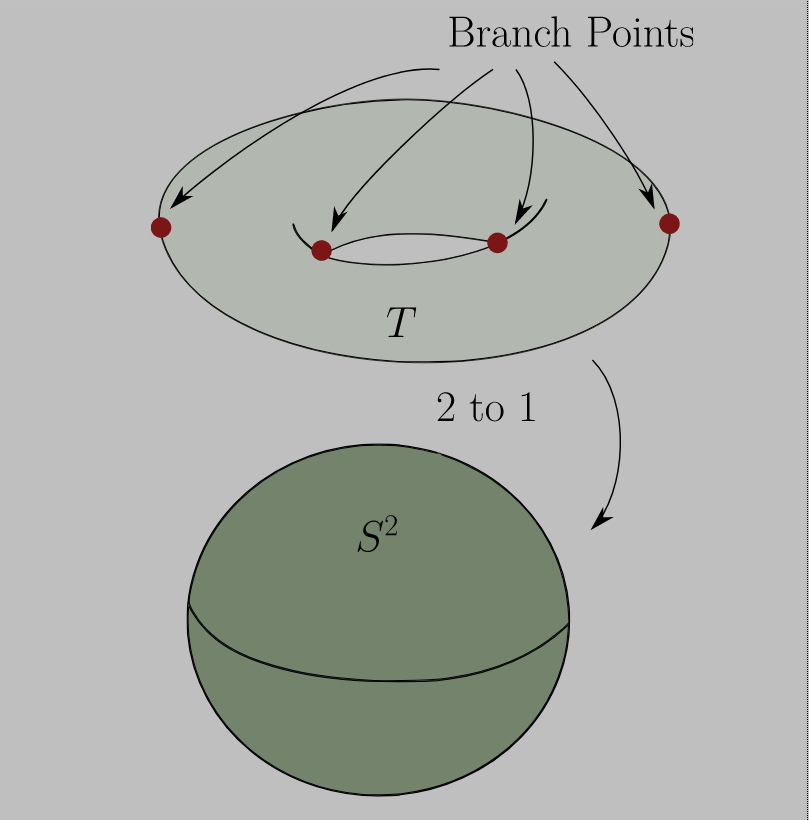
\includegraphics{figures/image_2021-02-25-20-41-53.png}
\caption{image\_2021-02-25-20-41-53}
\end{figure}

Note that homothetic lattices define an isomorphism between the elliptic
curves, and lattices mod homothety are in correspondence of elliptic
curves. By acting
\(\operatorname{PGL}_2(C) \curvearrowright{\mathbb{P}}^1\) since
\(\operatorname{GL}_2\) acts on lines since scaling an element fixes a
line. This is dimension 3. So elliptic curves are also in correspondence
with
\(\left\{{ 4 \text{ points on } {\mathbb{P}}^1}\right\} / \operatorname{PGL}_2({\mathbb{C}})\)
since this is now dimension 1. Note that by applying homothety, the two
basis vectors for a lattice can be rescaled so one is length 1 and the
other is a complex number \(\tau\), and we can identify this space with
\({\operatorname{HH}}/ {\operatorname{SL}}_2({\mathbb{Z}})\).

\end{example}

\begin{exercise}[?]

Show that any \(g(C) = 2\) curve has a degree 2 map to
\({\mathbb{P}}^1\).

\end{exercise}

\begin{remark}

Similarly \(g(C) = 3\) are usually a curve of degree \(4\) in
\({\mathbb{CP}}^2\). Severi proof in the 50s: false! issues with
building moduli space for \(g\geq 23\). Need to use orbifold structure
to take into account automorphisms.

\end{remark}

\hypertarget{wednesday-february-24}{%
\section{Wednesday, February 24}\label{wednesday-february-24}}

Last time:
\begin{align*}
\chi(C, L) 
&= h^0(C, L) - h^1(C, L) \\
&= h^0(C, L) - h^0(C, L ^{-1} \otimes K_C) \\
&= \deg L + 1 -g
,\end{align*}
which is determined by purely topological information. We can generalize
this to arbitrary ranks of the bundle and arbitrary dimensions of
manifold:

\begin{theorem}[Hirzebruch-Riemann-Roch (HRR) Formula]

Let \(X\) be a compact complex manifold and let \(\mathcal{E} \to X\) be
a holomorphic vector bundle. Then
\begin{align*}
\chi( \mathcal{E} ) = \int_C \operatorname{ch}( \mathcal{E} ) \mathrm{td}(X)
.\end{align*}
The constituents here:

\begin{itemize}
\item
  The \textbf{Chern character}, summed over \(R\) the \emph{Chern
  roots}, which is in mixed cohomological degree.
  \begin{align*}
  \operatorname{ch}( \mathcal{E} ) \coloneqq\sum_{x_i \in R} e^{x_i} = \operatorname{ch}_0( \mathcal{E} ) + \operatorname{ch}_1( \mathcal{E} ) + \cdots + \operatorname{ch}_i( \mathcal{E} ) \in H^{2i}(X; {\mathbb{Q}})
  .\end{align*}
\item
  The \textbf{Todd class}, defined as
  \begin{align*}
  \mathrm{td}( F) \coloneqq\prod_{x_i \in R} {x_i \over 1 - e^{-x_i} }
  \end{align*}
  where \(\mathrm{td}(X) \coloneqq\mathrm{td}(TX)\) is viewed as a
  complex vector bundle, which is again in mixed cohomological degree.
\end{itemize}

\end{theorem}

\begin{remark}

Note that integrating over cohomology classes in mixed degree is just
equal to the integral over the top degree terms. Applying this to
\(X = C\) a curve and \(\mathcal{E} \coloneqq{\mathcal{O}}\), we obtain
\begin{align*}
\chi(C, {\mathcal{O}}) 
= \int_C \operatorname{ch}( {\mathcal{O}}) \mathrm{td}(C)
.\end{align*}

We have

\begin{itemize}
\item
  \(\operatorname{ch}({\mathcal{O}}) = e^{c_1({\mathcal{O}})} = e^0 = 1\)
\item
  \(\mathrm{td}(C) \coloneqq\mathrm{td}(TC) = c_1(TC) / (1- e^{ - c_1(TC) } )\),
  whose Taylor coefficients are the Bernoulli numbers. We can expand
  \(x/(1 -e^{-x}) = 1 + (x/2) + (x^2/12) - x^4(720) + \cdots\), and
  since terms above degree 2 vanish, we have
  \begin{align*}
  \cdots 
  &= \int_C 1 + \qty{ 1 + {c_1(TC) \over 2} } \\
  &= \int_C \qty{c_1(TC) \over 2 }\\
  &= {1\over 2} \chi_{\mathsf{Top}}(C) && \text{Chern-Gauss-Bonnet} \\
  &= {2-2g \over 2} \\
  &= 1-g
  .\end{align*}
\end{itemize}

We thus obtain
\begin{align*}
\chi(C, L) 
&= \int_C \operatorname{ch}(L) \mathrm{td}(C) \\
&= \int_C (1 + c_1(L) ) \qty {1 + {c_1(L) \over 2} }\\
&= \int_C c_1(L) + {c_1(TC) \over 2} \\
&= \deg L + 1-g
.\end{align*}

\end{remark}

\begin{remark}

Note that this is a better definition of genus than the previous one,
which was just the correction term in Riemann-Roch. Here we can define
it as \(g \coloneqq h^1/2\).

\end{remark}

\begin{exercise}[?]

Try to state and prove a Riemann-Roch formula for vector bundles on
curves.

\end{exercise}

\begin{proposition}[?]

Let \(S\) be a compact complex surface,
i.e.~\(S\in {\mathsf{Mfd}}_{\mathbb{C}}^2\). An example might be
\(C\times D\) for \(C,D\) two complex curves, or \({\mathbb{CP}}^2\).
Let \(L\to S\) be a holomorphic vector bundle. Then
\begin{align*}
\chi(L) = \chi({\mathcal{O}}_S) + {1\over 2} \qty{ L^2 - L \cdot K}
.\end{align*}
Note that \(L^2 \coloneqq\int_S c_1(L) c_1(L)\) is just shorthand for
taking the intersection of \(L\) with itself. Recall that
\(K \coloneqq\Omega_S^2\) is the space of holomorphic top forms.

\end{proposition}

\begin{proof}[?]

Let \(x_1, x_2\) be the Chern roots of \(TS\). By HRR, we have
\begin{align*}
\chi(L) 
&= \int_S \operatorname{ch}(L) \mathrm{td}(S) \\
&= \int_S \qty{ 1 + c_1(L) + {c_1(L)^2 \over 2!} } \qty{ {x_1 \over 1 - e^{-x_1} } {x_2 \over 1-e^{-x_2}} }\\
&= \int_S \qty{ 1 + c_1(L) + {c_1(L)^2 \over 2!} } \qty{1 + {x_1 \over 2} + {x_1^2 \over 12} }\qty{ 1 + {x_2 \over 2} + {x_2^2\over 12}} \\
&= \int_S \qty{ 1 + c_1(L) + {c_1(L)^2 \over 2!} } \qty{1 + {x_1 + x_2 \over 2} + {x_1^2 + x_2^2 + 3x_1 x_2 \over 12} } \\
&= \int_S \qty{ 1 + c_1(L) + {c_1(L)^2 \over 2!} } \qty{1 + {c_1(x_1, x_2) \over 2} + {c_1(x_1, x_2)^2 + c_2(x_1, x_2) \over 12 } } \\
&= \int_S \qty{ 1 + c_1(L) + {c_1(L)^2 \over 2!} } \qty{1 + { c_1(T) \over 2} + {c_1(T)^2 + c_2(T) \over 2 } } \\
&= \int_S {c_1(L)^2 \over 2} + {c_1(L) c_1(T) \over 2} + {c_1(T)^2 \over 2} + {c_2(T) \over 12} \quad \text{Take deg 4} \\
&= \int_S \qty{ c_1(L)^2 + c_1(L) c_1(T) \over 2} + \chi({\mathcal{O}}_S) \quad \text{HRR on last two terms}
.\end{align*}
where we've applied HRR to \({\mathcal{O}}_S\). It remains to show that
\(c_1(T) = -c_1(K)\). We have
\begin{align*}
K = \Omega_S^2 = \bigwedge\nolimits^2 T^\vee
.\end{align*}
Note that
\(\bigwedge\nolimits^{\text{top}} \mathcal{E} \coloneqq\det( \mathcal{E} )\)
for any bundle \(\mathcal{E}\) since this is a 1-dimensional bundle. We
have \(c_1(T) = -c_1(T^\vee)\) since the Chern roots of \(T^\vee\) are
\(-x_1, -x_2\). So it suffices to show \(c_1(T^\vee) = c_1(K)\), but
there is a general result that
\(c_1(\mathcal{E}) = c_1( \det \mathcal{E} )\). This uses the splitting
principle \(\mathcal{E} = \bigoplus_{i=1}^r L_i\) with
\(x_i = c_1(L_i)\). We have \(c_1(\mathcal{E}) = \sum x_i\) and
\(\det\mathcal{E} = \bigotimes_{i=1}^r L_i\), so
\(\sum x_i = c_1(L_1\otimes\cdots \otimes L_r)\).

\end{proof}

\begin{remark}

We want to use the following formula:
\begin{align*}
\chi(S, L) = \chi({\mathcal{O}}_S) = {1\over 2}(L^2 - L\cdot K)
.\end{align*}
This requires knowing \(\chi({\mathcal{O}}_S)\). Applying HRR yields
\begin{align*}
\chi({\mathcal{O}}_S) 
&= \int_S {c_1(T)^2 + c_2(T) \over 12}\\
&= \int_S { (-c_1(K))^2 + c_2(T) \over 12}\\
&= {K^2 + \displaystyle\int_S c_2(T) \over 12}
,\end{align*}
so we just need to understand \(\int_S c_2(T)\). But for
\(n=\operatorname{rank}\mathcal{E}\), \(c_n( \mathcal{E} )\) (the top
Chern class) is the fundamental class of a zero locus of a section of
\(\mathcal{E}\). Note that \(S \in {\mathsf{Mfd}}_{\mathbb{R}}^4\) is
oriented, so \(\int_S c_2(T)\) is the signed number of zeros of a smooth
vector field.

\begin{figure}
\centering
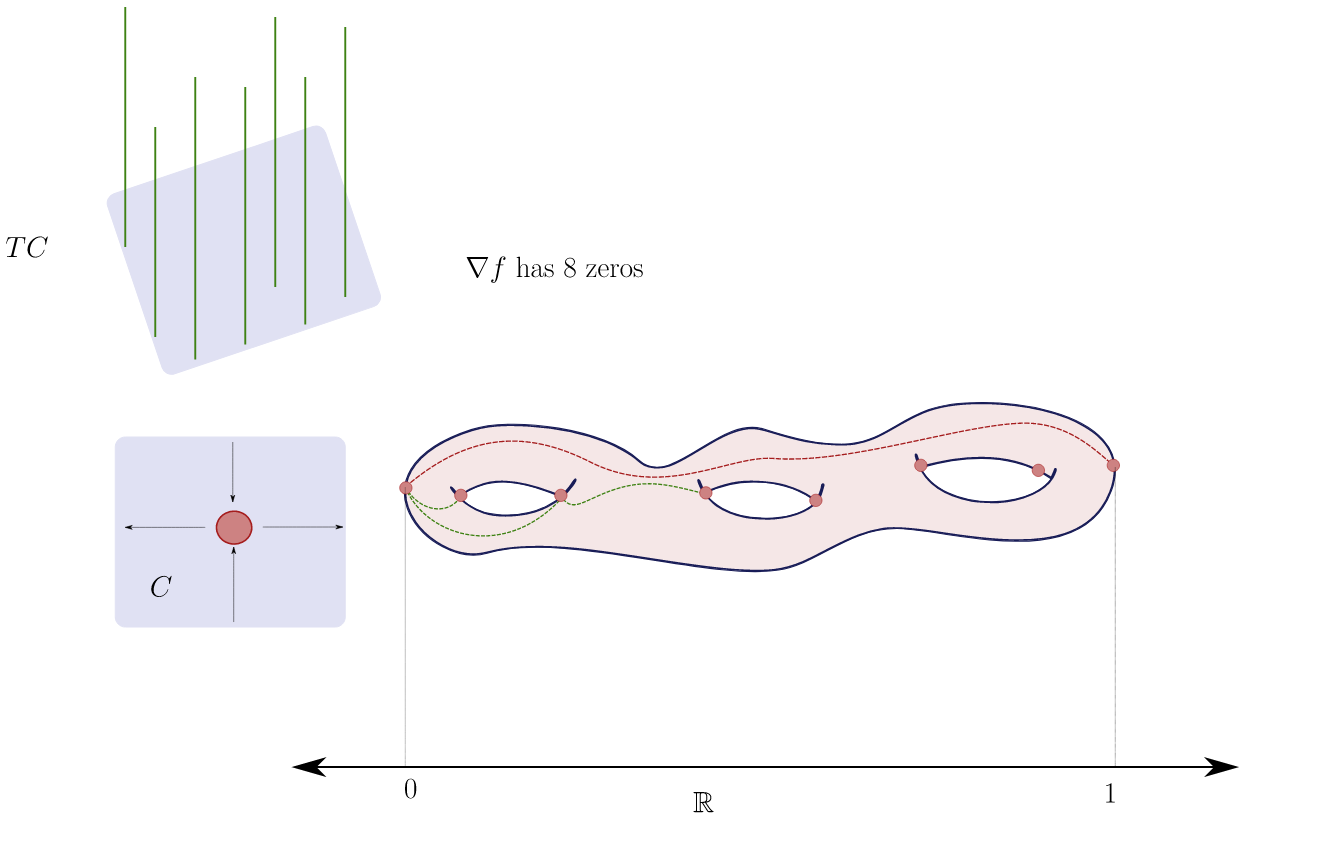
\includegraphics{figures/image_2021-02-25-20-42-49.png}
\caption{image\_2021-02-25-20-42-49}
\end{figure}

Looking at the tangent bundle of the surface, the local sign of an
intersection will be the number of incoming directions \(\pmod 2\),
i.e.~the index of the critical point. Then the signed number of zeros
here yields \(1-6+1 = -4 = \chi_{{\mathsf{Top}}}(C)\). More generally,
we have
\begin{align*}
\chi_{{\mathsf{Top}}}(M^n) = \int_C c_{n}(TM)
,\end{align*}
the \textbf{Chern-Gauss-Bonnet} formula. We can thus write
\begin{align*}
\chi({\mathcal{O}}_S) = {K^2 + \chi_{\mathsf{Top}}(S) \over 12 }
.\end{align*}

\end{remark}

\hypertarget{friday-february-26}{%
\section{Friday, February 26}\label{friday-february-26}}

\begin{remark}

Last time: Riemann-Roch for surfaces, today we'll discuss some examples.
Recall that if \(S \in {\mathsf{Mfd}}_{\mathbb{C}}^2\) is closed and
compact (noting that \(S\in {\mathsf{Mfd}}_{\mathbb{R}}^4\)) and
\(L\to S\) is a holomorphic line bundle then
\begin{align*}
\chi(S, L) = \chi({\mathcal{O}}_S) + {1\over 2}(L^2 - L \cdot K)
\end{align*}
where \(K = c_1(K_S)\) for \(K_S \coloneqq\Omega_S^2\) the canonical
bundle and \(L = c_1(L)\). We also saw
\begin{align*}
\chi({\mathcal{O}}_S) = {1\over 12}(K^2 + \chi_{{\mathsf{Top}}}(S))
,\end{align*}
where \(\chi_{\mathsf{Top}}\) is the Euler characteristic and is given
by
\begin{align*}
\chi_{\mathsf{Top}}(S) = 2 h^0(S; {\mathbb{C}}) - 2 h^1(S, {\mathbb{C}}) + h^2(S; {\mathbb{C}})
.\end{align*}

\end{remark}

\begin{example}[?]

Let \(S = {\mathbb{CP}}^2\), which can be given in local coordinates by
\begin{align*} 
\left\{{ [x_0: x_1: x_2 ] {~\mathrel{\Big|}~}(x_0, x_1, x_2) \in {\mathbb{C}}^3\setminus\left\{{0}\right\}}\right\} 
\end{align*}
where we only take equivalence classes of ratios
\([x,y,z] = [\lambda x, \lambda y, \lambda z]\) for any
\(\lambda\in {\mathbb{C}}^{\times}\). This decomposes as
\begin{align*}
{\mathbb{CP}}^2 \cup{\mathbb{C}}\cup\left\{{ {\{\operatorname{pt}\}}}\right\} = \left\{{ [1: x_1: x_2] }\right\} \cup\left\{{ [0 : x_1: x_2] }\right\} \cup\left\{{ [0:0:1] }\right\}
,\end{align*}
i.e.~we take \(x_0 \neq 0\), then \(x_0 = 0, x_1\neq 0\), then
\(x_0 = x_1 = 0\). Note that
\begin{align*}
h^i({\mathbb{CP}}^n; {\mathbb{Z}}) = 
\begin{cases}
{\mathbb{Z}}&  0 \leq i \leq 2n \text{ even} 
\\
0 & \text{else}.
\end{cases}
\end{align*}

We can use this to conclude that
\(\chi_{\mathsf{Top}}({\mathbb{CP}}^n) = n+1\) and
\(\chi_{\mathsf{Top}}({\mathbb{CP}}^2) = 3\). Over \({\mathbb{CP}}^n\)
we have a \textbf{tautological line bundle} \({\mathcal{O}}(-1)\) given
by sending each point to the corresponding line in
\({\mathbb{C}}^{n+1}\), i.e.~\({\mathcal{O}}(-1) \to {\mathbb{CP}}^n\)
given by
\begin{align*}
\lambda (x_0, \cdots, x_n) \mapsto [x_0: \cdots: x_n]
.\end{align*}
Note that the total space is \(\operatorname{Bl}_0({\mathbb{C}}^{n+1})\)
is the \textbf{blowup} at zero, which separates the tangents at 0.

\end{example}

\begin{remark}

Let \(X\) be an algebraic variety, i.e.~spaces cut out by polynomial
equations, for example
\(\left\{{ xy = 0 }\right\} \subseteq {\mathbb{C}}^2\) which has a
singularity at the origin. A \textbf{divisor} is a
\({\mathbb{Z}}{\hbox{-}}\)linear subvariety of codimension 1. Note that
for a curve \(X\), this gives back the definition in terms of points.
For \(D\) a divisor on \(X\), we associated a bundle
\({\mathcal{O}}_X(D)\) which had a meromorphic section with a zero/pole
locus whose divisor was precisely \(D\).

Recall the construction: we chose a point, then a trivializing
neighborhood where the transition functions where \(V\).

\begin{figure}
\centering
\resizebox{\columnwidth}{!}{%
\begin{tikzpicture}
\fontsize{41pt}{1em} 
\node (node_one) at (0,0) { \import{/home/zack/SparkleShare/github.com/Notes/Class_Notes/2021/Spring/FourManifolds/sections/figures}{2021-02-26_14-12.pdf_tex} };
\end{tikzpicture}
}
\end{figure}

For a higher dimensional algebraic variety or complex manifold, for
\(D\) a complex submanifold, pick a chart around a point that the nearby
portion of \(D\) to a coordinate axis in \({\mathbb{C}}^n\), which
e.g.~can be given by \(\left\{{ z_1 = 0 }\right\}\).

\begin{figure}
\centering
\resizebox{\columnwidth}{!}{%
\begin{tikzpicture}
\fontsize{42pt}{1em} 
\node (node_one) at (0,0) { \import{/home/zack/SparkleShare/github.com/Notes/Class_Notes/2021/Spring/FourManifolds/sections/figures}{2021-02-26_15-58.pdf_tex} };
\end{tikzpicture}
}
\end{figure}

As before there's a distinguished section
\(s_D \in H^0(X; {\mathcal{O}}_X(D) )\) vanishing along \(D\). Note that
a line bundle is a free rank 1 \({\mathcal{O}}{\hbox{-}}\)module, and
analogously here the functions vanishing along \(D\) are
\({\mathcal{O}}{\hbox{-}}\)modules generated by (here) \(z_1\).

\end{remark}

\begin{definition}[Hyperplane]

A \textbf{hyperplane} in \({\mathbb{CP}}^n\) is any set of the form
\begin{align*}
H = \left\{{ [x_0: \cdots : x_1 ] {~\mathrel{\Big|}~}\sum a_i x_i = 0 }\right\} \cong {\mathbb{CP}}^{n-1}
.\end{align*}

\end{definition}

\begin{example}[?]

Take \({\mathbb{CP}}^{n-1} \subseteq {\mathbb{CP}}^n\),
e.g.~\(\left\{{ x_0 = 0 }\right\}\). This is an example of a
\textbf{divisor} on \({\mathbb{CP}}^n\), i.e.~a complex codimension 1
``submanifold''. We can take the line bundle constructed above to get
\({\mathcal{O}}_{{\mathbb{CP}}^n}({\mathbb{CP}}^{n-1})\) which vanishes
along \({\mathbb{CP}}^{n-1}\). More generally, for any hyperplane \(H\)
we can take \({\mathcal{O}}_{{\mathbb{CP}}^n}(H)\), and these are all
isomorphic, so we'll denote them all by
\({\mathcal{O}}_{{\mathbb{CP}}^n}(1)\). The implicit claim is that is
the inverse line bundle of the tautological bundle, so
\({\mathcal{O}}(1) \otimes{\mathcal{O}}(-1)\) is the trivial bundle
since the transition functions are given by reciprocals and multiplying
them yields 1. We can classify complex line bundles on
\({\mathbb{CP}}^n\) using the SES
\begin{align*}
0 \to \underline{{\mathbb{Z}}} \to {\mathcal{O}}\xrightarrow{\exp} {\mathcal{O}}^{\times}\to 1
.\end{align*}

We know that \(H^1(X; {\mathcal{O}}^{\times})\) were precisely
holomorphic line bundles, since they were functions agreeing on double
overlaps with a cocycle condition. We have a LES coming from sheaf
cohomology:

\begin{center}
\begin{tikzcd}
    &&&& \cdots \\
    \\
    {H^1(X; {\mathcal{O}})} && {H^1(X; {\mathcal{O}})} && {H^1(X; {\mathcal{O}}^{\times})} \\
    \\
    {H^2(X; {\mathcal{O}})} && \cdots
    \arrow["{c_1}", from=3-5, to=5-1, out=0, in=180]
    \arrow[from=3-1, to=3-3]
    \arrow[from=3-3, to=3-5]
    \arrow[from=5-1, to=5-3]
    \arrow[from=1-5, to=3-1, out=0, in=180]
\end{tikzcd}
\end{center}

\begin{quote}
\href{https://q.uiver.app/?q=WzAsNixbMiwyLCJIXjEoWDsgXFxPTykiXSxbNCwyLCJIXjEoWDsgXFxPT1xcdW5pdHMpIl0sWzAsNCwiSF4yKFg7IFxcT08pIl0sWzAsMiwiSF4xKFg7IFxcT08pIl0sWzQsMCwiXFxjZG90cyJdLFsyLDQsIlxcY2RvdHMiXSxbMSwyLCJjXzEiXSxbMywwXSxbMCwxXSxbMiw1XSxbNCwzXV0=}{Link
to Diagram}
\end{quote}

Applying this to \(X\coloneqq{\mathbb{CP}}^n\), we have
\(H^1({\mathcal{O}}) = H^2({\mathcal{O}}) = 0\). This can be computed
directly using that \({\mathbb{CP}}^n = \cup_{n\geq 1} {\mathbb{C}}^n\)
by taking charts \(x_i\neq 0\), and this yields an acyclic cover. Thus
\(c_1\) is an isomorphism above, and
\({\operatorname{Pic}}({\mathbb{CP}}^n) \cong {\mathbb{Z}}\), where
\({\operatorname{Pic}}\) denotes isomorphism classes of line bundles. We
can identify
\({\operatorname{Pic}}({\mathbb{CP}}^n) = \left\{{ {\mathcal{O}}_{{\mathbb{CP}}^n}(k) {~\mathrel{\Big|}~}k\in {\mathbb{Z}}}\right\}\).

\end{example}

\hypertarget{monday-march-01}{%
\section{Monday, March 01}\label{monday-march-01}}

\begin{remark}

Last time: we defined \({\operatorname{Pic}}({\mathbb{CP}}^n)\) as the
set of line bundles on \({\mathbb{CP}}^n\).

\end{remark}

\begin{definition}[Picard Group of a Manifold]

Given any \(X\in {\mathsf{Mfd}}_{\mathbb{C}}\), define
\({\operatorname{Pic}}(X)\) as the set of isomorphism classes of
holomorphic line bundles on \(X\). This is an abelian group given by
\(L \otimes L'\) and inversion \(L\to L^{-1}\).

\end{definition}

\begin{remark}

We saw that
\({\operatorname{Pic}}(X) \cong H^1(X; {\mathcal{O}}^{\times})\) as
groups, noting that \(H^1\) has a natural group structure here. We
defined a \textbf{tautological bundle} on \({\mathbb{CP}}^n\) and saw it
was isomorphic to \({\mathcal{O}}(-1)\), and moreover
\({\mathcal{O}}(H) \cong {\mathcal{O}}(1)\) for \(H\) a hyperplane. The
fiber was given by
\begin{align*}
\mathrm{Taut} &\to {\mathbb{CP}}^n \\
\left\{{ \lambda (x_0, \cdots, x_n) {~\mathrel{\Big|}~}\lambda\in {\mathbb{C}}}\right\} &\mapsto [x_0: \cdots : x_n]
,\end{align*}
i.e.~the entire line corresponding to the given projective point. We
also have \({\mathcal{O}}(H)(U)\) is the sect of rational homogeneous
functions \(\phi\) on \(U\) of degree 1 such that
\(\operatorname{Div}\phi + H \geq 0\) where
\(H \coloneqq\left\{{x_0 = 0}\right\}\). We want \(\phi/x_0\) to be a
well-defined function, so \(\phi\) should scale like \(x_0\) in the
sense that
\begin{align*}
\phi( \lambda x_0, \cdots, \lambda x_n) = \lambda\phi( x_0, \cdots, x_n)
.\end{align*}
Note that there is a natural map
\begin{align*}
{\operatorname{Taut}}\otimes{\mathcal{O}}(H) \xrightarrow{} {\mathcal{O}}
,\end{align*}
given by taking the line over a point and evaluating the homogeneous
function on that line. Thus \({\operatorname{Taut}}\) is the inverse of
\({\mathcal{O}}(H)\).

\end{remark}

\begin{remark}

We want to understand what Noether's formula says for
\({\mathbb{CP}}^2\), which requires understanding the canonical bundle
\(K_{{\mathbb{CP}}^n}\). We'll do this by writing down a meromorphic
section \(\omega\) (since it's a meromorphic volume form) which will
yield \(K_{{\mathbb{CP}}^n} = {\mathcal{O}}(\operatorname{Div}\omega)\).
So take
\begin{align*}
\omega \coloneqq x_1^{-1}dx_1 \wedge \cdots \wedge x_n^{-1}dx_n 
,\end{align*}
noting that we leave out the first coordinate \(x_0\) and divide by
coordinates to make this scale-invariant. Here we work in a
\({\mathbb{C}}^n\) chart of points of the form
\([1: x_1 : \cdots : x_n]\). Where does \(\omega\) have poles? Along
\(x_i = 0\) for any \(1\leq i \leq n\), and similarly in any other
coordinate chart. We also have a 1st order pole along \(x_0 = 0\). We
then get
\begin{align*}
K_{{\mathbb{CP}}^n} = {\mathcal{O}}(\operatorname{Div}\omega) = {\mathcal{O}}( -H_0 -H_1 - \cdots - H_n) = {\mathcal{O}}(-n-1)
,\end{align*}
where \(H_i = \left\{{x_i = 0}\right\}\).

Note that \({\mathbb{CP}}^n\) is like a simplex:

\begin{figure}
\centering
\resizebox{\columnwidth}{!}{%
\begin{tikzpicture}
\fontsize{45pt}{1em} 
\node (node_one) at (0,0) { \import{/home/zack/SparkleShare/github.com/Notes/Class_Notes/2021/Spring/FourManifolds/sections/figures}{2021-03-01_14-12.pdf_tex} };
\end{tikzpicture}
}
\end{figure}

Applying this to \({\mathbb{CP}}^2\), we obtain
\begin{align*}
K_{{\mathbb{CP}}^2} = {\mathcal{O}}(-3)
.\end{align*}
What is the intersection form? We know
\(H^2({\mathbb{CP}}^2; {\mathbb{Z}}) \cong {\mathbb{Z}}\) and the
intersection form is unimodular. So write
\({\mathbb{Z}}\coloneqq{\mathbb{Z}}\alpha\) for \(\alpha\) some
generator. Then \(\alpha \cdot \alpha = \pm 1\) since \(\det G = \pm 1\)
for the Gram matrix for this to be unimodular. Note that
\((- \alpha) \cdot (- \alpha) = \pm 1\) with the same sign.

\begin{claim}

\({\mathcal{O}}(1) = {\mathcal{O}}(H)\) generates
\({\operatorname{Pic}}({\mathbb{CP}}^2) = H^2({\mathbb{CP}}^2; {\mathbb{Z}})\).

\end{claim}

This is because
\(c_1 {\mathcal{O}}(H) \cdot c_1 {\mathcal{O}}(H) = H\cdot H = \left\{{ x_0 = 0 }\right\} \pitchfork\left\{{ x_1 = 0 }\right\} = \left\{{ [0:0:1] }\right\}\)
here we note that the two hyperplanes can be oriented transversely and
intersected. This is an oriented intersection.

Recall Noether's formula, which was HRR applied to \({\mathcal{O}}\) and
the Chern-Gauss-Bonet theorem:
\begin{align*}
\chi({\mathcal{O}}) 
&= {1\over 12}(K^2 + \chi_{\mathsf{Top}})\\
&= h^0({\mathcal{O}}) - h^1({\mathcal{O}}) + h^2({\mathcal{O}})\\
&= 1 -1 + 1\\
&= 1
.\end{align*}
The right-hand side can be written as
\begin{align*}
{1\over 12} \qty{ (-3H) \cdot (-3H) + 3} = {1\over 12}(9+3) = 1
.\end{align*}

\end{remark}

\begin{proposition}[?]

\(S^4\) has no complex structure.

\end{proposition}

\begin{proof}[?]

We know that \(\chi_{\mathsf{Top}}(S^4) = 2\). If \(S^4\) had a complex
structure, then \(c_1(K_{S^4}) \in H^2(S^4; {\mathbb{Z}}) = 0\). Thus
would make \(K_{S^4}^2 = 0\), and so
\begin{align*}
\chi( {\mathcal{O}}_{S^4} ) = {1\over 12}( 0 + 2) = {1\over 6} \not\in {\mathbb{Z}}
,\end{align*}

which is a contradiction. \(\contradiction\)

\end{proof}

\begin{example}[?]

Consider
\(\mkern 1.5mu\overline{\mkern-1.5mu{\mathbb{CP}}\mkern-1.5mu}\mkern 1.5mu^2\),
a 4-manifold diffeomorphic to \({\mathbb{CP}}^2\) with the opposite
orientation. What is the intersection form? Taking \(H\cdot H = -1\)
since the orientations aren't compatible, and more generally the Gram
matrix is negated when the orientation is reversed.

\end{example}

\begin{proposition}[?]

\(\mkern 1.5mu\overline{\mkern-1.5mu{\mathbb{CP}}\mkern-1.5mu}\mkern 1.5mu^2\)
is not diffeomorphic to a complex surface by an orientation-preserving
diffeomorphism (or any homeomorphism).

\end{proposition}

\begin{proof}[?]

We have \(\chi_{\mathsf{Top}}= 3\), and
\(K_{\mkern 1.5mu\overline{\mkern-1.5mu{\mathbb{CP}}\mkern-1.5mu}\mkern 1.5mu^2} = -c_1(T \mkern 1.5mu\overline{\mkern-1.5mu{\mathbb{CP}}\mkern-1.5mu}\mkern 1.5mu^2) = \pm 3H\).
Then
\begin{align*}
\chi({\mathcal{O}}) = {1\over 12}\qty{ K_{\mkern 1.5mu\overline{\mkern-1.5mu{\mathbb{CP}}\mkern-1.5mu}\mkern 1.5mu^2}^2 + \chi_{\mathsf{Top}}} = {1\over 12}(-9+3) \not\in {\mathbb{Z}}
.\end{align*}

\end{proof}

\begin{remark}

Consider \({\mathcal{O}}_{{\mathbb{CP}}^n}(d)\), what are its global
sections \(H^0({\mathbb{CP}}^n, {\mathcal{O}}_{{\mathbb{CP}}^n}(d))\).
Locally we have \({\mathcal{O}}_{{\mathbb{CP}}^n}(d)(U)\) given by
holomorphic functions in \((x_0, \cdots, x_n) \in \pi^{-1}(U)\) where
\(\pi: {\mathbb{C}}^{n+1} \to {\mathbb{CP}}^n\) and the functions
satisfy \(f(\lambda \mathbf{x}) = \lambda^d f(\mathbf{x})\). The global
sections will be the homogeneous degree \(d\) polynomials in the
coordinates of \(\mathbf{x}\).

\end{remark}

\begin{remark}

Why does a holomorphic function
\(f: {\mathbb{C}}^{n+1} \to {\mathbb{C}}\) such that
\(f(\lambda \mathbf{x}) = \lambda^d f(\mathbf{x})\) necessarily a
polynomial? Use the result that any such function with at most
polynomial growth is itself a polynomial. If
\({ \left.{{f}} \right|_{{S^{2d+1}}} }\) is bounded by \(C\), we have
\({\left\lVert {f} \right\rVert}_{L^2} \leq C {\left\lvert {x} \right\rvert}^{2d}\).
Since \(({{\partial}}_{x_1} \cdots {{\partial}}_{x_k})^d f\) is globally
bounded \(k\geq 2d\), applying Liouville's theorem makes it constant,
and so a finite number of derivatives kill \(f\) and this forces it to
be polynomial.

\end{remark}

\begin{remark}

So how many homogeneous degree \(d\) functions are there? Here
\(h^0({\mathbb{CP}}^n, {\mathcal{O}}(d)) =\) will be the number of
linearly independent degree \(d\) polynomials in the variables
\(x_0, \cdots, x_n\), which is
\({\left(\kern-.3em\left(\genfrac{}{}{0pt}{}{n+1}{d}\right)\kern-.3em\right)} = {n + d\choose n}\),
using the fact that monomials span this space.

\end{remark}

\begin{exercise}[?]

Using that
\(h^0({\mathbb{CP}}^2; {\mathcal{O}}(k))= h^2({\mathbb{CP}}^2; {\mathcal{O}}(-3-k) )\)
by Serre duality and Riemann-Roch, compute
\(h^i({\mathbb{CP}}^2; {\mathcal{O}}(k))\) for all \(i, k\).

\end{exercise}

\begin{fact}

\(h^i({\mathbb{CP}}^n; {\mathcal{O}}(k)) = 0\) unless \(i=0, n\).

\end{fact}

\hypertarget{wednesday-march-03}{%
\section{Wednesday, March 03}\label{wednesday-march-03}}

Find first 5m.

\begin{remark}

When we considered
\(\mkern 1.5mu\overline{\mkern-1.5mu{\mathbb{CP}}\mkern-1.5mu}\mkern 1.5mu^2\),
we implicitly assumed
\(T\mkern 1.5mu\overline{\mkern-1.5mu{\mathbb{CP}}\mkern-1.5mu}\mkern 1.5mu^2\)
was a complex rank 2 vector bundle with some purported complex
structure.

\end{remark}

\begin{claim}

\begin{align*}
c_1( T\mkern 1.5mu\overline{\mkern-1.5mu{\mathbb{CP}}\mkern-1.5mu}\mkern 1.5mu^2) = \pm 3H
,\end{align*}
although it's not clear that
\(c_1(K) \in H^2( \mkern 1.5mu\overline{\mkern-1.5mu{\mathbb{CP}}\mkern-1.5mu}\mkern 1.5mu^2; {\mathbb{Z}}) \cong ({\mathbb{Z}}, [-1] )\).

\end{claim}

\begin{remark}

We had
\(\chi({\mathcal{O}}) = {1\over 12} \qty{ K^2 + \chi_{\mathsf{Top}}} = {1\over 12}(3-n^2)\),
and since \(3-n^2 \in 12{\mathbb{Z}}\), we have
\(n^2 \in 3 + 12{\mathbb{Z}}\subset 3 + 4{\mathbb{Z}}\) and this forces
\(n^2 \equiv 3 \pmod 4\).

\end{remark}

\begin{definition}[Differential Complex]

Let
\begin{align*}
0 \to \mathcal{E}^0 \xrightarrow{d_0} \mathcal{E}^1 \xrightarrow{d_1} \cdots \to \mathcal{E}^n \to 0
\end{align*}
be a complex (so \(d^2 = 0\)) of smooth vector bundles on a smooth
manifold \(X\operatorname{im}{\mathsf{Mfd}}_{\mathbb{R}}^{C^\infty}\).
Suppose that the \(d_i\) are \textbf{differential operators}, i.e.~in
local trivializing charts over \(U\) we have

\begin{align*}
\mathcal{E}^i \cong {\mathcal{O}}^{\oplus r_i} {\mathcal{O}}^{\oplus r_{i+1}} \cong \mathcal{E}^{i+1}
\end{align*}
where in every matrix coordinate, \(d_i\) is of the form
\(\sum_{{\left\lvert {I} \right\rvert} < N} g_I {{\partial}}_I\) where
\({{\partial}}_I \coloneqq{{\partial}}_{i_1} \cdots {{\partial}}_{i_N}\)
is a partial derived and the \(g_I\) are smooth functions.

\end{definition}

\begin{example}[?]

For \(X\in {\mathsf{Mfd}}_{\mathbb{R}}^{C^ \infty }\), we can take
\begin{align*}
0 \to {\mathcal{O}}\xrightarrow{d} \Omega^1 \xrightarrow{d} \Omega^2 \xrightarrow{d} \cdots
.\end{align*}
In local coordinates,

\begin{itemize}
\tightlist
\item
  \(\Omega^1\) is spanned over \({\mathcal{O}}\) by
  \(dx_1, \cdots, dx_n\) where \(n = \dim_{\mathbb{R}}(X)\)
\item
  \(\Omega^2\) is spanned over \({\mathcal{O}}\) by \(dx_i \wedge dx_j\)
  for \(1\leq i, j \leq n\).
\end{itemize}

Then the component of \(d\) sending \(dx_i \to dx_i \wedge dx_j\) is of
the form
\begin{align*}
fdx_i &\mapsto -{\frac{\partial f}{\partial x_j}\,} dx_i \wedge dx_j
.\end{align*}

\end{example}

\begin{example}[?]

For \(X\in {\mathsf{Mfd}}_{\mathbb{C}}\) and \(\mathcal{E} \to X\) a
holomorphic vector bundle, take
\begin{align*}
\mathcal{E} \otimes A^{0,0} \xrightarrow{\mkern 1.5mu\overline{\mkern-1.5mu{\partial}\mkern-1.5mu}\mkern 1.5mu} \mathcal{E} \otimes A^{0, 1} \xrightarrow{\mkern 1.5mu\overline{\mkern-1.5mu{\partial}\mkern-1.5mu}\mkern 1.5mu} \mathcal{E} \otimes A^{0, 2} \to \cdots
.\end{align*}
This is because for \(s_i\) local holomorphic sections and \(\omega\) a
smooth form we have
\begin{align*}
\mkern 1.5mu\overline{\mkern-1.5mu{\partial}\mkern-1.5mu}\mkern 1.5mu\qty{ (s_1, \cdots, s_r) \otimes\omega } = \qty{s_1, \cdots, s_r} \otimes\mkern 1.5mu\overline{\mkern-1.5mu{\partial}\mkern-1.5mu}\mkern 1.5mu\omega
.\end{align*}

\end{example}

\begin{definition}[Order of an operator]

The maximal \(N\) that appears in
\(\sum_{ {\left\lvert {I} \right\rvert} \leq N} g_I {{\partial}}_I\) is
the \textbf{order}.

\end{definition}

\begin{definition}[Symbol Complex]

The \textbf{symbol complex} is a sequence of vector bundles on
\(T^\vee X\). Noting that we have \(\pi: T^\vee X\to X\), and using
pullbacks we can obtain bundles over the cotangent bundle:
\begin{align*}
0 \to \pi^* \mathcal{E}_0 \xrightarrow{\sigma(d_0)} \pi^* \mathcal{E}_1 \xrightarrow{\sigma(d_1)} \cdots \to \pi^* \mathcal{E}_n \to 0
.\end{align*}
The \textbf{symbol} of the differential operator \(d_i\) is
\(\sigma(d_i)\). It is defined by replacing \({\partial}_i\) in
\(\sum_{{\left\lvert {I} \right\rvert} {\color{red} =} N } g_I {\partial}_I\)
with \(y_i\) where
\begin{align*}
y_i: T^\vee U \to {\mathbb{R}}
\end{align*}
is the coordinate function on the second factor of
\(T^\vee U = U \times{\mathbb{R}}^n\) associated to the local coordinate
\(i\). Using that \(TU = (T^\vee)^\vee U\), we can view \({\partial}_i\)
as functions on the cotangent bundle, \(\sigma(d_i)\) is given in local
trivializations by multiplication by a smooth function
\(\sum_{{\left\lvert {I} \right\rvert} = N} g_I y^I\).

\end{definition}

\begin{example}[?]

Consider \({\mathcal{O}}\xrightarrow{d} \Omega^1\). In local
coordinates, this is given by
\(d = \qty{{\partial}_1, \cdots, {\partial}_n}\), i.e.~coordinate-wise
differentiation, since we can write a local trivialization
\(\Omega^1 = {\mathcal{O}}dz_1 \oplus \cdots \oplus {\mathcal{O}}dz_n\).
Then the symbol of \(d\) is given by
\begin{align*}
\sigma(d): \pi^* {\mathcal{O}}&\to \pi^* \Omega^1 \\
1 &\mapsto (y_1, \cdots, y_n) 
,\end{align*}
thought of as vector bundles over \(T^\vee X\), and this is projection
onto to cotangent factor. Locally, the image of 1 is given by
\(y_1 dx_1 + \cdots y_n dx_n\), which is a point in \(T_p^\vee X\) for
all \((p, \alpha) \in T^\vee X\) which is an assignment to every point
\((p, \alpha) \in T_p^\vee X\) a point in
\((\pi^* \Omega^1)_{p, \alpha} \cong T_p^\vee X\). There is a
tautological section
\((p, \alpha) \to \alpha\in T_p^\vee X\in (\pi^* \Omega^1)_{p, \alpha}\),
or really \((p, \alpha) \mapsto ( (p, \alpha), \alpha)\).

\end{example}

\begin{remark}

See similarly to the canonical symplectic structure of the cotangent
bundle.

\end{remark}

\begin{remark}

More generally, for \(d: \Omega^p \to \Omega^{p+1}\), \(\sigma(d)\) acts
on the frame \(dx_{i_1} \wedge \cdots dx_{i_p}\) in the following way:
\begin{align*}
\sigma(d)(dx_{i_1} \wedge \cdots \wedge dx_{i_p}) = \sum_y y_y dx_j \wedge dx_{i_1} \wedge \cdots dx_{i_p}
\end{align*}
where
\begin{align*}
d: fdx_{i_1} \wedge \cdots \wedge dx_{i_p} \mapsto \sum_j {\frac{\partial f}{\partial x_j}\,} dx_j \wedge \qty{dx_{i_1} \wedge \cdots \wedge dx_{i_p}}
.\end{align*}
The symbol complex is
\begin{align*}
\pi^* {\mathcal{O}}\xrightarrow{\sigma(d)} \pi^* \Omega^1 \xrightarrow{\sigma(d)} \pi^* \Omega^2 \to \cdots \to \pi^* \Omega^n \to 0
\end{align*}
for \(n\) the dimension. In this case, \(\sigma(d)\) has the same
formula everywhere, since it's \(C^ \infty {\hbox{-}}\)linear:
\begin{align*}
\sigma(d) = \sum_j y_j dx_j \wedge \qty{\cdots}
.\end{align*}

\end{remark}

\begin{definition}[Elliptic Complex]

A differential complex \(({\mathcal{E}}^{{\,\cdot\,}}, d)\) is
\textbf{elliptic} if the symbol complex
\((\pi^* {\mathcal{E}}^{{\,\cdot\,}}, \sigma(d))\) is an exact sequence
of sheaves (importantly) on \(T^\vee X \setminus\left\{{s_z}\right\}\)
for \(s_z\) the zero section.

\end{definition}

\begin{claim}

\(({\Omega}^{{\,\cdot\,}}, d)\) is elliptic. To check exactness of a
sequence of vector bundles, it suffices to check exactness on every
fiber. Fix \((p, \alpha) \in T^\vee X \setminus\left\{{ s_z }\right\}\),
then
\begin{align*}
0 \to {\mathbb{C}}\xrightarrow{\wedge \alpha}  T^\vee_p X \xrightarrow{\wedge \alpha}  \bigwedge^2 T_p^\vee X \xrightarrow{\wedge \alpha}  \bigwedge^3 T_p^\vee X \to \cdots
.\end{align*}
Moreover, if \(\alpha\wedge \beta = 0\) implies that
\(\beta = \alpha\wedge \gamma\) for some \(\gamma\), which implies that
this sequence is exact.

\end{claim}

\hypertarget{friday-march-05}{%
\section{Friday, March 05}\label{friday-march-05}}

\begin{remark}

Recall that we set up a differential complex, whose objects were vector
bundles and differentials were differential operators (i.e.~linear
combinations of partial derivatives) in local trivializations. We pulled
back to tangent bundles (?) and defined the \emph{symbol} of an
operator, and saw that when taking the symbol complex of the deRham
complex. the sequence of maps was given by wedging against a
tautological one-form. This was an \emph{elliptic complex} because the
maps became wedging with a covector.

\end{remark}

\begin{example}[of an elliptic complex]

Let \(X\in {\mathsf{Mfd}}_{\mathbb{C}}\) and
\(\mathcal{E}\to X \in {\mathsf{VectBundle}}_{\mathbb{C}}\) be
holomorphic. There is a resolution
\begin{align*}
0 \to \mathcal{E} \xrightarrow{i} \mathcal{E} \otimes A^{0, 0} \xrightarrow{\mkern 1.5mu\overline{\mkern-1.5mu{\partial}\mkern-1.5mu}\mkern 1.5mu} \mathcal{E} \otimes A^{0, 1} \xrightarrow{\mkern 1.5mu\overline{\mkern-1.5mu{\partial}\mkern-1.5mu}\mkern 1.5mu} \cdots
.\end{align*}
What is the symbol complex? Consider the projection
\(\pi: T^\vee X\to X\), and use pullbacks to get a sequence
\begin{align*}
0 \to \pi^* \mathcal{E} \otimes A^{0, 0} \xrightarrow{\sigma( \mkern 1.5mu\overline{\mkern-1.5mu{\partial}\mkern-1.5mu}\mkern 1.5mu)} \pi^* \mathcal{E} \otimes A^{0, 1} \xrightarrow{\sigma( \mkern 1.5mu\overline{\mkern-1.5mu{\partial}\mkern-1.5mu}\mkern 1.5mu)} \cdots
.\end{align*}
Here the symbol
\(\sigma(\mkern 1.5mu\overline{\mkern-1.5mu{\partial}\mkern-1.5mu}\mkern 1.5mu)\)
replace \({\frac{\partial }{\partial t {\overline{{z}}}_i}\,}\) with the
corresponding function on \(T^\vee X\), say \({\overline{{y}}}_i\). Then
\(\sigma( \mkern 1.5mu\overline{\mkern-1.5mu{\partial}\mkern-1.5mu}\mkern 1.5mu) = \sum_i {\overline{{y}}}_i \, d{\overline{{z}}}_i \wedge ({\,\cdot\,}) = {\overline{{ \alpha }}} \wedge ({\,\cdot\,})\).
As before, at a point \((p, \alpha)\) where \(\alpha\neq 0\) in
\(T^\vee X\), we get
\begin{align*}
0 \to \mathcal{E}_p \xrightarrow{{\overline{{ \alpha}}} \wedge ({\,\cdot\,})} \mathcal{E}_p \otimes\bigwedge^{0, 1}_p X \xrightarrow{{\overline{{ \alpha }}} \wedge ({\,\cdot\,})} \mathcal{E}_p \otimes\bigwedge^{0, 2} X \to \cdots
,\end{align*}
which is an exact sequence of vector spaces. So
\(( \mathcal{E} \otimes A^{0, p}, \mkern 1.5mu\overline{\mkern-1.5mu{\partial}\mkern-1.5mu}\mkern 1.5mu)\)
is an elliptic complex.

\end{example}

\begin{slogan}

The symbol being exact is approximately the top-order part being
nowhere-vanishing.

\end{slogan}

\begin{remark}

The next theorem computes the cohomology of an elliptic complex using
Chern and Todd classes.

\end{remark}

\begin{theorem}[Atiyah-Singer Index Theorem]

If \(( {\mathcal{E}}^{{\,\cdot\,}}, d)\) is an elliptic complex of
smooth vector bundles on a compact oriented
\(X\in {\mathsf{Mfd}}^n_{\mathbb{R}}\), then
\begin{align*}
\chi({ \mathcal{E} }^{{\,\cdot\,}}, d) = \sum (-1)^i \dim \qty{\ker d^i \over \operatorname{im}d^{i-1} } = 
(-1)^{\dim(X) \choose 2}
\int_X {\operatorname{ch}\over {\operatorname{eul}}}( {\mathcal{E}}^{{\,\cdot\,}} ) \mathrm{td}(TX \otimes_{\mathbb{R}}{\mathbb{C}})
.\end{align*}

\end{theorem}

\begin{remark}

Here we define
\(\operatorname{ch}( {\mathcal{E}}^{{\,\cdot\,}} \coloneqq\sum_i (-1)^i \operatorname{ch}( \mathcal{E}^i )\).
What does it mean to divide by the Euler class? Let
\(\left\{{ x_i, -x_i }\right\}\) be the Chern roots of the complexified
tangent bundle \(TX\otimes{\mathbb{C}}\), then
\({\operatorname{eul}}(X) \coloneqq\prod x_i\) is the product where we
pick one of each of the Chern roots from each of the pairs. The
preferred sign to choose is the one for which
\(\int_X \prod x_i = \chi_{\mathsf{Top}}(X)\). Dividing just means to
take the Chern character, then if it's divisible by \(\prod x_i\), we do
so. We have
\begin{align*}
\mathrm{td}(TX\otimes{\mathbb{C}}) = \prod_i 
\qty{x_i \over 1 - e^{-x_i}} 
\qty{-x_i \over 1 - e^{-x_i}} 
.\end{align*}

Thus
\begin{align*}
{\mathrm{td}(TX\otimes{\mathbb{C}}) \over {\operatorname{eul}}(X) } = 
\prod_i {1\over x_i}
\qty{x_i \over 1 - e^{-x_i}} 
\qty{-x_i \over 1 - e^{-x_i}} 
,\end{align*}
but note that this doesn't necessarily make sense. However, all all
computations we'll see, there will be enough cancellation to make this
well-defined.

\end{remark}

\begin{exercise}[Chern character of the de Rham complex]

\(\operatorname{ch}( {\Omega}^{{\,\cdot\,}}X \otimes{\mathbb{C}}) = \prod_i (1-e^{x_i}) (1 - e^{-x_i})\)
for \(X\in {\mathsf{Mfd}}_{\mathbb{R}}^{2n}\) even dimensional.

\end{exercise}

\begin{example}[?]

Supposing \(X\in {\mathsf{Mfd}}_{\mathbb{R}}^2\) is a genus \(g\)
surface, we have
\begin{align*}
{\mathcal{O}}\to \Omega^1\otimes{\mathbb{C}}\to \Omega^2 \otimes{\mathbb{C}}
,\end{align*}
and
\(\operatorname{ch}({ \Omega }^{{\,\cdot\,}}) = \operatorname{ch}( {\mathcal{O}}) - \operatorname{ch}( \Omega^1 \otimes{\mathbb{C}}) + \operatorname{ch}(\Omega^2\otimes{\mathbb{C}})\).
The Chern roots of \(TX \otimes{\mathbb{C}}\) are
\(\left\{{ x_i, -x_i }\right\}\), which come in pairs. So
\begin{align*}
\operatorname{ch}( {\Omega}^{{\,\cdot\,}} ) 
= 1 - e^{x_i} - e^{x_i} + e^{-x_i + x_i}
= (1 - e^{-x_i})( 1 - e^{x_i} )
.\end{align*}
From the theorem, we're supposed to have
\begin{align*}
\chi( {\Omega}^{{\,\cdot\,}}, d) 
&= 
(-1)^{n(n-1) \over 2}
\int_X
{\prod_i (1 - e^{-x_i})( 1 - e^{x_i} ) \over \prod_{i=1}^n x_i }
\prod_i 
\qty{x_i \over 1 - e^{-x_i}} 
\qty{-x_i \over 1 - e^{-x_i}} \\
&= 
(-1)^{n(n-1) \over 2}
\int_X
\prod_{i=1}^n (-x_i)\\
& = \int_X 
\prod_i x_i \\
&=
\chi_{\mathsf{Top}}(X) && \text{C-G-B}
.\end{align*}
Letting \(d=\dim X = 2n\), we have
\begin{align*}
(-1)^n (-1)^{d(d-1) \over 2} = (-1)^n (-1)^{n(2n-1)} = (-1)^2n = 1 .
\end{align*}

\end{example}

\begin{example}[?]

We have prove HRR using this theorem: we have
\begin{align*}
\chi(X, \mathcal{E} ) = \chi( \mathcal{E} \otimes A^{0, {\,\cdot\,}}, \mkern 1.5mu\overline{\mkern-1.5mu{\partial}\mkern-1.5mu}\mkern 1.5mu) \overset{\text{ASIT}}{=} \int_X { \operatorname{ch}(\mathcal{E} \otimes A^{0, {\,\cdot\,}} ) \over {\operatorname{eul}}(X) } \mathrm{td}(TX \otimes_R {\mathbb{C}})
.\end{align*}
We have
\(\operatorname{ch}( \mathcal{E} \otimes A^{0, {\,\cdot\,}} ) = \operatorname{ch}(\mathcal{E}) \operatorname{ch}( A^{0, {\,\cdot\,}} )\)
where
\(\operatorname{ch}(A^{0, 1}) = \sum_I (-1)^i \operatorname{ch}(\bigwedge^i A^{0, 1} )\).
The Chern roots of

\begin{itemize}
\tightlist
\item
  \(TX\) are \(\left\{{ x_i }\right\}\)\\
\item
  \(A^{1, 0} = T^\vee X\) are \(\left\{{ -x_i }\right\}\)\\
\item
  \(A^{0, 1}\) are \(\left\{{ -x_i }\right\}\)
\end{itemize}

So we obtain
\begin{align*}
\chi( \mathcal{E} ) 
&= (-1)^n \int_X {\prod ( 1- e^{x_i}) \over \prod x_i}
\prod_i 
\qty{x_i \over 1 - e^{-x_i}} 
\qty{-x_i \over 1 - e^{-x_i}} \\
&= \int_X \operatorname{ch}( \mathcal{E} ) \prod_i {x_i \over 1-e^{-x_i} } \\
&= \int_X \operatorname{ch}( \mathcal{E} ) \mathrm{td}(TX)
,\end{align*}
which is HRR.

\end{example}

\hypertarget{monday-march-08}{%
\section{Monday, March 08}\label{monday-march-08}}

\begin{remark}

Recall that given a differential complex
\(({ \mathcal{E} }^{{\,\cdot\,}}, d)\) we had a symbol complex
\(( \pi^* {\mathcal{E}}^{{\,\cdot\,}}, \sigma(d) )\) where
\(\pi: T^\vee X\to X\) and
\begin{align*} \sigma\qty{  \sum_{{\left\lvert {I} \right\rvert} \leq N} f_I {{\partial}}_I } \coloneqq\sum_{{\left\lvert {I} \right\rvert} = N} f_I y^I 
,\end{align*}
where we take the top-order differentials,
\({\frac{\partial }{\partial x_j}\,} \mapsto y_j\) and
\begin{align*}
T^\vee X &\to {\mathbb{R}}\\
\alpha &\mapsto \alpha\qty{{\frac{\partial }{\partial x_j}\,} }
.\end{align*}
We say that \(( {\mathcal{E} }^{{\,\cdot\,}}, d )\) is \textbf{elliptic}
if the symbol complex is exact on
\(T^\vee X \setminus\left\{{0}\right\}\) where we delete the zero
section. The Atiyah-Singer index theorem stated
\begin{align*}
\chi( {\mathcal{E}}^{{\,\cdot\,}}, d) = \int_X { \operatorname{ch}( { \mathcal{E} }^{{\,\cdot\,}}) \over {\operatorname{eul}}(X) } \mathrm{td}( TX\otimes_{\mathbb{R}}{\mathbb{C}})
.\end{align*}
What's the connection to elliptic operators? Given a 2-term complex
\begin{align*}
0 \to \mathcal{E}^0 \xrightarrow{D} \mathcal{E}^1 \to 0
,\end{align*}
then \(D\) is an \textbf{elliptic operator} if this is an elliptic
complex. This means the symbol complex is an isomorphism, i.e.~
\begin{align*}
0 \to \pi^* \mathcal{E}^0 \xrightarrow{\sigma(D)} \pi^* \mathcal{E}^1 \to 0
\end{align*}
where \(\sigma(D)\) is an isomorphism away from the zero section.

\end{remark}

\begin{remark}

Every elliptic complex can be converted into a 2-term complex using a
hermitian metric. Given
\begin{align*}
\mathcal{E}^0 \xrightarrow{d^0} \mathcal{E}^1 \xrightarrow{d^1} \mathcal{E}^2 \to \cdots
,\end{align*}
we map this to
\begin{align*}
0 \to \mathcal{E}^{\text{even}} \coloneqq\bigoplus_{i \text{ even} } \mathcal{E}^i 
\mathrel{\operatorname*{\rightleftharpoons}_{D^{\text{odd} }}^{D^\text{even}}} 
\mathcal{E}^{\text{odd}} \coloneqq\bigoplus_{i \text{ odd}} \to 0
\end{align*}
where
\begin{align*}
D \coloneqq((d^{2i-1})^{\dagger} , d^{2i} ) : \mathcal{E}^{2i} \to \mathcal{E}^{2i-1} \oplus \mathcal{E}^{2i+2} \\
\end{align*}
and \((d^{2i-1})^{\dagger}\) is defined by the following property: for
\(\alpha\in \mathcal{E}^{2i-1}\) and \(\beta \in \mathcal{E}^{2i}(X)\),
\begin{align*}
{\left\langle { d^{2i-1} \alpha},~{\beta} \right\rangle}_h = {\left\langle { \alpha },~{ ( (d^{2i-1})^{\dagger} \beta} \right\rangle}_h
.\end{align*}
Here this pairing depends on a hermitian metric \(h\), which is a
hermitian form on each fiber:
\begin{align*}
h_i: \mathcal{E}^i \otimes{\overline{{ \mathcal{E}^i}}} \to {\mathbb{C}}
.\end{align*}
Using this, we can fix a volume form \(dV\) on \(X\) and define
\begin{align*}
{\left\langle {u},~{v} \right\rangle}_h \coloneqq\int_X h_i(u, {\overline{{v}}}) \, dV && u, v\in \mathcal{E}^i(X)
.\end{align*}
This yields the desired two-term complex, and
\(( {\mathcal{E}}^{{\,\cdot\,}}, d)\) is elliptic if and only if
\(D^e \circ D^o: \mathcal{E}^o {\circlearrowleft}\) and
\(D^o \circ D^e: \mathcal{E}^e {\circlearrowleft}\) are elliptic
operators.

\end{remark}

\begin{example}[?]

Taking the de Rham complex
\begin{align*}
0 \to {\mathcal{O}}\xrightarrow{d} \Omega^1 \xrightarrow{d} \Omega^2 \to \cdots
,\end{align*}
one can define
\begin{align*}
\Omega^{\text{even}} \mathrel{\operatorname*{\rightleftharpoons}_{ d + d^{\dagger}}^{d + d^\dagger}} \Omega^{\text{odd}}
.\end{align*}
Then using adjoint properties, we have
\begin{align*}
{\left\langle {\alpha},~{ d^\dagger d^\dagger \beta} \right\rangle} = 
{\left\langle { d \alpha},~{ d^\dagger \beta} \right\rangle} =
{\left\langle { d^2 \alpha},~{ \beta } \right\rangle} = 
0
,\end{align*}
using that \(d^2 = 0\), and since this is true for all \(\alpha, \beta\)
we have \((d^\dagger)^2 \beta = 0\) for all \(\beta\). Noting that
\(d d^\dagger + d^\dagger d: \Omega^i(X) {\circlearrowleft}\), and this
operator is \textbf{the Laplacian}. Moreover
\(\ker (d d^\dagger + d^\dagger d )\) is the space of \textbf{harmonic
\(i{\hbox{-}}\)forms}.

\end{example}

\begin{remark}

Note that this space of harmonic forms depended on the Hermitian metrics
on \(\mathcal{E}^i\) and the volume form \(dV\). In the case
\(\mathcal{E}^i \coloneqq\Omega^i\), there is a natural metric
determined by any Riemannian metric on \(X\). Recall that this is given
by a metric
\begin{align*}
g: TX \otimes TX \to {\mathbb{R}}
.\end{align*}
This determines an isomorphism
\begin{align*}
T_p X &\xrightarrow{\sim} T_p^\vee X\\
v &\mapsto g(v, {\,\cdot\,})
,\end{align*}
which we can invert to get a metric on the cotangent bundle
\(T^\vee X\). This induces a metric on \(i{\hbox{-}}\)forms using the
identification \(\Omega^i \coloneqq\bigwedge^i T^\vee X\) and induces a
volume form
\begin{align*}
dV \coloneqq\sqrt{ \det g}: \bigwedge^{\text{top}} TX \to {\mathbb{R}}
.\end{align*}

In this case, \(d d^\dagger + d^\dagger d\) on \(\Omega^i(X)\) is called
the \textbf{metric Laplacian}.

\end{remark}

\begin{remark}

Let \((X, g)\) be a Riemannian manifold. We thus have a symmetric
bilinear form on \(\Omega^p(X)\) given by pairing sections:
\begin{align*}
{\left\langle { \alpha},~{ \beta} \right\rangle} \coloneqq\int_X g( \alpha, \beta)
.\end{align*}
Note that we have orthonormal frames on \(\Omega^p(X)\) of the form
\(e_{i_1} \wedge \cdots \wedge e_{i_p}\) where the
\(\left\{{ e_i }\right\}\) are orthonormal frames on \(T^\vee X\).

\end{remark}

\begin{definition}[Hodge Star Operator]

Let \(n\coloneqq\dim(X)\). The \textbf{Hodge star} operator is a map
\begin{align*}
\star: \Omega^p \to \Omega^{n-p}
.\end{align*}
defined by the property
\begin{align*}
\alpha\wedge \star\beta= g( \alpha, \beta) dV
.\end{align*}
Concretely, we have
\begin{align*}
\star\qty{ \sum f_I dx_{i_1} \wedge \cdots \wedge dx_{i_p} } 
&= \star\qty{ \sum f_I e_{i_1} \wedge \cdots \wedge e_{i_p} } \\
&= (-1)^\ell \sum_{j_k \in \left\{{ 1, \cdots, n }\right\} \setminus I} f_I e_{j_1} \wedge \cdots \wedge e_{j_{n-p}}
\end{align*}
for some sign \(\ell\).

\end{definition}

\begin{example}[?]

Let \(X\coloneqq{\mathbb{R}}^4\) and \(g\) the standard metric,
i.e.~\(d = dx_1^2 + \cdots + dx_4^2\). Take an orthonormal basis of
\(T^\vee{\mathbb{R}}^4\), say \(\left\{{ e_1, e_2, e_3, e_4 }\right\}\)
where \(e_i \coloneqq dx_i\). Then the induced volume form is
\(dV \coloneqq e_1 \wedge e_2 \wedge e_3 \wedge e_4\). We can then
compute \(\star(e_1 \wedge e_2)\) which is defined by the property
\begin{align*}
\alpha\wedge \star( e_1 \wedge e_2) = g( \alpha, e_1 \wedge e_2) dV
.\end{align*}
On the right-hand side,
\(g( \alpha, e_1 \wedge e_2) = c_{12}(\alpha) e_1 \wedge e_2 \wedge e_3 \wedge e_4\)
where \(c_{12}\) is the coefficient of \(e_1 \wedge e_2\). To extract
that coefficient, we can take \(\alpha( e_3 \wedge e_4\), writing
\(\alpha = \sum c_{ij} e_i \wedge e_j\). Similarly,
\(\star)e_1 \wedge e_3) = -e_2 \wedge e_4\). This follows from writing
\begin{align*}
\alpha \wedge \star(e_1 \wedge e_3) =
c_{13}(\alpha) {\color{blue} e_1} \wedge e_2 \wedge {\color{blue} e_3 } \wedge e_4 =
(-1) c_{13}(\alpha) e_1 \wedge {\color{blue} e_3 \wedge e_2} \wedge e_4
.\end{align*}

From this, \(\star: \Omega^p \to \Omega^{n-p}\) is defined fiber-wise as
\begin{align*}
{\left\langle { \alpha},~{ \beta} \right\rangle} = \int_X \alpha\wedge \star\beta
.\end{align*}

\end{example}

\begin{exercise}[?]

Show that \(\star^2 = (-1)^{p(n-p)}\).

\end{exercise}

\begin{proposition}[Formula for the adjoint of the Hodge star]

Let \(d^\dagger \coloneqq(-1)^{n(p-1) +1} \star d \star\). Then
\begin{align*}
{\left\langle {\alpha},~{ d \beta} \right\rangle} = {\left\langle {d^\dagger \alpha},~{ \beta} \right\rangle} && \alpha\in \Omega^p(X), \beta\in \Omega^{p-1}(X)
.\end{align*}

\end{proposition}

\begin{proof}[?]

A slick application of Stokes' theorem! Using that \(\star\) is an
isometry, we have
\begin{align*}
{\left\langle { \alpha},~{ d \beta} \right\rangle} 
&= \int_X \alpha\wedge \star d \beta \\
&= \int_X \star\alpha \wedge d \beta 
(-1)^{p(n-p)} 
&& \text{applying $\star$ to both} \\
&= -\int_X d( \star\alpha) \wedge \beta (-1)^{p(n-p)}
&& \text{Stokes/IBP} \\
&= (-1)^{p(n-p)+1} \int_X \star d \star\alpha \wedge \star\beta 
&& \text{isometry}\\
&= (-1)^{p(n-p)+1} {\left\langle {\star d \star\alpha},~{ \beta} \right\rangle}
,\end{align*}
which shows that the term in the left-hand side of the inner product
above is the adjoint of \(d^\dagger\).

\end{proof}

\addsec{ToDos}
\listoftodos[List of Todos]
\cleardoublepage

% Hook into amsthm environments to list them.
\addsec{Definitions}
\renewcommand{\listtheoremname}{}
\listoftheorems[ignoreall,show={definition}, numwidth=3.5em]
\cleardoublepage

\addsec{Theorems}
\renewcommand{\listtheoremname}{}
\listoftheorems[ignoreall,show={theorem,proposition}, numwidth=3.5em]
\cleardoublepage

\addsec{Exercises}
\renewcommand{\listtheoremname}{}
\listoftheorems[ignoreall,show={exercise}, numwidth=3.5em]
\cleardoublepage

\addsec{Figures}
\listoffigures
\cleardoublepage


\printbibliography[title=Bibliography]


\end{document}
